\documentclass[a4paper,12pt]{book}
\usepackage[numbers]{natbib}
\bibliographystyle{plainnat}
\usepackage{graphicx}
\usepackage{verbatim}
\usepackage{color, colortbl}
%\usepackage[pdftex]{color}
\usepackage{hyperref}
\usepackage[utf8]{inputenc}
\setcounter{tocdepth}{2}
\usepackage{alltt}
\usepackage{amsmath}
\usepackage{amssymb}
\usepackage{amsfonts}
\graphicspath{{./images/}}
\usepackage{txfonts}   %%does not work on Windows
\usepackage{dsfont}
\usepackage[toc,page]{appendix}
\usepackage{dirtree}
%
\newcommand{\NAME}{AQUAgpusph }
\newcommand{\VERSION}{1.5.02 }
\newcommand{\rc}{\\[0.2 in]}
\newcommand{\rcc}{\\[0.3 in]}
\newcommand{\rccc}{\\[0.4 in]}
% \newcommand{\bs}[1]{\boldsymbol{#1}}
\newcommand{\bs}[1]{\pmb{#1}}
\newcommand{\SPHint}{\int_{\bs{y} \in \Omega}}
\newcommand{\SPHboundint}{\int_{\bs{y} \in \partial \Omega}}
\newcommand{\gradient}{\nabla}
\newcommand{\divergence}{\mbox{div}}
\newcommand{\laplacian}{\bigtriangleup}
\newcommand{\dsty}{\displaystyle}
\newcommand{\sph}[1]{\langle {#1} \rangle}
%
\author{JL Cercos-Pita $<$jl.cercos@upm.es$>$}
\title{\vspace{-2em}
\NAME- \VERSION.\rcc
\textbf{Users guide}}
\date{\today\\[4.0 in]
\begin{figure}[h!]
  \centering
  
\includegraphics[width=0.2\textwidth]{CC_88x31}
\end{figure}
}
%
\setlength{\parindent}{0em}
%
% \usepackage{anysize}
% \marginsize{1.5cm}{1cm}{1cm}{1cm}
\usepackage[a4paper,inner=1.5cm,outer=1.5cm]{geometry}
%
\usepackage{fancyhdr}
\pagestyle{fancyplain}
% Pages header and foot
\lhead{}
\rhead{\NAME- \VERSION users guide}
\lfoot{JL Cercos-Pita}
\cfoot{\url{http://canal.etsin.upm.es}}
\rfoot{\thepage}

%%%%%%%%%%%%%%%%%%%%%%%%%%%%%%%%%%%%%%%%%%%%%%%%%%%%%%%%%%%%%%%%%%%%%%%%%%%%%%%%%%%%
\begin{document}

% -------------------------------
% Title and summary
% -------------------------------
\maketitle
\thispagestyle{empty}
%
\newpage
\tableofcontents
\newpage
\newpage
% -------------------------------
% Introduction items
% -------------------------------
\chapter{Introduction}
\label{s:introduction}
%
\section{About \NAME}
%
\NAME (Another QUAlity GPU-SPH) is a free CFD software licensed under GPLv3,
and developed by J.L. Cercos-Pita as part of his PhD at CEHINAV-UPM group
\footnote{Model Basin Research group, Technical University of Madrid (UPM),
\url{http://canal.etsin.upm.es}}. \NAME is based on Lagragian meshfree SPH
(Smoothed Particles Hydrodynamics) method.\rc
%
\NAME has been accelerated with OpenCL, that allows you to execute it over
CPU based platforms, over GPUs based platforms, and eventually, over every platform
developed in the future adapted to the OpenCL standard. For the moment the simultaneous
use of several platforms in the same simulation is not supported.\rc
%
The code has been widely validated, used and documented in several publications, for
instance \citet{Maciaetal_PTP_2012} where boundary integrals are tested or
\citet{perezrojas_cercos_stab12} where SPHERIC benchmark test case number 9 was simulated.
Some examples provided within the package have been studied in these publications.\rc
%
\NAME has been designed for UNIX like operative system, and tested on GNU/Debian Linux distributions.
%
For the moment no ports has been developed for Windows or Mac operative systems.
%
\NAME has been developed in C\texttt{++} and OpenCL\footnote{OpenCL is so quite similar to C}. Also Python extensions has been developed.
%
\section{License notes}
%
\NAME is free software: you can redistribute it and/or modify
it under the terms of the GNU General Public License as published by
the Free Software Foundation, either version 3 of the License, or
(at your option) any later version.\rc
%
\NAME is distributed in the hope that it will be useful,
but WITHOUT ANY WARRANTY; without even the implied warranty of
MERCHANTABILITY or FITNESS FOR A PARTICULAR PURPOSE.  See the
GNU General Public License for more details.\rc
%
You should have received a copy of the GNU General Public License
in 'LICENSE' file with \NAME package. If not, see
\url{http://www.gnu.org/licenses/}.
%
\section{Objectives of the present document}
%
This document has been created aiming to provide a tool that allows the \NAME developers to know:
%
\begin{enumerate}
	\item The structure of \NAME source code.
	\item The location of the source codes and helper files.
	\item The entry points to the main parts of AQUAgpusph
\end{enumerate}
%
This document is trying to complement the Doxygen documentation.
%
Such documentation can be get, either building it with CMake (see the user manual) or in the following web page (corresponding to the last stable \NAME package):\rc
%
\url{http://canal.etsin.upm.es/aquagpusph/doc/doxygen/stable}
%
\section{Required background}
%
The background required for the developers depends on the section of the code to be read/modified:
%
\begin{enumerate}
	\item The kernel of \NAME is written C\texttt{++}.
	\item The computational tools are written in OpenCL.
	\item The examples are built using XML files.
	\item Also Python extension may be used in some examples.
	\item The documentation (this document as well as the developers guide) is written in \LaTeX.
	\item The configuration and compilation is carried out with CMake.
\end{enumerate}

Also, depending on the modifications to be done, some background in CFD, and more specifically in SPH, may be required.
%
\chapter{Physical and numerical model}
\label{s:model}
%
\section{General}
%
In this chapter the problems that \NAME solves approximately are discussed, describing
the governing equations, and the numerical model used so in order that users
and developers can refer to this chapter in order to know what \NAME is solving.\rc
%
The algorithmic details are exposed later, in chapter \ref{s:aquagpusph}.\rc
%
\NAME is a highly modable software\footnote{The functionality, or even the equations solved,
can be modified through OpenCL scripts modification}, so the numerical model presented here
corresponds to the standard provided software.
%
\section{Governing equations}
\label{ss:governing_equations}
%
\subsection{Field equations}
%
\NAME uses weakly-compressible SPH (formerly WCSPH or W-SPH) method in
order to approximate the solution of the incompressible Navier-Stokes
equations, but since it is a highly modable software, you can adapt it to
approximate different equations. In this formulation the incompressibility
is sought by modelling the flow with a compressible fluid which, in
the flow regime expected, presents very small density fluctuations.
The fluid is assumed to be barotropic which implies that the internal energy
equation is decoupled from the continuity and momentum equations.\rc
%
The compressible Navier-Stokes equations for a barotropic fluid in Lagrangian
formalism are:
%
\begin{eqnarray}
	\label{eq:governing_eqns:field_eqns:continuity}
	\dsty{\frac{D \rho}{D t}} & = & -\rho \, \divergence(\bs{u}) \vspace{0.3cm} \\
	\label{eq:governing_eqns:field_eqns:momentum}
	\dsty{\frac{D \bs{u}}{D t}} & = & \bs{g} \, + \, \dsty{\frac{\divergence(\varmathbb{T})}{\rho}}
	\vspace{0.3cm} \\
	\label{eq:governing_eqns:field_eqns:eos}
	p & = & p(\rho)
\end{eqnarray}
%
Where (\ref{eq:governing_eqns:field_eqns:continuity}) is referenced to as
continuity or mass conservation equation,
(\ref{eq:governing_eqns:field_eqns:momentum}) as the linear momentum
conservation one, and (\ref{eq:governing_eqns:field_eqns:eos}) as the equation
of state (EOS).\rc
%
\citet{monaghan_arfm_2012} discuss the properly EOS for weakly compressible
simulations, purposing an equation such that:
%
\begin{eqnarray}
\label{eq:governing_eqns:field_eqns:eos:arfm_2012}
p  =  p_0 \, + \, \dsty{\frac{c_s^2 \rho_0}{\gamma}} \left( \left( \dsty{\frac{\rho}{\rho_0}} \right)^{\gamma} - 1 \right)
\end{eqnarray}
%
In the introduced equations $\rho$ is the fluid density, $\rho_0$ is the
reference density, $p$ is the pressure, $p_0$ is the ambient pressure, $c_s$ is
the sound velocity and $\bs{g}$ is a generic external volumetric force field. A
specific equation of state (EOS) has been selected. Sound speed $c_s$ will be
chosen high enough to get density variations below a certain limit.\rc

The flow velocity, $\bs{u}$, is defined as the material derivative of a fluid
particle position $\bs{r}$:
%
\begin{eqnarray}
\frac{D \bs{r}}{D t} \, = \, \bs{u}
\end{eqnarray}
%
$\varmathbb{T}$ is the stress tensor of a Newtonian fluid:
%
\begin{eqnarray}
\varmathbb{T}  \, = \, \left(\, - p \, + \, \lambda \, \textrm{tr}\,  \varmathbb{D} \,\right) \, \mathds{1}  \,+  \,2 \, \mu \, \varmathbb{D} \,,
\end{eqnarray}
%
with $\varmathbb{D}$ being the rate of strain tensor, i.e. $\varmathbb{D} = ( \nabla \bs{u} + \nabla \bs{u}^{T} )/2$.\rc
%
Finally, $\mu$ and $\lambda$  are the viscosity coefficients. \rc
%
Other formulations can be found in order to compute fully incompressible SPH, but
WCSPH has the great advantage that an explicit time integrator can be used to
advance in time, and hence no linear system of equations has to be solved in order to get
the pressure field at each time step.
%
\subsection{Boundary conditions}
%
Denoting the fluid domain by $\Omega$, and the boundary by $\partial \Omega$,
boundary conditions can be separated in those to be applied on solid boundaries,
$\partial \Omega_B$, and on free surfaces, $\partial \Omega_F$, as shown in the
figure \ref{fig:aquagpusph:BC}.
%
\subsubsection{Solid boundary conditions}
%
In the solid boundaries, an unpenetrability condition must be imposed, meaning that
%
\begin{eqnarray}
\bs{u}_n(\bs{x}) = \bs{V}_n(\bs{x}) \qquad \forall \bs{x} \in \partial\Omega_B
\end{eqnarray}
%
where $\bs{u}_n$ is the fluid velocity projected over the solid normal at point
$\bs{x}$, and $\bs{v}_n$ is the solid velocity projected over the solid normal.\rc
%
Regarding to the tangential velocity on the solid, a no-slip condition can be imposed:
%
\begin{eqnarray}
\bs{u}_t(\bs{x}) \big\vert_{\mathrm{no-slip}} = \bs{V}_t(\bs{x})  \qquad \forall \bs{x} \in \partial\Omega_B
\end{eqnarray}
%
where $\bs{u}_t$ and $\bs{v}_n$ are the fluid velocity and solid velocity
respectively, both of them projected on the solid tangent. But in some cases Free slip
boundary condition can be used, letting that tangential velocity at solid be freely
computed.
%
\subsubsection{Free surface boundary conditions}
%
Along the free surface a kinematic and a dynamic boundary conditions must be satisfied.
The kinematic boundary condition implies that material points already on the free surface
must remain in $\partial \Omega_F$ as this region evolves with the fluid flow.
%
\begin{eqnarray}
\bs{u}_n(\bs{x}) = \bs{V}_n(\bs{x}) \qquad \forall \bs{x} \in \partial\Omega_F
\end{eqnarray}
%
The dynamic free-surface BC is a consequence of the continuity of the stresses across
the free surface. Assuming that surface tension is negligible, a free surface does not
stand neither perpendicular normal stresses nor parallel/tangential shear stresses.
For a Newtonian fluid, by denoting such stress field as $\bs{t}$, 
the dynamic free-surface BC can be expressed as:
%
\begin{eqnarray}
\bs{t} \, = \, \varmathbb{T} \cdot \bs{n} \, = \, \left(\, - p \, + \, 
\lambda \, \textrm{tr}\,  \varmathbb{D} \,\right) \, \bs{n}    \, + \,
2 \, \mu \, \varmathbb{D} \cdot \bs{n} \, = \, 0 \,.
\end{eqnarray}
%
\begin{figure}[!ht]
  \centering
  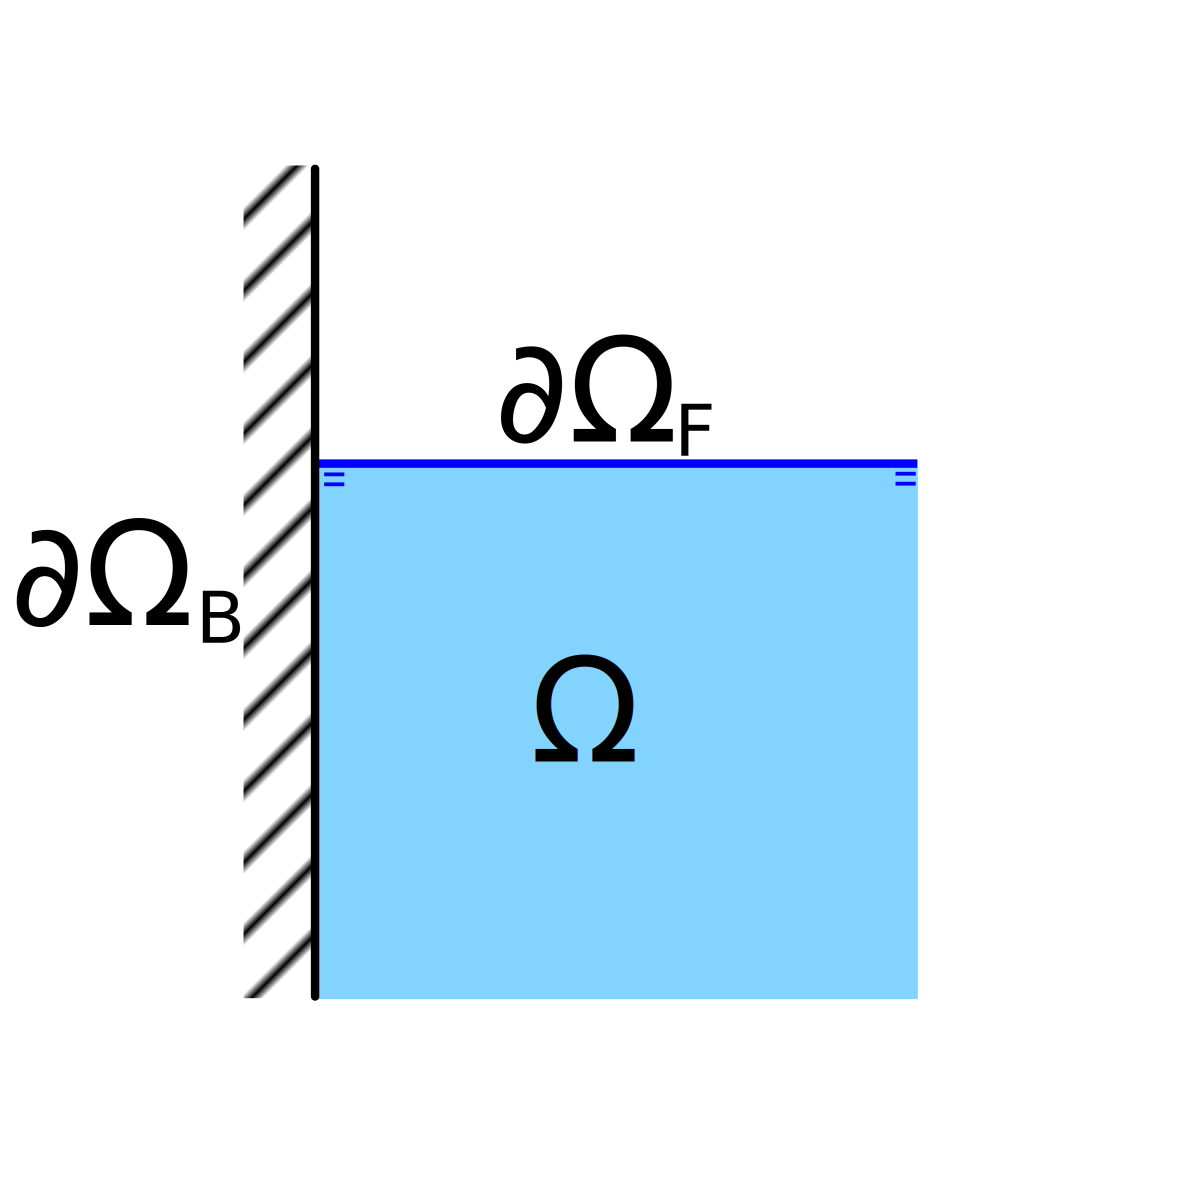
\includegraphics[width=0.4\textwidth]{BC}
  \caption{Boundary conditions scheme}
  \label{fig:aquagpusph:BC}
\end{figure}
%
\subsection{Initial conditions}
%
Since the governing equations \ref{eq:navierstokes} corresponds to an hyperbolic problem,
that must be solved as an initial value problem, the pressure, density and velocity fields
(right hand sides of the equations involved fields) must be known at a initial time $t_0$
where a forward time integration will be performed. In this type of problems backward
time integration is not generally possible.\rc
%
The fields in the initial condition must accomplish the governing equations
\ref{eq:navierstokes}. If the fluid is in rest continuity equation is implicitly
accomplished due to the velocity is null, but fields must be selected in order to get null
accelerations from momentum equation.
%
\section{SPH approximation}
\label{ss:sph_description}
%
\subsection{General}
%
SPH (Smoothed Particle Hydrodynamics) is a numerical method of simulation created at 1977
independently by Lucy (1977) and Gingold \& Monaghan (1977). In this method the fluid is
divided into a set of particles for which the fluid equations are written in a Lagrangian
form, avoiding mesh requirement. Meshfree character of the method is the most attractive
feature because it can be applied to really complex geometries where a mesh generation is not
a good option.\rc
%
SPH was presented as an application of the Monte Carlo method for the resolution of problems
of gas dynamics on astrophysics, but was extended to incompressible flows by Monaghan (1994).
%
\subsection{Continuous model}
\label{ss:sph_continuous}
%
In SPH a kernel $W_h(\bs x)$ is defined as an even function such that
%
\begin{eqnarray}
\int_{-\infty}^{\infty} W_h(\bs y) d\bs y = 1
\end{eqnarray}
%
For practical purposes, the defined kernel $W_h(\bs x)$ vanishes for $\left\vert \bs x \right\vert > sh$,
where $s$ is an integer greater than 0. In \NAME
the \citet{wendland_1995} purposed kernel is mainly used, but other ones are supported and can be selected
with minor changes in the OpenCL code. In table \ref{tables:abstract:kernels} a list with the provided
kernels can be found, but the user can incorporate easily other kernels.\rc
%
The SPH approximation with respect to the kernel $W_h(\bs x)$ of a scalar or vector function $f(\bs x)$
is defined as
%
\begin{eqnarray}
\langle f \rangle (\bs{x}) := \frac{1}{\gamma_h(\bs{x})} \SPHint f(\bs{y}) W_h(\bs{x}-\bs{y}) d\bs{y}
\end{eqnarray}
%
where $\gamma_h(\bs x)$ is the Shepard normalization factor, defined as
%
\begin{eqnarray}
\gamma_h(\bs x) := \SPHint W_h(\bs x - \bs y) d\bs y
\end{eqnarray}
%
with $\Omega$ as the ball of radius $sh$ centred on $\bs x$, subtracting eventually the domain out
of fluid. In the standard SPH formulation Shepard normalization factor is neglected, considering
it $\gamma_h(\bs x) = 1$, that is a good approach far enough of the solid boundary, or near too
if fluid extension based boundary conditions are imposed. Shepard correction can produce some
instabilities, but improves the consistency and is mandatory for De Leffe's type boundary condition
\citep{deleffe_etal_spheric09,ferrand_etal_2012}, that will be discussed later. On the other hand
droping if from the formulation makes it intrinsically conservative \citep{mon2005}, that could be
a really desirable property.\rc
%
The gradient and the divergence of functions can be also interpolated
%
\begin{eqnarray}
\langle \gradient p \rangle (\bs x) = \frac{1}{\gamma_h(\bs x)} \SPHint \gradient p(\bs y) W_h(\bs x - \bs y) d\bs y
\end{eqnarray}
\begin{eqnarray}
\langle \divergence(\bs{u}) \rangle (\bs x) = \frac{1}{\gamma_h(\bs x)} \SPHint \divergence(\bs{u}(\bs y)) W_h(\bs x - \bs y) d\bs y
\end{eqnarray}
%
In these formulas $\gradient p$ and $\divergence(\bs{u})$ are not known. Integrating by parts the
differential operators can be conveniently moved to the kernel function. We will work only over the gradient
operator to show the procedure but analogous treatment is applied to the divergence one.
%
\begin{eqnarray}
\langle \gradient p \rangle (\bs x) = \frac{1}{\gamma_h(\bs x)} \left(
	  \SPHint \gradient \left( p(\bs y) W_h(\bs x - \bs y) \right) d\bs y
	- \SPHint p(\bs y) \gradient W_h(\bs x - \bs y) d\bs y
\right)
\end{eqnarray}
%
If $W_h(\bs x)$ is an even function, $\gradient W_h(\bs x)$ is an antisymmetric one, so we can use
this property to switch the integral terms signs. Also we can use the divergence theorem over the first
integral term.
%
\begin{eqnarray}
\langle \gradient p \rangle (\bs x) = \frac{1}{\gamma_h(\bs x)} \left(
	  \SPHint p(\bs y) \gradient W_h(\bs y - \bs x) d\bs y
	- \SPHboundint p(\bs y) W_h(\bs y - \bs x) \bs n(\bs y) dS(\bs y)
\right)
\end{eqnarray}
%
Where $\partial \Omega$ denotes the boundary of $\Omega$. The contour term has been traditionally neglected
in the literature because authors assume that $p = 0 \in \partial \Omega$\footnote{The almost used boundary
conditions along the solid walls in SPH have consists in fluid extensions, so the contour $\partial \Omega$
has been rely only for the free surface}. In \NAME this boundary integral and the Shepard correction term
can be retained.\rc
%
Regarding Laplacian operator, The 2 most popular formulations to approximate it are
\citet{Monaghan+Gingold:83} form and \citet{Morris+etal:1997} form. \citet{Colagrossi2009} demonstrated that
only the first one provides right dissipation in the presence of a free surface when boundary terms are
discretized, so in \NAME the second way has not been implemented.\rc
%
Assuming that the viscosity coefficients are constant all over the fluid domain, the continuous
formulation of the Monaghan viscous term is:
%
\begin{eqnarray}
\langle \laplacian \bs u \rangle (\bs x) = 
\frac{\mu \, K}{\gamma_a(\bs x) \, \rho(\bs x)} \SPHint
	\frac{
		\left(\bs{u}(\bs y) - \bs{u}(\bs x) \right) \cdot (\bs{y} - \bs{x})
	}{
		\left\vert \bs{y} - \bs{x} \right\vert^2
	} \, \gradient  W_h(\bs y - \bs x) \, d\bs{y}
\end{eqnarray}
%
where $K$ is a parameter depending on the spatial dimension ($K\,=\,6,8,15$, respectively in $1D$,
$2D$ and $3D$).\rc
%
This viscous term is valid far enough of the boundary, and provides right dissipation near the free surface.
Boundary viscous term is added as described by \citet{Maciaetal_PTP_2012} in order to can impose no-slip
boundary conditions in the boundaries.
%
\begin{eqnarray}
\begin{array}{lcl}
\langle \laplacian \bs u \rangle (\bs x) & = &
\dsty{\frac{\mu}{\gamma_a(\bs x) \, \rho(\bs x)}} \left(
	\SPHint K \frac{
		\left(\bs{u}(\bs y) - \bs{u}(\bs x) \right) \cdot (\bs{y} - \bs{x})
	}{
		\left\vert \bs{y} - \bs{x} \right\vert^2
	} \, \gradient  W_h(\bs y - \bs x) \, d\bs{y} \right.
	\vspace{0.3cm} \\ & & 	
    \left. - \dsty{\SPHboundint \left(\bs{u}(\bs y) - \bs{u}(\bs x) \right) \frac{
		 (\bs{y} - \bs{x}) \cdot \bs{n}(\bs{y})
	}{
		\left\vert \bs{y} - \bs{x} \right\vert^2
	} \, W_h(\bs y - \bs x) \, dS(\bs{y})}
    \right)
\end{array}
\end{eqnarray}
%
All this smoothing procedures introduces errors in the representation of functions and operators. These errors
goes to zero as $h \rightarrow 0$, but the convergence order may be different
\citep{MaciaetalPTP,Maciaetal_PTP_2012}.
%
\begin{table}[h!b!p!]\small
	\centering
	\begin{tabular}{| c | c | c | l | }
		\hline
		\cellcolor[rgb]{0.7,0.7,0.7}Kernel & \cellcolor[rgb]{0.7,0.7,0.7}Support \\
		\hline
		Wendland     & $2h$ \\
		\hline
		Cubic spline & $2h$ \\
		\hline
		Gaussian     & $3h$ \\
		\hline
	\end{tabular}
	\caption{\NAME provided kernels.}
	\label{tables:abstract:kernels}
\end{table}
%
\subsection{Discretized model}
\label{ss:sph_discretized}
%
For practical purposes the integrals present on continuous SPH interpolation are solved numerically,
so another error must be considered due to the discretization \citep{Quinlan_06,Amicarelli2011279}.
In order to do it, the space will be discretized placing a set of particles that is treated in a
Lagrangian point of view. $d\bs{y}$ must be then discretized as the volume of the particles, that can
be rewritten such that
%
\begin{eqnarray}
d\bs{y} \approx \frac{m_b}{\rho_b}
\end{eqnarray}
%
allowing us to discretize the operators.
%
\begin{eqnarray}
\label{eq:sph:gradient}
\langle \gradient p \rangle_a = \frac{1}{\gamma_a} \left(
	  \sum\limits_{b \in \mathrm{Fluid}} \frac{p_b}{\rho_b} \gradient W_{ab} m_b
	- \sum\limits_{b \in \mathrm{Boundary}} p_b W_{ab} \bs{n}_b S_b
\right)
\end{eqnarray}
%
In the equation \ref{eq:sph:gradient} the discretized version of the SPH gradient operator over the pressure
field is shown, where the value is computed interpolating it from the neighbour particles and, eventually,
from the neighbour wall elements.\rc
%
In the figure \ref{fig:sph:interpolationscheme} a scheme about the interpolation over a particle labelled
``$a$'' is shown, the index $b$ of the first sum moves along all the fluid particles, but since the kernel
nullifies at a distance $s \, h$, only the particles near enough will be considered.\rc
%
In the figure \ref{fig:sph:wendland} 2D Wendland kernel value is shown. Both kernel value $W$ and
gradient value $\gradient W$ nullifies for distances $\vert \bs{x} \vert > 2 \, h$. Must be noticed that
$\gradient W$ nullifies also for $\vert \bs{x} \vert = 0 \, \mbox{m}$, but not the kernel value.\rc
%
As introduced previously, the weight function $W$ is even, but the gradient $\gradient W$ is an odd
function.\rc
%
In the same way Laplacian operator can be also discretized:
%
\begin{eqnarray}
\begin{array}{lcl}
\langle \laplacian \bs u \rangle_a & = & 
\dsty{\frac{\mu}{\rho_a \, \gamma_a}} \left(\dsty{
    \sum\limits_{b \in \mathrm{Fluid}}
	K \frac{
		\left(\bs{u}_b - \bs{u}_a \right) \cdot (\bs{x}_b - \bs{x}_a)
	}{
		 \rho_b \, \left\vert \bs{x}_b - \bs{x}_a \right\vert^2
	} \, \gradient  W_{ab} \, m_b }\right.
    \vspace{0.3cm} \\ & & \left.\dsty{
    \sum\limits_{b \in \mathrm{Boundary}}
	\left(\bs{u}_b - \bs{u}_a \right)
	\frac{
		 (\bs{x}_b - \bs{x}_a) \cdot \bs{n}_b
	}{
		 \left\vert \bs{x}_b - \bs{x}_a \right\vert^2
	} \, W_{ab} \, S_b}\right)
\end{array}
\end{eqnarray}
%
Since the divergence operator is so quite similar to the gradient, is not introduced here due to will
be discussed a little bit more in the following section.\rc
%
So in the SPH discretized model 2 main spatial variables must be selected:
%
\begin{enumerate}
	\item Kernel height $h$: Set the ball where values will be taken in order to perform the smoothed
	interpolation. as this value goes to zero, the weight function converges to the Dirac's delta one,
	so converges to the real solution as well.
	\item Distance between particles $r$: Set the resolution of the numerical integrals approximation,
	so in the limit of $r \rightarrow 0 \, \mbox{m}$, the integrals are exactly computed.
\end{enumerate}
%
Since $r$ must be lower than interaction distance $s \, h$, usually this 2 key values are changed by $h$
and $h / r$ (formerly $h_{fact}$), or by $r$ and $h / r$\footnote{In \NAME this second approach is applied}.
The kernel height defines the problem resolution therefore, and decreasing this value the number of particles
increase improving the result resolution as values smoothed interpolation (considering that $h_{fact}$ is
preserved constant). The distance between particles, expressed as the ratio $h / r$, defines the number
of neighbours that will interact with each particle, so increasing this value the number of interactions
will increase, and the integrals approximation will be improved.
%
\begin{eqnarray}
\lim_{h \to 0; \, \frac{h}{r} \to \infty} \langle p \rangle = p
\end{eqnarray}
%
The problem complexity is $\mathrm{f} \left((1/h)^3 \,\cdot\, (h/r)^3\right)$ for a $3D$ simulation (time
integration associated complexity is not considered yet) therefore.
%
\begin{figure}[!ht]
  \centering
  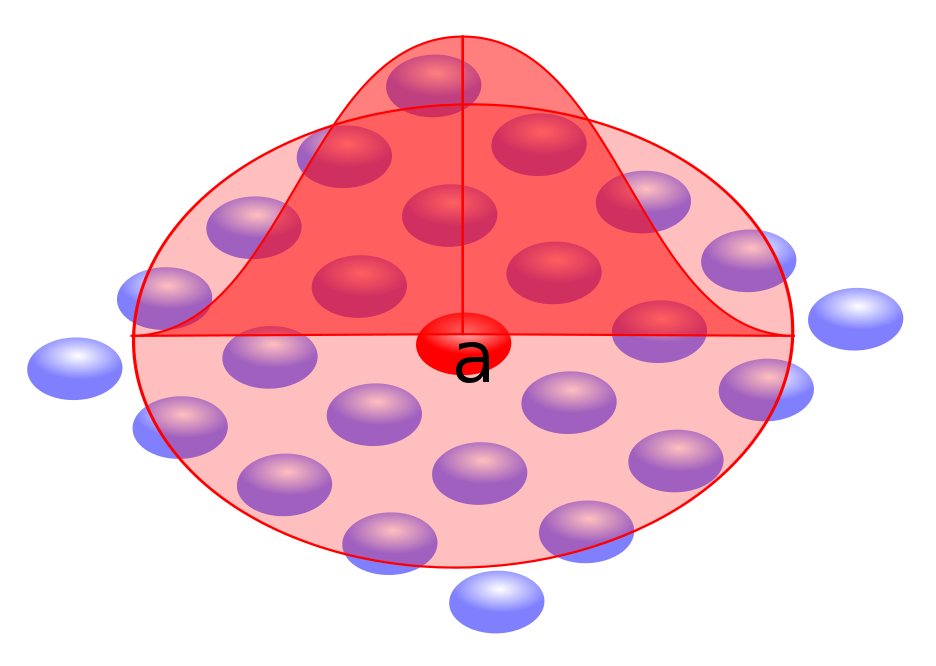
\includegraphics[width=0.5\textwidth]{SPHInterpolation}
  \caption{Discrete SPH interpolation scheme}
  \label{fig:sph:interpolationscheme}
\end{figure}
%
\begin{figure}[!ht]
  \centering
  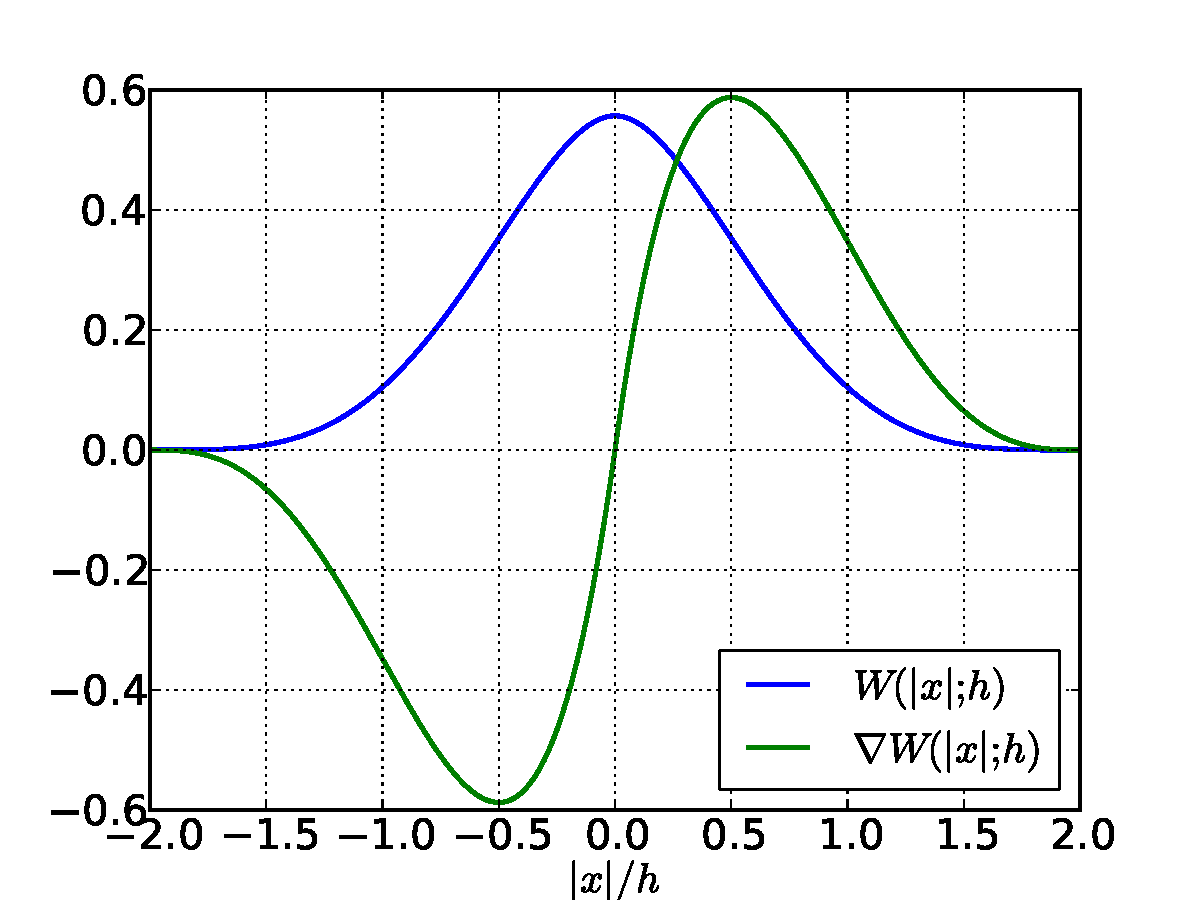
\includegraphics[width=0.8\textwidth]{wendland/wendland2D}
  \caption{2D Wendland Kernel value (and gradient), $h=1 \mbox{m}$}
  \label{fig:sph:wendland}
\end{figure}
%
\subsection{\NAME discretized operators used}
\label{ss:intro:aquagpusph:operators}
%
For conservation considerations, that you can find on \citep{mon2005} and
\citep{Colagrossi2009}, the operators used in \NAME are not the shown on previous
section, but are conveniently modified (formerly simmetrized) as
%
\begin{eqnarray}
\label{eq:aquagpusph:operators}
\begin{array}{lcl}
\dsty{\left\langle \frac{\gradient p}{\rho} \right\rangle_a} & = & 
\dsty{\frac{1}{\gamma_a}} \left(\dsty{
	\sum\limits_{b \in \mathrm{Fluid}}
		\left(\frac{p_a}{\rho_a^2} + \frac{p_b}{\rho_b^2}\right)
	\gradient W_{ab} m_b}\right.
	\vspace{0.1cm} \\ & & \left.\dsty{
	- \sum\limits_{b \in \mathrm{Boundary}}
		\rho_b \left(\frac{p_a}{\rho_a^2} + \frac{p_b}{\rho_b^2}\right)
	 W_{ab} \, \bs{n}_b \, S_b}\right)
\vspace{0.3cm} \\

\dsty{\left\langle \rho \, \divergence(\bs{u}) \right\rangle_a} & = & 
\dsty{\frac{1}{\gamma_a}} \left(\dsty{
	\sum\limits_{b \in \mathrm{Fluid}}
		\left(\bs{u}_b - \bs{u}_a\right)
	\gradient W_{ab} m_b}\right.
	\vspace{0.1cm} \\ & & \left.\dsty{
	- \sum\limits_{b \in \mathrm{Boundary}}
		\rho_b \left(\bs{u}_b - \bs{u}_a\right) \cdot n_b
	 W_{ab} \, S_b}\right)
\vspace{0.3cm} \\

\langle \laplacian \bs u \rangle_a & = & 
\dsty{\frac{\mu}{\rho_a \, \gamma_a}} \left(\dsty{
    \sum\limits_{b \in \mathrm{Fluid}}
	K \frac{
		\left(\bs{u}_b - \bs{u}_a \right) \cdot (\bs{x}_b - \bs{x}_a)
	}{
		 \rho_b \, \left\vert \bs{x}_b - \bs{x}_a \right\vert^2
	} \, \gradient  W_{ab} \, m_b }\right.
    \vspace{0.1cm} \\ & & \left.\dsty{
    \sum\limits_{b \in \mathrm{Boundary}}
	\left(\bs{u}_b - \bs{u}_a \right)
	\frac{
		 (\bs{x}_b - \bs{x}_a) \cdot \bs{n}_b
	}{
		 \left\vert \bs{x}_b - \bs{x}_a \right\vert^2
	} \, W_{ab} \, S_b}\right)
\end{array}
\end{eqnarray}
%
The operators shown above results from the divergence theorem application over the
operators to interpolate, and have the main advantage that are ever convergent for
constant fields (of pressure and velocity).\rc
%
Weakly compressible SPH formulation carry some high frequency pressure oscillations
caused by the small density fluctuations with the huge incompressibility requirements.
In order to solve partially this effect the density field, that results from a
evolution process, can be reinitialized from particles positions using the property
%
\begin{eqnarray}
\dsty{\left\langle \rho \right\rangle_a} =  
\dsty{\frac{1}{\gamma_a}} \dsty{ \sum\limits_{b \in \mathrm{Fluid}} W_{ab} m_b}
\end{eqnarray}
%
That allows to recover a smooth density field. This correction is not usually
recommended due to can carry some instabilities, but when applied, in almost cases
this correction is only used letting some time steps between corrections. In \NAME
you can select how many steps must run before apply this correction, or simply don't
apply it.
%
\subsection{Boundary conditions}
%
\subsubsection{Free surface boundary conditions}
%
Free surface kinematic and dynamic boundary conditions are automatically accomplished
in the W-SPH formulation, so only the consistency of the operators must be guaranteed.
%
Considering null the ambient pressure $p_0$ in the state equation of the governing
ones \ref{eq:navierstokes} no pressure extra condition has to be imposed at the free
surface as \citet{Colagrossi2009} demonstrates.\rc
%
Unfortunately near the free surface gradient, divergence an Laplacian operators shown in the
equations \ref{eq:aquagpusph:operators} are convergent, but not consistent due to the
result converges to a wrong value. The half good news is that, since the results converges,
and the region where the results are inconsistent is confined to a distance $s \, h$ of
the free surface, in a integral point of view the operators introduced converges to the
right solution with order $\mathcal{O}(h)$.\rc
%
In order to get consistent gradient, divergence an Laplacian operators near the free surface,
as the most desirable ones, track process over the free surface is needed, with a significant
regression in the computational efficiency and robustness.\rc
%
So, assuming an inconsistency near the free surface that is bounded, with an ambient pressure
such that $p_0 = 0 \, \mbox{Pa}$, no additional conditions needs to be imposed in the free
surface therefore.\rc
%
All these assumptions are refereed to monophasic simulations, that are the mainly used in \NAME
simulations.
%
\subsubsection{Solid boundary conditions}
\label{ss:sph:discrete:BC}
%
Regarding solid body boundary conditions \NAME allows to use most popular SPH to modeling techniques:
%
\begin{enumerate}
	\item \textbf{Fixed particles}: Also known as dummy particles, this method consists
	of extending the fluid domain across the wall with fluid particles, fixing their motion.
	This is the boundary condition traditionally used on SPH method.
	\item \textbf{Ghost particles}: This method consist on extending the fluid domain across
	the wall as well, but in this case the fluid at the other side is obtained as mirroring
	process over the fluid domain. It has been developed as an improvement of the previous one.
	\item \textbf{Elastic bounce}: In this method the particles near to the wall, that will
	trespass it, are treated with an elastic bounce model, where an elastic bounce factor is
	used to set the amount of energy conserved in the interaction. This boundary condition
	is not designed to use it alone, but can be mixed with the other ones in order to can
	manage the particles that will cross over the walls without crashing the simulation.
	\item \textbf{Boundary integrals}: Introduced by \citet{deleffe_etal_spheric09},
	and formalized by \citet{ferrand_etal_2012}, in this method the boundary integrals
	are numerically solved along the walls. Is the most recent one, but the consistency
	has been probed by \citet{Maciaetal_PTP_2012}, with the examples performed with \NAME
	software.
\end{enumerate}
%
Each boundary condition type has some advantages, and some combinations of them can be applied in
your simulations. Boundary conditions introduced are described and discussed in detail at section
\ref{ss:aquagpusph:boundaries}, where their algorithmic details are discussed.
%
\subsection{Initial condition}
\label{ss:sph:discrete:initialconditions}
%
As introduced in section \ref{ss:sph_discretized}, you must provided a set of particles in the
initial time instant $t_0$. The initial condition must accomplish the governing equations
\ref{eq:navierstokes}. The most frequently used initial condition is a fluid in rest, so we are
focused in this particular case, describing the process to generate the particles.\rc
%
Since the fluid is in rest, and velocity is null therefore, so the continuity equation is implicitly
accomplished. Regarding the momentum equation, if a volumetric force exist (for instance the gravity
force), a pressure gradient must be forced in order to get null accelerations (formerly known as the
hydrostatic pressure), such that
%
\begin{eqnarray}
p = p_0 + \rho_0 \, \bs{g} \cdot \bs{z}
\end{eqnarray}
%
Where $p_0 = 0 \, \mbox{Pa}$, and $z = 0 \, \mbox{m}$ in the free surface. But the state equation impose
a relation between the density field and the pressure field, so the density field provided by the
user must be set as follows (pressure field is not an input variable but is computed using the EOS
\ref{eq:governing_eqns:field_eqns:eos:arfm_2012} when needed):
%
\begin{eqnarray}
\rho = \rho_0 \left( \frac{\gamma \, \bs{g} \cdot \bs{z}}{c_s^2} + 1 \right)^{\frac{1}{\gamma}}
\end{eqnarray}
%
SPH method, as described in section \ref{ss:sph_continuous}, is based on the hypothesis that the
differential of volume $d\bs{y}$ is constant, so the particles volume must be constant as well.
In order to preserve this main condition the particles mass must be computed as follow:
%
\begin{eqnarray}
m = \frac{\mathcal{V}}{\rho}
\end{eqnarray}
%
Where $\mathcal{V}$ is the volume associated to each particle, that in the case of a 3D Cartesian
particles distribution with a distance between particles $\bs r$, allows us to write that
%
\begin{eqnarray}
\mathcal{V} = \bs{r}^3
m = \frac{\bs{r}^3}{\rho}
\end{eqnarray}
%
\subsection{Time numerical integration}
\label{ss:sph:discrete:timestep}
%
In order to approximate numerically the solution of the problem the time integration is discretized
as well.\rc
%
One of the key features of the W-SPH model is that is a purely explicit formulation, so a variable
can be defined in a time instant $t_{n+1}$ as function of known data in a time instant $t_n$, i.e.:
%
\begin{eqnarray}
X \bigg\vert_{\dsty{t_{n+1}}} = \mathrm{F}\left(
	X \bigg\vert_{\dsty{t_{n}}},
	\frac{d X}{dt} \bigg\vert_{\dsty{t_{n}}},
	\frac{d^2 X}{dt^2} \bigg\vert_{\dsty{t_{n}}},
	\cdots; \Delta t
	\right)
\end{eqnarray}
%
The function $\mathrm{F}$ is known as the scheme. Better schemes increase the convergence rate, so
allows to increase the time step in order to get similar errors\footnote{One of the critical points
in the SPH performance is the small time steps involved}, however almost high order time integrating
schemes requires several derivatives computation, that is too computational expensive in SPH. In
AQUAgpusph a quasi-second order method, that only requires one derivative computation per time step,
Leap-Frog method is used \citep{souto2006}, with the main advantage that only one time derivative
is needed by each time step.
%
%
\begin{enumerate}
	\item Predictor:
	\begin{eqnarray}
	\label{eq:sph:discrete:timestep:predictor}
	\begin{array}{lcl}
	\dsty{\dot{\bs{x}}_{t+dt}^{\mathrm{pred}}} & = & 
	\dot{\bs{x}}_{t} + 
	dt \left(
		\ddot{\bs{x}}_{t} + g
	\right)
	\vspace{0.3cm} \\
	\dsty{\bs{x}_{t+dt}^{\mathrm{pred}}} & = &
	\bs{x}_{t} + 
	dt \, \dot{\bs{x}}_{t} + 
	\dsty{\frac{dt^2}{2}} \left(
		\ddot{\bs{x}}_{t} + g
	\right)
	\vspace{0.3cm} \\
	\dsty{\rho_{t+dt}^{\mathrm{pred}}} & = & 
	\rho_{t} + 
	dt \, \dot\rho_{t}
	\end{array}
	\end{eqnarray}

	\item SPH interactions:
	\begin{eqnarray}
	\label{eq:sph:discrete:timestep:interactions}
	\begin{array}{lcl}
	\ddot{\bs{x}}_{t+dt} & \leftarrow & \mbox{SPH}
	\\
	\dot\rho_{t+dt} & \leftarrow & \mbox{SPH}
	\end{array}
	\end{eqnarray}

	\item Corrector:
	\begin{eqnarray}
	\label{eq:sph:discrete:timestep:corrector}
	\begin{array}{lcl}
	\dsty{\dot{\bs{x}}_{t+dt}} = 
	\dsty{\dot{\bs{x}}_{t+dt}^{\mathrm{pred}}} + 
	\dsty{\frac{dt^2}{2}} \left(
		\ddot{\bs{x}}_{t+dt} - \ddot{\bs{x}}_{t}
	\right)
	\vspace{0.3cm} \\
	\dsty{\bs{x}_{t+dt}} = \dsty{\bs{x}_{t+dt}^{\mathrm{pred}}}
	\vspace{0.3cm} \\
	\dsty{\rho_{t+dt}} = 
	\dsty{\rho_{t+dt}^{\mathrm{pred}}} + 
	\dsty{\frac{dt}{2}} \left(
		\dot\rho_{t+dt} - \dot\rho_{t}
	\right)
	\end{array}
	\end{eqnarray}
\end{enumerate}
%
In order to get a stable time integration time step must be selected such that
%
\begin{eqnarray}
\label{eq:sph:discrete:timestep:dtmax}
dt \le \frac{h}{\max(10 \, \vert \bs{u} \vert, \, c_s)}
\end{eqnarray}
%
In the section \ref{ss:sph_discretized} the complexity of one time step has been introduced, but of
course this complexity increases linearly with the time steps required, so 3 algorithmic complexities
must be considered:
%
\begin{enumerate}
	\item Number of particles $N$: The number of particles is conditioned by the kernel height $h$,
	and defines the spatial resolution implying a complexity of $\mathcal{O}(3)$.
	\item Number of neighbours $M$: The number of neighbours is conditioned by the ratio $h / r$, and
	defines the quality of the numerical integrals approximation implying a complexity of
	$\mathcal{O}(3)$.
	\item Number of time steps: The number of time steps is conditioned by the time step $dt$, that
	depends directly on kernel height $h$, implying a complexity of $\mathcal{O}(1)$.
\end{enumerate}
%
So, if we increase the number of particles but not the number of neighbours, time step will be reduced
and then complexity goes as $N^4$.\rc
%
At the other hand, if the number of particles is constant but the number of neighbours is increased,
kernel height increases therefore resulting in higher time steps, so the complexity goes as $M^2$.\rc
%
So the method complexity goes as $N^4 \, M^2$, that shows that you must be careful with the convergence
because time consumed by the simulations will grows too fast ($\mathcal{O}(6)$ in the worst case).
%
\chapter{Install \NAME}
\label{s:install}
%
\section{General}
%
\NAME can be downloaded from
%
\begin{center}
\url{http://canal.etsin.upm.es/aquagpusph/descargas.php}
\end{center}
%
The process to configure, build and install is described below. The files
uploaded to this web page are the latest stable version, but optionally
you can download the developers version, that has more fresh features, but
can carry some bugs and unstabilities. Developers version is allocated in
\href{https://github.com/}{github}, so you must have git installed on your
system to access to the source code. To download the developers package
version execute
%
\begin{verbatim}
git clone git://github.com/jlcercos/aquagpusph.git
\end{verbatim}
%
that will generate a folder called ``aquagpusph'' with the package inside.\rc
%
The instructions included below are valid for both the stable and the
developers versions, but some additional dependencies and configuration can
be missed.\rc
%
For the moment no specific GNU/Linux distributions installable packages have
been created.
%
\section{Dependencies}
%
\NAME has some dependencies that must be installed before. Almost dependencies
are mandatory, but exist other dependencies that can be optionally ignored
depending on the needed capabilities on \NAME built program.\rc
%
Dependencies are classified in 4 categories therefore:
%
\begin{enumerate}
	\item Mandatory: \NAME needs the dependency available on system in order to
	run.
	\item Optional: If dependency is not available, \NAME can be built, but some
	features will be disabled.
	\item Recommended: If dependency is not available, \NAME can be built with
	all the features, but some
	additional package characteristics may not run.
	\item Suggested: \NAME can have some synergies with other softwares, for
	preporcessing or postprocessing for instance.
\end{enumerate}
%
In table \ref{tables:install:dependencies} you can see the list of dependencies
required. Each dependency can require more other dependencies that will not be
documented. Take into account the following considerations:
%
\begin{enumerate}
	\item OpenCL is a little bit special dependency due to is really hardware
	depending, therefore at the web page only OpenCL specification will found.
	We encourage you to contact your hardware provider in order to know the
	best way to install it.
	\item NCurses can be used to perform smart screen output, that can revert
	on slightly reduced computational time. Any relevant functionality will
	be lost if \NAME is compiled without NCurses support therefore.
	\item While H5Part was the main \NAME output format in previous versions, 
	it has been replaced by VTK files (H5Part has been declared as an outdated 
	format).
	\item Doxygen and Graphviz are only needed if you want to build Doxygen
	developers documentation. This documentation is mainly oriented to 
	developers, but can be really useful for users in some number of cases, so 
	is strongly recommended to build it.
\end{enumerate}
%
\begin{table}[h!b!p!]\small
	\centering
	\begin{tabular}{| c | c | c | }
		\hline
		\cellcolor[rgb]{0.7,0.7,0.7}Dependency &\cellcolor[rgb]{0.7,0.7,0.7}Status &\cellcolor[rgb]{0.7,0.7,0.7}Web page\\
		\hline
		CMake    & Mandatory   & \url{http://www.cmake.org} \\
		\hline
		xerces-c & Mandatory   & \url{http://xerces.apache.org/xerces-c} \\
		\hline
		Python   & Mandatory   & \url{http://www.python.org} \\
		\hline
		OpenCL   & Mandatory   & \url{http://www.khronos.org/opencl} \\
		\hline
		Eigen3   & Mandatory   & \url{http://eigen.tuxfamily.org/index.php} \\
		\hline
		libmatheval & Mandatory   & 
		\url{https://www.gnu.org/software/libmatheval} \\
		\hline
		Ncurses  & Optional    & \url{http://www.gnu.org/software/ncurses/ncurses.html} \\
		\hline
		VTK      & Optional    & \url{http://www.vtk.org} \\
		\hline
		Doxygen  & Recommended & \url{http://www.doxygen.org} \\
		\hline
		Graphviz & Recommended & \url{http://www.graphviz.org} \\
		\hline
		matplotlib & Suggested   & \url{http://matplotlib.org} \\
		\hline
		numpy & Suggested   & \url{http://www.numpy.org} \\
		\hline
		PyQt4 & Suggested   & 
		\url{http://www.riverbankcomputing.com/software/pyqt/intro} \\
		\hline
		gnuplot  & Suggested   & \url{http://www.gnuplot.info} \\
		\hline
		ParaView & Suggested   & \url{http://www.paraview.org/} \\
		\hline
	\end{tabular}
	\caption{\NAME dependencies.}
	\label{tables:install:dependencies}
\end{table}
%
\section{Install}
%
\subsection{General}
%
\NAME use \href{http://www.cmake.org}{CMake} to the configure, build and 
install process. CMake installation process is performed in 3 steps therefore:
%
\begin{enumerate}
	\item \textbf{CMake configuration}: In this stage main options and features
	that the built version of \NAME will have.
	\item \textbf{Compilation}: In this step the source code is compiled into a
	binary ready to be launched.
	\item \textbf{Install}: This step is optional, aiming to install the 
	software on the system in order to be available for all the users of the 
	computer.
\end{enumerate}
%
To perform the CMake configuration process 2 ways are described.
%
\subsection{CMake configuration}
\label{sss:install:cmake}
%
To start configuring CMake you can run the following command on the folder 
where you downloaded \NAME sources:
%
\begin{verbatim}
cmake .
\end{verbatim}
%
That will configure \NAME with default options. You can modify some options, 
for instance, to change installation prefix from $\mbox{/usr/local}$ to 
$\mbox{/usr}$ folder, and build Release version, you can launch following 
command:
%
\begin{verbatim}
cmake -D CMAKE_INSTALL_PREFIX:PATH=/usr -D CMAKE_BUILD_TYPE:STRING=Release .
\end{verbatim}
%
In \url{http://www.cmake.org/Wiki/CMake_Useful_Variables} web page you can 
find a list with the most commonly CMake used options. Also \NAME provides 
some additional options:
%
\begin{enumerate}
	\item \textbf{AQUAGPUSPH\_3D}: ON to build 3D \NAME version, OFF to build 
	2D version. \NAME 2D and 3D versions can be installed on the same system. 
	Be mindful that 3D version must not be used to perform 2D simulations.
	\item \textbf{AQUAGPUSPH\_BUILD\_DOC}: ON to build 
	\href{http://www.doxygen.org}{Doxygen} developers documentation, OFF 
	otherwise. Requires \href{http://www.doxygen.org}{Doxygen} and 
	\href{www.graphviz.org}{Graphviz} packages installed in the system.
	\item \textbf{AQUAGPUSPH\_BUILD\_EXAMPLES}: ON to generate the examples. 
	Generated examples are the associated to the selected 2D/3D version.
	\item \textbf{AQUAGPUSPH\_USE\_NCURSES}: ON to build \NAME with NCurses 
	output terminal, OFF otherwise. NCurses has more efficient screen streamed 
	functionality, so you can win some performance using it.
	\item \textbf{AQUAGPUSPH\_USE\_VTK}: ON to build \NAME with VTK output 
	support, OFF otherwise. In \NAME- \VERSION VTK is the only valid output 
	format for the particles files, so it is mandatory to can process 
	visualizations of the simulations.
\end{enumerate}
%
\subsection{CMake configuration with ccmake}
%
I order to simplify the process you can use ccmake\footnote{Or eventually 
CMake-GUI} to configure \NAME with a more friendly user interface (Of course 
you must install ccmake before). Simply launch the command:
%
\begin{verbatim}
ccmake .
\end{verbatim}
%
If you did not configure \NAME before, an empty cache page will shown up, press
\textbf{'c'} key to perform initial default configuration. After some seconds 
working, errors, warnings, and most relevant selected options report will be 
returned; press \textbf{'e'} key to continue.\rc
%
Now some options are shown in order to allow you to edit them.
%
Probably you want to edit CMAKE\_INSTALL\_PREFIX too. Take care about
CMAKE\_BUILD\_TYPE, Debug mode is a lot of more resources consuming and slow, 
therefore it's strongly recommended to let Release mode for almost users.\rc
%
After this, press \textbf{'c'} key in order to configure the package again. 
Repeat the process until no new options are shown (that are marked with an 
asterisk), and no more errors are reported.
%
At this point ccmake will offer generating final project pressing \textbf{'g'} 
key.\rc
%
Same options introduced in \ref{sss:install:cmake} can be set using ccmake.
%
\subsection{Compilation}
%
After the configuration process you can start the compilation in order to 
create the binary.
%
You can launch the following command:
%
\begin{verbatim}
make all
\end{verbatim}
%
Since \NAME build process is not really time consuming parallel compiling 
process is not generally needed, but of course you can set several processors 
building simultaneously.
%
For instance, if you want to use 8 cores you can type:
%
\begin{verbatim}
make -j8
\end{verbatim}
%
Additionally, if you want to get more info about the building process, you can 
use VERBOSE flag:
%
\begin{verbatim}
make VERBOSE=1
\end{verbatim}
%
This will report the command executed to compile/generate each file.
%
\subsection{Install}
%
\NAME can be used without installing it, see generated examples to learn more 
about this, but if \NAME must be provided to several users probably you want 
to install it typing:
%
\begin{verbatim}
make install
\end{verbatim}
%
Note that depending the selected installation folder you may need administrative permissions.
%

% -------------------------------
% Case generation explanation
% -------------------------------
\chapter{Case setup options glossary}
\label{s:caseSetup}
%
\section{General}
%
\NAME has a powerful XML files input interface used to setup simulation cases.
Those files can be easily structured as a tree with the including capabilities.
XML is a standard file format where a schematic structure of the files is
allowed. You can learn more about XML syntax and possibilities at next web page:
%
\begin{center}
    \url{http://www.w3.org/XML}
\end{center}
%
The objective of this chapter is to show all the available settings and switches
that can be established for a \NAME simulation, but for a practical approach
to generating and running simulations please refer to chapter \ref{s:examples},
where \NAME package examples are discussed.
%
\section{XML definition}
%
\subsection{General}
%
Each XML file must have the following structure:
%
\begin{verbatim}
<?xml version="1.0" ?>
<sphInput>
    ...
</sphInput>
\end{verbatim}
%
Of course all the XML valid syntax can be used in these files
(i.e.- Comments, ...). In the table \ref{tables:caseSetup:XML:Options} all the
valid options that can be set at sphInput group are described. In the table
\ref{tables:caseSetup:XML:Groups} the valid sections into sphInput group are
described. You can add several several times each section which, depending on
the settings affected, will overwrite or add the information.
%
The different group tags are now discussed.
%
\begin{table}[h!b!p!]\small
	\centering
	\begin{tabular}{| c | c | c | l | }
		\hline
		\cellcolor[rgb]{0.7,0.7,0.7}Tag & \cellcolor[rgb]{0.7,0.7,0.7}Attributes & \cellcolor[rgb]{0.7,0.7,0.7}Valid values & \cellcolor[rgb]{0.7,0.7,0.7}Description \\
		\hline
		Include & file & XML file path & Specified XML file will processed before continuing parsing this file. \\
		        &      &               & You can include as many files as you want. \\
		\hline
	\end{tabular}
	\caption{Valid option tags in the sphInput group.}
	\label{tables:caseSetup:XML:Options}
\end{table}
%
\begin{table}[h!b!p!]\small
	\centering
	\begin{tabular}{| c | c | c | l | }
		\hline
		\cellcolor[rgb]{0.7,0.7,0.7}Tag & \cellcolor[rgb]{0.7,0.7,0.7}Attributes & \cellcolor[rgb]{0.7,0.7,0.7}Valid values & \cellcolor[rgb]{0.7,0.7,0.7}Description \\
		\hline
		Settings       & \textit{none} & \textit{none}       & General \NAME parameters can be set here. \\
		\hline
		OpenCL         & \textit{none} & \textit{none}       & OpenCL kernels to compute can be selected here. \\
		\hline
		Timing         & \textit{none} & \textit{none}       & Simulation time control directives are set here. \\
		\hline
		SPH            & \textit{none} & \textit{none}       & SPH method relevant data must be provided here. \\
		\hline
		Fluid          & n             & Number of particles & Fluid data must be provided in this section. \\
		               &               &                     & Each Fluid section will add new fluid to simulation. \\
		\hline
		Sensors        & \textit{none} & \textit{none}       & Sensor (or probes) can be specified in this section. \\
		\hline
		Movements      & \textit{none} & \textit{none}       & Motions to apply to the boundaries can be set here. \\
		\hline
		GhostParticles & \textit{none} & \textit{none}       & Ghost particles boundary can be set here. \\
		\hline
	\end{tabular}
	\caption{Valid section tags in the sphInput group.}
	\label{tables:caseSetup:XML:Groups}
\end{table}
%
\subsection{Settings group}
\label{sss:XML:Settings}
%
This group is used to set some \NAME general settings, that are not really
related to specific simulation. Table \ref{tables:caseSetup:Settings:Options}
shows all the valid options that can be set in this group.
%
\begin{table}[h!b!p!]\small
	\centering
	\begin{tabular}{| c | c | c | l | }
		\hline
		\cellcolor[rgb]{0.7,0.7,0.7}Tag & \cellcolor[rgb]{0.7,0.7,0.7}Attributes & \cellcolor[rgb]{0.7,0.7,0.7}Valid values & \cellcolor[rgb]{0.7,0.7,0.7}Description \\
		\hline
		Verbose & level & 0 & No verbose. \\
		        &       & 1 & Relevant data will be printed each frame. \\
		        &       & 2 & Relevant data will be printed each time step. \\
		\hline
		Device  & platform & id  & The OpenCL platform to use.\\
                & device   & id  & The device (inside the platform) to use. \\
                & type     & ALL & All the types of variables can be chosen. \\
                &          & CPU & Just CPU devices will be available. \\
                &          & GPU & Just GPU devices will be available. \\
                &          & ACCELERATOR & Just accelerators will be 
                available. \\
                &          & DEFAULT & Just the default OpenCL device will be 
                available. \\
		\hline
	\end{tabular}
	\caption{Valid settings option tags.}
	\label{tables:caseSetup:Settings:Options}
\end{table}
%
\subsection{OpenCL}
\label{sss:XML:OpenCL}
%
This group is used to set the OpenCL kernels that will be used to perform the
simulation. Table \ref{tables:caseSetup:OpenCL:Options} shows all the valid
options that can be set in this section.\rc
%
\NAME provides a version of each OpenCL kernel, but you can create custom
kernels in order to modify the software behaviour conveniently, with the
restriction that new kernels must preserve input parameters (sorted as the
original one).
%
\begin{table}[h!b!p!]\small
	\centering
	\begin{tabular}{| c | c | c | l | }
		\hline
		\cellcolor[rgb]{0.7,0.7,0.7}Tag & \cellcolor[rgb]{0.7,0.7,0.7}Attributes & \cellcolor[rgb]{0.7,0.7,0.7}Valid values & \cellcolor[rgb]{0.7,0.7,0.7}Description \\
		\hline
		Predictor & file & File path & Kernel file used at Leap-frog predictor stage. \\
		          &      &           & File extension (.cl) will appended automatically. \\
		\hline
		LinkList          & file & File path & Kernel file used to perform the Link-List, \\
		                  &      &           & i.e.- In-cell particles localization. \\
		                  &      &           & File extension (.cl) will appended automatically. \\
		\hline
		Rates             & file & File path & Kernel file used to perform particles interaction. \\
		                  &      &           & File extension (.cl) will appended automatically. \\
		\hline
		Corrector         & file & File path & Kernel file used at Leap-frog corrector stage. \\
		                  &      &           & File extension (.cl) will appended automatically. \\
		\hline
		TimeStep          & file & File path & Kernel file used to compute time step. \\
		                  &      &           & File extension (.cl) will appended automatically. \\
		\hline
		Reduction         & file & File path & Kernel file used to perform 
		reductions of variables \\
		                  &      &           & File extension (.cl) will appended automatically. \\
		\hline
		RadixSort         & file & File path & Kernel file used to sort particles by cell location. \\
		                  &      &           & File extension (.cl) will appended automatically. \\
		\hline
		Shepard           & file & File path & Kernel file used to perform 0th order correction. \\
		                  &      &           & File extension (.cl) will appended automatically. \\
		\hline
		Domain            & file & File path & Kernel file used to find and destroy particles out \\
		                  &      &           & of domain. \\
		                  &      &           & File extension (.cl) will appended automatically. \\
		\hline
		ElasticBounce     & file & File path & Kernel file used to perform simple wall boundary \\
		                  &      &           & condition. \\
		                  &      &           & File extension (.cl) will appended automatically. \\
		\hline
		DeLeffe           & file & File path & Kernel file used to perform DeLeffe wall boundary \\
		                  &      &           & condition. \\
		                  &      &           & File extension (.cl) will appended automatically. \\
		\hline
		DensInterpolation & file & File path & Kernel file used to perform density reinitialization. \\
		                  &      &           & File extension (.cl) will appended automatically. \\
		\hline
		Torque            & file & File path & Kernel file used to compute force and torque. \\
		                  &      &           & File extension (.cl) will appended automatically. \\
		\hline
		Bounds            & file & File path & Kernel file used to compute 
		fluid bounds. \\
		                  &      &           & File extension (.cl) will 
		                  appended automatically. \\
		\hline
		Energy            & file & File path & Kernel file used to compute 
		fluid energy. \\
		                  &      &           & File extension (.cl) will 
		                  appended automatically. \\
		\hline
		Portal            & file & File path & Kernel file used to perform particles teleporting. \\
		                  &      &           & File extension (.cl) will appended automatically. \\
		\hline
	\end{tabular}
	\caption{OpenCL kernels tags.}
	\label{tables:caseSetup:OpenCL:Options}
\end{table}
%
\subsection{Timing group}
\label{sss:XML:Timing}
%
This group is used to set simulation time stepping controls. Table
\ref{tables:caseSetup:Timing:Options} shows all the valid options
that can be set in this section.\rc
%
The minimum time step and the Courant factor are not affecting if the time 
step is not selected as ``Variable''.
%
\begin{table}[h!b!p!]\small
	\centering
	\begin{tabular}{| c | c | c | c | c | c | l | }
		\hline
		\cellcolor[rgb]{0.7,0.7,0.7}Tag & \cellcolor[rgb]{0.7,0.7,0.7}Attribute & \cellcolor[rgb]{0.7,0.7,0.7}Values & \cellcolor[rgb]{0.7,0.7,0.7}Attributes & \cellcolor[rgb]{0.7,0.7,0.7}Values & \cellcolor[rgb]{0.7,0.7,0.7}Attributes & \cellcolor[rgb]{0.7,0.7,0.7}Values \\
		\hline
		Option & name & Start &        &         & value  & Starting time. \\
		Option & name & Stop  & type   & Time    & value  & End time. \\
		       &      &                &         & Frames & value & Number of 
		       frames. \\
		       &      &                &        &         &       & (Can be 
		       mixed with time stop \\ 
		       &      &                &        &         &       & criteria) \\ 
		\hline
		       & name & Timestep       & value  & Variable &       & (Time 
		       step recomputed)\\
		       &      &                &        & Fix     & value & (Time step 
		       computed at start) \\
		       &      &                &        & time [s] & & \\
		\hline
		       & name & MinTimeStep    &        &         & value & Minimum 
		       allowed time step\\
		\hline
		       & name & Courant        &        &         & value & Courant 
		       factor\\
		\hline
		       & name & LogFile        & type   & No      &       & \\
		       &      &                &        & FPS     & value & Frames per second. \\
		       &      &                &        & IPF     & value & Iterations per frame. \\
		       &      &                &        &         &       & (Can be 
		       mixed with FPS) \\ 
		\hline
		       & name & EnFile        & type   & No      &       & \\
		       &      &                &        & FPS     & value & Frames per 
		       second. \\
		       &      &                &        & IPF     & value & Iterations 
		       per frame. \\
		       &      &                &        &         &       & (Can be 
		       mixed with FPS) \\ 
		\hline
		       & name & BoundsFile     & type   & No      &       & \\
		       &      &                &        & FPS     & value & Frames per 
		       second. \\
		       &      &                &        & IPF     & value & Iterations 
		       per frame. \\
		       &      &                &        &         &       & (Can be 
		       mixed with FPS) \\ 
		\hline
		       & name & Output         & type   & No      &       & \\
		       &      &                &        & FPS     & value & Frames per second. \\
		       &      &                &        & IPF     & value & Iterations per frame. \\
		       &      &                &        &         &       & (Can be 
		       mixed with FPS) \\ 
		\hline
	\end{tabular}
	\caption{Time control valid tags.}
	\label{tables:caseSetup:Timing:Options}
\end{table}
%
\subsection{SPH}
\label{sss:XML:SPH}
%
This group is used to set SPH method related settings. Table
\ref{tables:caseSetup:SPH:Options} shows all valid options that
can be set in this section.\rc
%
$\gamma$ value is a factor involved in the EOS
\ref{eq:governing_eqns:field_eqns:eos:arfm_2012}.\rc
%
Sound speed must be selected, at least, 10 times greater than the
maximum expected fluid velocity along the simulation. Sound speed
affects directly to the fluid compressibility, so higher sound
speed implies simulation improvements, but is too much computing
expensive (due to a time step reduction).\rc
%
In the equation \ref{eq:sph:discrete:timestep:dtmax} the time step
that must be selected is described (how to setup the time step is
described in the section \ref{sss:XML:Timing}), but in order to
reduce the Courant number you can setup a time step divisor
\textbf{DivDt}.\rc
%
\textbf{LLSteps} steps is the number of time steps between Link-List
computations, so a small performance can be win. For almost cases is
strongly recommended to let \textbf{LLSteps} = 1.\rc
%
The density interpolation (formerly density reinitialization) has been
described in the section \ref{ss:intro:aquagpusph:operators}. With
\textbf{DensSteps} option you may set the number of time steps that
will be computed before each density interpolation.\rc
%
The boundary conditions has been introduced in the section
\ref{ss:sph:discrete:BC}.\rc
%
Finally domain can be used to destroy the particles out of it,
transforming them into 0 mass fixed particles.
%
\begin{table}[h!b!p!]\small
	\centering
	\begin{tabular}{| c | c | c | c | c | }
		\hline
		\cellcolor[rgb]{0.7,0.7,0.7}Tag & \cellcolor[rgb]{0.7,0.7,0.7}Attribute & \cellcolor[rgb]{0.7,0.7,0.7}Values & \cellcolor[rgb]{0.7,0.7,0.7}Attributes & \cellcolor[rgb]{0.7,0.7,0.7}Values \\
		\hline
		Option & name & gamma              & value & $\gamma$ Batchelor 67 value \\
		\hline
		       &      & g                  & x     & $x$ vector component. \\
		       &      &                    & y     & $y$ vector component. \\
		       &      &                    & z     & $z$ vector component. \\
		\hline
		       &      & hfac               & value & $\frac{h}{dx}$ \\
		\hline
		       &      & deltar             & x     & $dx$ \\
		       &      &                    & y     & $dy$ \\
		       &      &                    & z     & $dz$ \\
		\hline
		       &      & cs                 & value & sound speed \\
		\hline
		       &      & DivDt              & value & $dt$ scale factor \\
		\hline
		       &      & refp               & value & $p_0$ \\
		\hline
		       &      & LLSteps            & value  & Number of steps \\
		\hline
		       &      & DensSteps          & value  & Number of steps \\
		       &      &                    &        & (0 to disable it) \\
		\hline
		       &      & Boundary           & value  & ElasticBounce \\
		       &      &                    &        & FixedParticles \\
		       &      &                    &        & DeLeffe \\
		\hline
		       &      & SlipCondition      & value  & NoSlip \\
		       &      &                    &        & FreeSlip \\
		\hline
		       &      & BoundDist          & value  & Minimum distance to wall. \\
		\hline
		       &      & BoundElasticFactor & value  & Elastic interaction factor. \\
		\hline
		       &      & Shepard            & value  & None \\
		       &      &                    &        & Force \\
		       &      &                    &        & Dens \\
		       &      &                    &        & ForceDens \\
		\hline
		       &      & Domain             & x      & Starting $x$ coordinate \\
		       &      &                    & y      & Starting $y$ coordinate \\
		       &      &                    & z      & Starting $y$ coordinate \\
		       &      &                    & l      & Length \\
		       &      &                    & b      & Breadth \\
		       &      &                    & h      & Height \\
		\hline
	\end{tabular}
	\caption{SPH method available options.}
	\label{tables:caseSetup:SPH:Options}
\end{table}
%
\subsection{Fluid}
\label{sss:XML:Fluid}
%
This group is used to add fluids, i.e. each instance of this group
will be considered as a new fluid. \textbf{Fluid} tag must have the
attribute \textbf{n} specifying the total number of particles and
vertices involved. Table \ref{tables:caseSetup:Fluid:Options} shows
all valid options that can be set in this section.\rc
%
$\mu$ must be the real dynamic viscosity of the fluid, but since
weakly compressible SPH is a purely explicit method, will turn
unstable if the $\alpha$ value don't reach a minimum value, $\mu$ can
be corrected depending on $\alpha$ value set \footnote{Minimum
suggested value is 0.01, but is recommended to get 0.03 at least}.\rc
%
Regarding the particles file allowed formats are discussed in the
section \ref{ss:partsFile}.
%
\begin{table}[h!b!p!]\small
	\centering
	\begin{tabular}{| c | c | c | c | c | }
		\hline
		\cellcolor[rgb]{0.7,0.7,0.7}Tag & \cellcolor[rgb]{0.7,0.7,0.7}Attribute & \cellcolor[rgb]{0.7,0.7,0.7}Values & \cellcolor[rgb]{0.7,0.7,0.7}Attributes & \cellcolor[rgb]{0.7,0.7,0.7}Values \\
		\hline
		Option & name & gamma              & value & $\gamma$ Batchelor 67 value \\
		\hline
		       &      & refd               & value & $\rho_0$ \\
		\hline
		       &      & Viscdyn            & value & $\mu$ \\
		\hline
		       &      & alpha              & value & $\alpha \geq 8 \frac{\mu_{sim}}{\rho c_s h} $ \\
		\hline
		Load   & file & Fluid particles and vertices file. & & \\
		\hline
	\end{tabular}
	\caption{Fluid generation options.}
	\label{tables:caseSetup:Fluid:Options}
\end{table}
%
\subsection{Sensors}
\label{sss:XML:Sensors}
%
This group is used to set sensors. Sensors interpolates and print several
fields on the selected point, naming:
%
\begin{enumerate}
	\item \textbf{Position}: Sensor position.
	\item \textbf{Pressure}: Pressure $[\mbox{Pa}]$.
	\item \textbf{Density}: Density $[\mbox{kg/m}^3]$.
	\item \textbf{Kernel completion}: $\sum\limits_{b \in \mathrm{fluid}} \frac{W_{ab}}{\rho_b}m_b$.
\end{enumerate}
%
You can add as many sensors as you want adding several instances of the
\textbf{Sensor} tag. \NAME provides an OpenCL kernel for sensors, but you can
optionally change it for your own version in order to change interpolation
method (for instance MLS as described by \citet{colagrossi2003}). Provided
version of OpenCL kernel can interpolate the value on usual SPH way (using
Shepard correction as is described in section \ref{ss:running:sensorsoutput}),
or return maximum values detected.
%
\begin{table}[h!b!p!]\small
	\centering
	\begin{tabular}{| c | c | c | }
		\hline
		\cellcolor[rgb]{0.7,0.7,0.7}Tag & \cellcolor[rgb]{0.7,0.7,0.7}Attribute & \cellcolor[rgb]{0.7,0.7,0.7}Values \\
		\hline
		FPS    & value & Output frames per second \\
		\hline
		Script & file  & OpenCL kernel file \\
		\hline
		Sensor & x     & $x$ coordinate \\
		\hline
		       & y     & $y$ coordinate \\
		\hline
		       & z     & $z$ coordinate \\
		\hline
		       & type  & Interpolated \\
		       &       & Maximum \\
		\hline
	\end{tabular}
	\caption{Sensors set options.}
	\label{tables:caseSetup:Sensors:Options}
\end{table}
%
\subsection{Movements}
\label{sss:XML:Movements}
%
This group is used to set motions. Movements will be used to set fixed
particles, DeLeffe area elements, and Ghost particles wall corners motion
along the simulation time. You can add as many motions as you want adding
several instances of the \textbf{Movement} tag, and final motion will be
computed as the superposition of them. \rc
%
Each added movement must have its own XML definition file. The data that
must be provided in this file depends on the movement selected type.
Valid types of movement are:
%
\begin{enumerate}
	\item \textbf{LIQuaternion}: In this movement you must provide a data
	table file containing the solid quaternion at several time instants
	along the simulation. Quaternion is defined by center and axes, i.e.
	in 2D you must provide at least the center and the x axis, and in 3D
	the center and the x and y axes. Quaternion at each time step will be
	linearly interpolated from the provided data table.
	\item \textbf{ScriptQuaternion}: This movement requires a Python script
	that will be executed each time step in order to receive the quaternion.
\end{enumerate}
%
Quaternion based motions are usually the best choice because they provide
full control of the motion, but has the disadvantage that will overwrite
all the previous computed motions, so motions superposition is not supported.\rc
%
Actually only Quaternion based motions are supported.\rc
%
See examples chapter \ref{s:examples} in order to know how the motion definition
file must be written for each type of movement.
%
\begin{table}[h!b!p!]\small
	\centering
	\begin{tabular}{| c | c | c | }
		\hline
		\cellcolor[rgb]{0.7,0.7,0.7}Tag & \cellcolor[rgb]{0.7,0.7,0.7}Attribute & \cellcolor[rgb]{0.7,0.7,0.7}Values \\
		\hline
		Movement & type & LIQuaternion \\
		\hline
		         &      & ScriptQuaternion \\
		\hline
		         & file & XML definition file \\
		\hline
	\end{tabular}
	\caption{Movements set options.}
	\label{tables:caseSetup:Movements:Options}
\end{table}
%
\subsection{GhostParticles}
\label{sss:XML:GhostParticles}
%
This group is used to set Ghost particles boundary condition. Ghost particles
will be discussed on section \ref{sss:aquagpusph:boundaries:ghostparticles}.\rc
%
In the table \ref{tables:caseSetup:GhostParticles:Options} all the valid options
for Ghost particles are shown. Default values are `SSM' (symmetric model) for the
pressure and the tangent velocity, and `ASM' (antisymmetric model) for the normal
velocity.\rc
%
\textit{TangentUModel} can be selected in order to impose free-slip or no-slip.
Free-slip condition is imposed with a `SSM' model, and being consistent for a
large number of cases, and no-slip is imposed with `ASM' or with `Takeda' (not
implemented yet).\rc
%
The consequences of selecting each mirroring model for each fields can be found
in the reference \citep{MaciaetalPTP}.\rc
%
In the table \ref{tables:caseSetup:GhostParticles:Groups} the subgroups that can
be used are listed. Ghost particles algorithm is quite different of Fix particles
or boundary integrals, and require to set the walls separately, but not within the
particles definition, so it's strongly recommended not using ghost particles with
large number of solid boundary walls.\rc
%
In 3D cases, each wall must have 3 or 4 (triangular or quadrangular walls
respectively) `Vertex' tags, with the \textit{x}, \textit{y}, \textit{z} coordinates
attributes, and in 2D simulations 2 `Vertex' tags must be provided with the
\textit{x}, \textit{y} coordinates attributes.
%
\begin{table}[h!b!p!]\small
	\centering
	\begin{tabular}{| c | c | c | }
		\hline
		\cellcolor[rgb]{0.7,0.7,0.7}Tag & \cellcolor[rgb]{0.7,0.7,0.7}Attribute & \cellcolor[rgb]{0.7,0.7,0.7}Values \\
		\hline
		PressModel    & value & ASM \\
		\hline
		              &       & SSM \\
		\hline
		              &       & Takeda \\
		\hline
		NormalUModel  & value & ASM \\
		\hline
		              &       & SSM \\
		\hline
		              &       & Takeda \\
		\hline
		              &       & U0M \\
		\hline
		TangentUModel & value & ASM \\
		\hline
		              &       & SSM \\
		\hline
		              &       & Takeda \\
		\hline
		              &       & U0M \\
		\hline
	\end{tabular}
	\caption{Ghost particles options.}
	\label{tables:caseSetup:GhostParticles:Options}
\end{table}
%
\begin{table}[h!b!p!]\small
	\centering
	\begin{tabular}{| c | c | c | }
		\hline
		\cellcolor[rgb]{0.7,0.7,0.7}Subgroup & \cellcolor[rgb]{0.7,0.7,0.7}Description \\
		\hline
		Wall & Wall to mirror the fluid particles using set models. \\
		\hline
	\end{tabular}
	\caption{Ghost particles options.}
	\label{tables:caseSetup:GhostParticles:Groups}
\end{table}
%

\section{Particles distribution file}
\label{ss:partsFile}
%
In the section \ref{sss:XML:Fluid} fluids XML definition files have been
described, introducing that the particles distribution must be provided
in a external file. Particles distribution input files can have 3 formats:
%
\begin{enumerate}
	\item ASCII
	\item GiD
	\item XML
\end{enumerate}
%
In this chapter each format will be described in order to allow users to know the best way to introduce particles
in SPH.
%
\subsection{ASCII formatted file}
\label{sss:partsFile:ASCII}
%
It is probably the best option in the most cases, and has
been the option selected for the examples presented in the
chapter \ref{s:examples}. Is a plain text file where all
particles are defined each one in a file line.\rc
%
Comments can be included in the file with the symbol '\#'.
All the line contents after the '\#' symbol will be ignored.\rc
%
\NAME expects that following fields per particle are present
on the provided files:
%
\begin{enumerate}
	\item \textbf{$x$} (Mandatory): X coordinate $[\mbox{m}]$.
	\item \textbf{$y$} (Mandatory): Y coordinate $[\mbox{m}]$.
	\item \textbf{$z$} (Mandatory, only for 3D): Z coordinate $[\mbox{m}]$.
	\item \textbf{$n_x$} (Mandatory): X normal component. Fluid particles can have null normal.
	\item \textbf{$n_y$} (Mandatory): Y normal component. Fluid particles can have null normal.
	\item \textbf{$n_z$} (Mandatory, only for 3D): Z normal component. Fluid particles can have null normal.
	\item \textbf{$v_x$} (Mandatory): X velocity component $[\mbox{m/s}]$.
	\item \textbf{$v_y$} (Mandatory): Y velocity component $[\mbox{m/s}]$.
	\item \textbf{$v_z$} (Mandatory, only for 3D): Z velocity component $[\mbox{m/s}]$.
	\item \textbf{$m$} (Mandatory): Mass if it is a fluid or fix particle $[\mbox{kg}]$, area if it is a wall element $[\mbox{m}^2]$.
	\item \textbf{$imove$} (Optional): Moving flag. $imove > 0$ for all fluid particles, $imove < 0$ for fixed
	particles or vertexes ($imove = 0$ is reserved for sensors).
	\item \textbf{$\rho$} (Optional): Density $[\mbox{kg/m}^3]$.
	\item \textbf{$c_S$} (Optional): Sound speed $[\mbox{m/s}]$. Sound speed must be selected, at least, 10
	times greater than maximum expected fluid velocity.
	\item \textbf{$h$} (Optional): Kernel characteristic height $[\mbox{m}]$.
\end{enumerate}
%
Field values must be set sorted, and can be separated by comma,
semicolon, parenthesis, spaces or tabulator symbols. If several
separators are concatenated between the field values will be
joined as a space separator.\rc
%
If one mandatory field is missing \NAME will report an error on
the initialization stage. Regarding optional fields,
it's strongly recommended set $imove$ flag and density, that will
be set as $imove = 1$ and $\rho = \rho_0$ by default. Be mindful
that the state equation relates pressure and density fields, so if
you want to perform a simulation with some initial pressure field
you need to setup the density field according to the EOS
\ref{eq:governing_eqns:field_eqns:eos:arfm_2012}.\rc
%
Mass fields is a bit particular variable since if the particle is
a boundary area element, this field must be set as the area
assigned to it.\rc
%
Take care also with the 2D simulations since the field values are
described per meter of depth (3D missing direction). For instance
area of the wall elements will be the line length $[\mbox{m}]$.
You can see the provided examples in order to know more about this.\rc
%
When a file with an unknown extension is provided in order to load
the particles, it will be treated as ASCII file type.
%

\subsection{GiD formatted file}
\label{sss:partsFile:GiD}
%
\NAME accepts particles distribution in GiD mesh format. Mesh
points will be used as the particles positions, with the
provided fields. GiD format must provide following fields:
%
\begin{enumerate}
	\item \textbf{$x$} (Mandatory): X coordinate $[\mbox{m}]$.
	\item \textbf{$y$} (Mandatory): Y coordinate $[\mbox{m}]$.
	\item \textbf{$z$} (Mandatory, only for 3D): Z coordinate $[\mbox{m}]$.
	\item \textbf{$w$} (Mandatory, only for 3D): Usually $w=1 [\mbox{m}]$.
	\item \textbf{$n_x$} (Mandatory): X normal component. Fluid particles can have null normal.
	\item \textbf{$n_y$} (Mandatory): Y normal component. Fluid particles can have null normal.
	\item \textbf{$n_z$} (Mandatory, only for 3D): Z normal component. Fluid particles can have null normal.
	\item \textbf{$n_w$} (Mandatory, only for 3D): Usually $n_w=0$.
	\item \textbf{$v_x$} (Mandatory): X velocity component $[\mbox{m/s}]$.
	\item \textbf{$v_y$} (Mandatory): Y velocity component $[\mbox{m/s}]$.
	\item \textbf{$v_z$} (Mandatory, only for 3D): Z velocity component $[\mbox{m/s}]$.
	\item \textbf{$v_z$} (Mandatory, only for 3D): Usually $v_w=0 [\mbox{m/s}]$.
	\item \textbf{$m$} (Mandatory): Mass if it is a fluid or fix particle $[\mbox{kg}]$, area if it is a wall element $[\mbox{m}^2]$.
	\item \textbf{$imove$} (Optional): Moving flag. $imove > 0$ for all fluid particles, $imove < 0$ for fixed
	particles or vertexes ($imove = 0$ is reserved for sensors).
	\item \textbf{$\rho$} (Optional): Density $[\mbox{kg/m}^3]$.
	\item \textbf{$c_S$} (Optional): Sound speed $[\mbox{m/s}]$. Sound speed must be selected, at least, 10
	times greater than maximum expected fluid velocity.
	\item \textbf{$h$} (Optional): Kernel characteristic height $[\mbox{m}]$.
\end{enumerate}
%
Fields are really similar to the introduced at \ref{sss:partsFile:ASCII} section about the ASCII formatted input.
%
\subsection{XML formatted file}
\label{sss:partsFile:XML}
%
This is an auxiliar method that is only recommended for a really
low number of particles. In this method an XML file is requested,
similar to the explained in chapter \ref{s:caseSetup}, but
expecting \textbf{Particle} group instances (one per particle).\rc
%
In table \ref{tables:caseSetup:PartInput:Options} a list with the
valid tags and their attributes for each particle are related. The
configurable fields are similar to the introduced at
\ref{sss:partsFile:ASCII} section about the ASCII formatted input;
revisit this section in order to know the possibilities of initial
configuration file.
%
\begin{table}[h!b!p!]\small
	\centering
	\begin{tabular}{| c | c | c | l | }
		\hline
		\cellcolor[rgb]{0.7,0.7,0.7}Tag & \cellcolor[rgb]{0.7,0.7,0.7}Attributes & \cellcolor[rgb]{0.7,0.7,0.7}Description \\
		\hline
		Position & x     & (Mandatory) X coordinate $[\mbox{m}]$. \\
		         & y     & (Mandatory) Y coordinate $[\mbox{m}]$. \\
		         & z     & (Mandatory, only for 3D) Z coordinate $[\mbox{m}]$. \\
		\hline
		Normal   & x     & (Mandatory) X normal component. \\
		         & y     & (Mandatory) Y normal component. \\
		         & z     & (Mandatory, only for 3D) Z normal component. \\
		\hline
		Velocity & x     & (Mandatory) X velocity component $[\mbox{m/s}]$. \\
		         & y     & (Mandatory) Y velocity component $[\mbox{m/s}]$. \\
		         & z     & (Mandatory, only for 3D) Z velocity component $[\mbox{m/s}]$. \\
		\hline
		Mass     & value & (Mandatory) Mass for fluid or fix particles $[\mbox{kg}]$, \\
		         &       & area for vertexes $[\mbox{m}^2]$. \\
		\hline
		Imove    & value & (Optional) Moving flag. \\
		\hline
		Density  & value & (Optional) Density $[\mbox{kg/m}^3]$. \\
		\hline
		Cs       & value & (Optional) Sound speed $[\mbox{m/s}]$. \\
		\hline
		KernelH  & value & (Optional) Kernel characteristic height $[\mbox{m}]$. \\
		\hline
	\end{tabular}
	\caption{Particles valid fields tags.}
	\label{tables:caseSetup:PartInput:Options}
\end{table}
%

%


% -------------------------------
% Running simulation
% -------------------------------
\chapter{Running \NAME}
\label{s:running}
%
\section{Launching simulation}
\label{ss:running:launching}
%
In order to launch \NAME simulation you need to execute the program
specifying the XML definition file in a command line. If you have
installed \NAME in a folder present on the PATH environment variable
you can launch a 3D simulation typing:
%
\begin{alltt}
AQUAgpusph -i \emph{PathToXML}
\end{alltt}
%
or
%
\begin{alltt}
AQUAgpusph2D -i \emph{PathToXML}
\end{alltt}
%
for 2D simulations.\rc
%
\NAME accepts several command line options. You can get a complete list
and description of them in the help page (`-h/--help' help option). If
the `-i/--input' option is not provided, Input.xml file will be selected
as the XML case definition file, so must exist in the execution folder.
You can consider use '-n/--no-reassembly' since output files reassembly
can be a really time and hard-disk consuming operation, and simply
unuseful if the simulation has been ran without interruptions.\rc
%
You can start a simulation from previous output file. If you plan to perform
the simulation in several runs, consider not perform the reassembly before
the last execution. Also you will need to set options according (see section
\ref{sss:XML:Settings} to learn more about this).\rc
%
\NAME execution can be stopped using `c' key. When `c' key event is detected
simulation will be stopped at the end of the active time step, and output
saved and closed correctly.\rc
%
Eventually you can stop the simulation pressing `Ctrl'+`c', but then the
simulation will stop immediately, and can result in output unreadable
files\footnote{H5Part output will be surely broken}.
%
\section{Tracking simulation}
\label{ss:running:tracking}
%
\subsection{General}
%
\NAME prints the log information in 2 different ways, on the screen and in a
log HTML file. Both of them have similar content, and can be controlled
independently.\rc
%
\subsection{Screen log information}
\label{sss:running:screenlog}
%
The screen real time output can be controlled in the settings configuration
section, see chapter \ref{sss:XML:Settings} for details.\rc
%
The screen output will report some data organized in groups:
%
\begin{itemize}
	\item Simulation progress
	\begin{itemize}
		\item Simulation time $[\mbox{s}]$.
		\item Simulation time step $[\mbox{s}]$.
		\item Percentage of the simulation accomplished.
		\item Last output frame printed.
		\item Estimated Time to Arrive $[\mbox{s}]$.
	\end{itemize}
	\item Profile data (Only Debug version)
	\item Calculation server memory
	\begin{itemize}
		\item Number of particles.
		\item Number of cells.
		\item Allocated memory $[\mbox{bytes}]$.
	\end{itemize}	
	\item Energy data
	\begin{itemize}
		\item Momentums $[\mbox{N} \cdot \mbox{s}]$
		\item Angular momentums $[\mbox{N} \cdot \mbox{m s}]$
		\item Kinetic energy $[\mbox{J}]$
		\item Potential energy $[\mbox{J}]$
		\item Total energy $[\mbox{J}]$
	\end{itemize}	
	\item Events registry
\end{itemize}
%
Depending on your settings the ``Energy data'' group will be printed
more often, or eventually not printed. Actually energy data is not
computed on GPU, which implies a significant time consuming process
and it's strongly recommended to decrease print rate as much as possible.\rc
%
In the other hand, when \NAME has computed the energy data in a certain
time step, it does not recompute it until new step is called, so you can
consider to set that all energy data outputs to be performed on the same
instant (see the sections \ref{sss:running:logfile} and
\ref{ss:running:energyoutput} to learn more about this).\rc
%
\NAME also shows in real time an events registry, where some relevant
messages are shown. Messages are classified in 4
categories\footnote{Colors are only actives if \NAME has been built with
NCurses support, see chapter \ref{s:install} for details.}:
%
\begin{enumerate}
	\item \textbf{Terminal output}: Initialization and closing information.
	\item \textbf{White}: Relevant information.
	\item \textbf{Orange}: Warning messages.
	\item \textbf{Red}: Error messages.
\end{enumerate}
%
In section \ref{sss:running:messages} you can find a list of the messages
that you can expect from the simulation, and the possible causes of them.
%
\subsection{HTML log file}
\label{sss:running:logfile}
%
Depending on the settings discussed on the section \ref{sss:XML:Timing},
\NAME can be configured to print a log HTML file ``Log.html''\footnote{If
prefix is not set as command line option. You can set a prefix that will
be inserted at the start of all the output file names}. The log file contains
useful information to to track it remotely and in order to know and
preserve all incidents and remarks associated with the simulation.\rc
%
HTML log file contains information classified in 3 categories:
%
\begin{enumerate}
	\item \textbf{Black}: Relevant information.
	\item \textbf{Orange}: Warning messages.
	\item \textbf{Red}: Error messages.
\end{enumerate}
%
In section \ref{sss:running:messages} you can find a list with some relevant
messages that you can get on the log HTML file. Also Information about date
and time, and printed output files will be included on this file.
%
\subsection{Messages glossary}
\label{sss:running:messages}
%
\NAME reports several messages on real time. In this section we show all
the messages that can be shown, with description, source, and possible
solution if proceed.\rc
%
The messages have the following structure:
%
\begin{alltt}
[\emph{TYPE} (T=\emph{TIME}s, Step=\emph{STEP})] (\emph{METHOD}): \emph{MESSAGE}
\end{alltt}
%
\textit{TYPE} is the type of message, that can be INFO, WARNING, or ERROR;
\textit{TIME} is the simulation time where the event has been registered;
\textit{STEP} is the simulation time step where the event has been registered;
\textit{METHOD} is the \NAME routine that registered the event; \textit{MESSAGE}
is the description of the event.\rc
%
The list of events that you can obtain during the \NAME execution are:
%
\subsubsection{$[$ERROR$]$ VTK output called, but not supported:}
%
If \NAME has been built without VTK support, but VTK files output have
been requested, this error will be reported each time that output is
called. See chapter \ref{sss:install:cmake} in order to know how to
activate support for VTK files.
%
\subsubsection{$[$ERROR$]$ H5Part output called, but not supported:}
%
If \NAME has been built without H5Part support, but H5Part files output
have been requested, this error will be reported each time that output
is called. See chapter \ref{sss:install:cmake} in order to know how to
activate support for H5Part files.
%
\subsubsection{$[$ERROR$]$ Can't send variable to kernel:}
%
Error produced when \NAME can't send a variable to an OpenCL kernel. If
you modified an OpenCL kernel and/or the source code to customize \NAME
functionality, ensure that sent variables from \NAME and declared ones
on OpenCL kernel matchs.\rc
This error will stop \NAME execution.
%
\subsubsection{$[$ERROR$]$ Can't execute the kernel:}
%
OpenCL kernel can't be launched. If the problem is specifically documented,
it will be added to the log too. Common causes of this problem is a custom
OpenCL kernel, or unallocatable resources.\rc
This error will stop the \NAME execution.
%
\subsubsection{$[$ERROR$]$ Can't wait to kernels end:}
%
If \NAME has been built in Debug mode, an execution profile will be activated in
order to report time consumed by each stage of the code. This error is reported when
program can't wait for kernel execution, usually caused by a kernel execution error.\rc
This error will stop the \NAME execution.
%
\subsubsection{$[$ERROR$]$ Can't profile kernel execution:}
%
Similar to previous one, in this case program can wait to kernel finish, but can not be
profiled (execution time can not be extracted).\rc
This error will stop the \NAME execution.
%
\subsubsection{$[$ERROR$]$ Resultant keys overflows unsigned int type:}
%
Radix sort stage related error. This error is usually caused by a too large number
of cells, that can happen if a domain is not bounded (see section \ref{sss:XML:SPH} in order t
know how to set it) and one or more particles go out of physical boundaries.\rc
This error will stop the \NAME execution.
%
\subsubsection{$[$ERROR$]$ perform() execution fail:}
%
Error associated to simulations with Python script motion control. The error is
caused by a Python runtime execution error detected at perform() required method.
Motion control Python script must be fixed.\rc
Check chapter \ref{sss:XML:Movements} in order to learn more about how to set a Python script
controlled motion, and \ref{sss:aquagpusph:motions:Controls} to learn more about the Python scripting.\rc 
This error will stop the \NAME execution.
%
\subsubsection{$[$ERROR$]$ perform() returned quaternion is not valid:}
%
Error associated to simulations with Python script motion control. The error is
caused by a wrong returned value by Python script perform() method.
Motion control Python script must be fixed.\rc
You can see chapter \ref{sss:XML:Movements} in order to learn more about how to set a Python script
controlled motion, and \ref{sss:aquagpusph:motions:Controls} to learn more about the Python scripting.\rc 
This error will stop the \NAME execution.
%
\subsubsection{$[$ERROR$]$ Failure retrieving memory from server:}
%
OpenCL memory can not be recovered on host. \NAME eventually provide details
of this error into the log.\rc
This error will stop the \NAME execution.
%
\subsubsection{$[$ERROR$]$ Failure sending memory to server:}
%
Data can not be sent from host to OpenCL platform. \NAME eventually provide details
of this error into the log.\rc
This error will stop the \NAME execution.
%
\subsubsection{$[$ERROR$]$ Fail allocating memory for $array$ ($m$ bytes):}
%
Produced by an unacceptable number of cells number. Requested memory on OpenCL
platform can't be allocated.\rc
This error will stop the \NAME execution.
%
\subsubsection{$[$ERROR$]$ timestep has dramaticaly decreased! [$dt_t$ -$>$ $dt_{t+dt}$]:}
%
In \NAME a variable time step can be set, see chapter \ref{sss:XML:Timing} to learn more
about the time step alternatives. Variable time step is a good way to walk around
some transitional instabilities, decreasing instantaneously the time step,
and trying to avoid that the particles pass trough walls therefore.\rc
This error is reported when the time step is reduced in one or more orders of
magnitude. If this error is reported the simulation can continue, but long
computational times with wrong results can be expected, and you may
consider the possibility of stop and fix simulation in order to relaunch it.
%
\subsubsection{$[$WARNING$]$ timestep changed [$dt_t$ -$>$ $dt_{t+dt}$]:}
%
In \NAME a variable time step can be set, see chapter \ref{sss:XML:Timing} to learn more
about the time step alternatives. Variable time step is a good way to walk around
some transitional instabilities, decreasing instantaneously the time step, and
trying to avoid that the particles pass trough walls therefore.\rc
This message indicates that the time step has been adapted. The time step variation
is an indicative that the simulation is not running right, so if you receive
too much time step change reports, or the time step change is large, maybe you
must consider repeat the simulation increasing the sound speed or the time step
divisor.
%
\subsubsection{$[$WARNING$]$ Number of cells increased [$n_t$ -$>$ $n_{t+dt}$]:}
%
Like other SPH codes, \NAME neighbour particles localization is based on a
PIC algorithm, where each particle is marked by a grid cell where is situated. The
number of cells where the particles can be located depends on the extension of
fluid domain. Therefore, it can be modified along the simulation. You can learn more about
cells usage on \NAME at chapter \ref{ss:aquagpusph:linklist}.\rc
In most simulations fluid bounds are not constant along the simulation, so some
reports about cell numbers increase can occur. If this increase is too large the reallocation of
memory can be impossible, breaking the simulation, and possibly indicating that some
particles has abandoned the physical domain.
%

%
\subsubsection{$[$INFO$]$ List too small, local memory usage will be avoided:}
%
When the number of particles is too small, local memory can't be used in the transpose
stage of the Radix sort process (See the chapter \ref{s:aquagpusph}). \NAME will run more slowly
therefore, but since the number of particles is not large probably you must can ignore
this notification.\rc
Sometimes you can try to increase sightly the number of particles in order to recover
the possibility of using local memory, increasing the resolution and the performance.
%
\subsubsection{$[$INFO$]$ Interrumption detected:}
%
Notice that 'c' key has been pressed, and the simulation will stop.
%
\subsubsection{$[$INFO$]$ Allocated memory = $m$ bytes:}
%
Reports allocated memory on OpenCL platform.
%

%


% -------------------------------
% Post-process simulation
% -------------------------------
\chapter{PostProcessing simulations}
\label{s:outputFiles}
%
\section{General}
%
\NAME output files can be organized in 4 groups:
%
\begin{enumerate}
	\item Log.
	\item Data files.
	\item Custom data files.
	\item Visualization files.
\end{enumerate}
%
Log files are commented on chapter \ref{ss:running:tracking}.\rc
%
Data files output are selected by the user. In chapters \ref{ss:running:energyoutput} to
\ref{ss:running:sensorsoutput} the content of data files are discussed.\rc
%
If you select a Python scripted motion, you can perform custom output data files. In chapter
\ref{sss:aquagpusph:motions:Controls} you can learn more about the motion controlled by a Python
script.\rc
%
Ending files designed to visualization processes can be printed too, as explained into \ref{sss:XML:Timing}
section. In this user manual, the visualization using paraview will be explained.
%
\section{Energy data file}
\label{ss:running:energyoutput}
%
Energy file is a standard output file of \NAME program, you can set printing rate of this file
as explained on \ref{sss:XML:Timing} section. Energy data file is called ``Energy.dat''\footnote{If
a prefix is set on command line arguments, will inserted on the start of the file name}.\rc
%
Energy data file printed by \NAME has a header that explains the fields printed into it. Following
columns are printed on energy data file:
%
\begin{enumerate}
	\item \textbf{Time}: Print time $[\mbox{s}]$.
	\item \textbf{X\_Mom}: Momentum at X direction $[\mbox{N} \cdot \mbox{s}]$.
	\item \textbf{Y\_Mom}: Momentum at Y direction $[\mbox{N} \cdot \mbox{s}]$.
	\item \textbf{Z\_Mom} (Only for 3D): Momentum at Z direction $[\mbox{N} \cdot \mbox{s}]$.
	\item \textbf{X\_AngMom} (Only for 3D): Angular momentum respect X axis $[\mbox{N} \cdot \mbox{m s}]$.
	\item \textbf{Y\_AngMom} (Only for 3D): Angular momentum respect Y axis $[\mbox{N} \cdot \mbox{m s}]$.
	\item \textbf{Z\_AngMom}: Angular momentum respect Z axis $[\mbox{N} \cdot \mbox{m s}]$.
	\item \textbf{Kinetic\_Energy}: Kinetic energy $[\mbox{J}]$.
	\item \textbf{Potential\_Energy}: Potential energy $[\mbox{J}]$.
	\item \textbf{Total\_Energy}: Total energy $[\mbox{J}]$.
\end{enumerate}
%
Each line represents a time step of the simulation, characterised by simulation time instant. Energy
data (including momentums and angular momentums) only considers fluid particles, but not vertexes,
fixed particles or sensors.\rc
%
This data output file can easily plotted with \href{http://www.gnuplot.info}{gnuplot} for instance.
%
\begin{verbatim}
#########################################################
#                                                       #
#    #    ##   #  #   #                           #     #
#   # #  #  #  #  #  # #                          #     #
#  ##### #  #  #  # #####  ##  ###  #  #  ## ###  ###   #
#  #   # #  #  #  # #   # #  # #  # #  # #   #  # #  #  #
#  #   # #  #  #  # #   # #  # #  # #  #   # #  # #  #  #
#  #   #  ## #  ##  #   #  ### ###   ### ##  ###  #  #  #
#                            # #             #          #
#                          ##  #             #          #
#                                                       #
#########################################################
#
# Another QUAlity GPU-SPH, by CEHINAV.
#	http://canal.etsin.upm.es/
# Authors:
#	Jose Luis Cercos-Pita
#	Leo Miguel Gonzalez
#	Antonio Souto-Iglesias
#
#########################################################
#
# GnuPlot script to plot energy global variables in real time.
#
#########################################################
#
set multiplot
set key
set grid
# Line styles
set style line 1 lt 1 lw 2
set style line 2 lt 2 lw 2
set style line 3 lt -1 lw 2
# Plot Kinetic & gravity energy
set xlabel "Time [s]"
set xtic
set ylabel "Kinetic Energy [J]"
set ytic
set y2label "Gravity Energy [J]"
set y2tic
set size square 0.5,1.0
set origin 0.0,0.0
plot "Energy.dat" using 1:5 title 'Kinetic energy' axes x1y1 with lines ls 1, \
     "" using 1:6 title 'Gravity energy' axes x1y2 with lines ls 2

# Plot global energy
set origin 0.5,0.0
set ylabel "Energy [J]"
unset y2label
unset y2tic
plot "Energy.dat" using 1:7 title 'Energy' axes x1y1 with lines ls 3
set nomultiplot

# Replot in 5 seconds
pause 5
replot
reread
\end{verbatim}
%
Attached script can be used to plot kinetic, potential, and total energies during
the simulation is running. The plot will be autoupdated (5 seconds refresh period),
showing Kinetic energy on the left plot, refereed to left y axis, potential energy
on the left plot as well, but refereed to right y axis, and total energy on the
right plot.\rc
%
Similar scripts can be easily make to plot momentums or angular momentums, or in
order to create images (without showing and refreshing) as well.
%
\section{Bounds data file}
\label{ss:running:boundsoutput}
%
Bounds data file is so quite similar to the previous one. You can find how to set
printing rate on section \ref{sss:XML:Timing} as well. Bounds data file is called
``Bounds.dat''\footnote{If a prefix is set on command line arguments, will inserted
on the start of the file name}.\rc
%
This file contains following data fields:
%
\begin{enumerate}
	\item \textbf{Time}: Print time $[\mbox{s}]$.
	\item \textbf{X\_Min}: Minimum X coordinate $[\mbox{m}]$.
	\item \textbf{Y\_Min}: Minimum Y coordinate $[\mbox{m}]$.
	\item \textbf{Z\_Min} (Only for 3D): Minimum Z coordinate $[\mbox{m}]$.
	\item \textbf{X\_Max}: Maximum X coordinate $[\mbox{m}]$.
	\item \textbf{Y\_Max}: Maximum Y coordinate $[\mbox{m}]$.
	\item \textbf{Z\_Max} (Only for 3D): Maximum Z coordinate $[\mbox{m}]$.
	\item \textbf{V\_Min}: Minimum velocity $[\mbox{m/s}]$.
	\item \textbf{V\_Max}: Maximum velocity $[\mbox{m/s}]$.
\end{enumerate}
%
Like energy data, in bounds data only fluid particles are considered, discarding
fixed particles, vertexes and sensors therefore.\rc
%
On previous section you have a script that can be easily fit to plot bounds data.
%
\section{Sensors data file}
\label{ss:running:sensorsoutput}
%
Sensors data is a little bit different. Sensors file will printed only if you add
at least one sensor as explained on chapter \ref{sss:XML:Sensors}, where you can set
printing rate too. Sensors data file is called ``Sensors.dat''\footnote{If a prefix
is set on command line arguments, will inserted on the start of the file name}.\rc
%
Sensors file contains following fields (explained in a header):
%
\begin{enumerate}
	\item \textbf{Time}: Print time $[\mbox{s}]$.
	\item \textbf{X} (One per sensor): X coordinate $[\mbox{m}]$.
	\item \textbf{Y} (One per sensor): Y coordinate $[\mbox{m}]$.
	\item \textbf{Z} (One per sensor, only for 3D): Z coordinate $[\mbox{m}]$.
	\item \textbf{press} (One per sensor): Pressure $[\mbox{Pa}]$.
	\item \textbf{density} (One per sensor): Density $[\mbox{kg/m}^3]$.
	\item \textbf{sumW} (One per sensor): Kernel completeness factor (formerly Shepard term).
\end{enumerate}
%
This file has the singularity that 6 last described fields are repeated as many times as sensors
have been added. Pressure and density written in file are ever renormalized using Shepard
correction, if you want to know the traditional SPH interpolated value you must multiply the values
by the Shepard term (last field of each sensor).\rc
%
Sensors data file can be easily plotted with gnuplot as well.
%
\section{Visualization files}
\label{ss:running:visualizationoutput}
%
\subsection{General}
%
\NAME actually offers 2 types of visualization output files, Tecplot and H5Part
ones. Tecplot output files are outdated, and since is a plain text output format,
is created and loaded slowly and hight hard disk consuming, so is strongly
recommended to don't use this format. However H5Part has been spicifically designed
to perform particles output in a binary form, being computationally efficient
compared with other formats, and is the format that will be documented here.
%
\NAME VTK format support is incoming, but not implemented yet.
%
\subsection{H5Part}
\label{sss:visualizationoutput:H5Part}
%
H5Part is an high efficient implementation of \href{http://www.hdfgroup.org/HDF5}{hdf5}
file template oriented to particles based output. Main advantages are:
%
\begin{enumerate}
	\item Is a binary format that reduce significantly the Hard Disk resources consuming.
	\item Is a free library.
	\item All time steps can be packed on one file.
\end{enumerate}
%
And main disadvantages are:
%
\begin{enumerate}
	\item Is not generalized format, so is not commonly introduced on standard package repository
	of most usually used Linux distributions.
	\item If program fails before file is right closed, will result on unrecoverable data.
\end{enumerate}
%
On actual \NAME implementation this is the main output format. H5Part files can be postprocessed
with ParaView\footnote{ParaView H5Part Reader plugin must be loaded}. This chapter is not
oriented to describe the work with ParaView, please refer to ParaView's web page to find tutorials,
in this chapter we will describe some specific operations that can helps you processing data.\rc
%
In \NAME particles have 2 relevant flags, \textit{\textbf{imove}} and \textit{\textbf{ifluid}}. The
first one marks if the particle is:
%
\begin{enumerate}
	\item $imove < 0$ a fix particle or a wall vertex.
	\item $imove = 0$ a sensor.
	\item $imove > 0$ a fluid particle.
\end{enumerate}
%
So you can use \textbf{Clip} tool over this scalar in order to split particles in this 3 categories
that can be visualized independently. Regarding \textit{\textbf{ifluid}} flag, marks the fluid of
each particle, allowing you extract different fluids in order to process it independently of the 
other ones, with the \textbf{Clip} filter as well.\rc
%
All the fields exported by \NAME are scalars, including vectors components. You can build vectorial
fields for some specific purposes with the \textbf{Calculator} tool, simply set the sum of each
vector component multiplied by \textit{iHat, jHat or kHat} associated variable.\rc
%
You can get a large number of additional plugins specifically oriented to SPH visualization works
from
\href{https://hpcforge.org/plugins/mediawiki/wiki/pv-meshless/index.php/Main_Page_for_pv-meshless_WIKI}{pv-meshless}.\rc
%
On actual \NAME package is not possible to select what fields will be printed, printing all relevant
particles data. Future releases will offer the possibility of discard some fields of output in order
to decrease the output file size.
%


% -------------------------------
% Program functionality
% -------------------------------
\chapter{\NAME in detail}
\label{s:aquagpusph}
%
\section{General}
\label{ss:aquagpusph:general}
%
\NAME functionality can be deeply analyzed using Doxygen documentation. In section \ref{s:install}
you can find how to build Doxygen developers documentation during \NAME compile process. When \NAME
have been already built you can open Doxygen documentation web page with your internet browser,
loading doc/Doxygen/html/index.html web page file.\rc
%
The objective of this chapter is provide some key notes about how \NAME works in order to allow users
understand well what can do or not with this software.\rc
%
In figure \ref{fig:aquagpusph:generalDiagram} you can see the general flux diagram. \NAME is based on a
host-server structure. Host is designed to prepare the case, and to receive and process results, since
server is designed to receive data from server, and compute as many time steps as possible until no new
output is needed.\rc
%
This structure does not only simplify the process and allows more comprehensive code, also is designed
for tolerate several calculation servers working simultaneously on future releases, trying to preserve
the actual simplicity.
%
\begin{figure}[ht!]
  \centering
  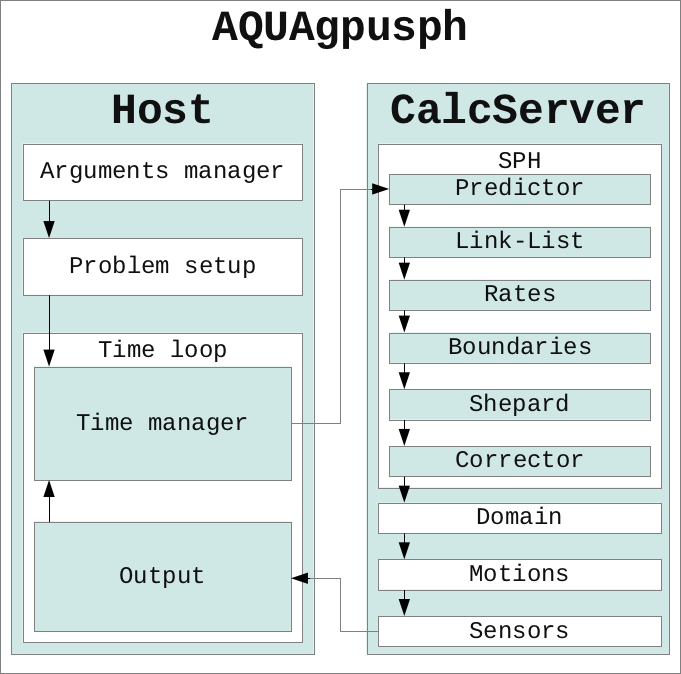
\includegraphics[width=0.7\textwidth]{GeneralDiagram}
  \caption{General \NAME flux diagram}
  \label{fig:aquagpusph:generalDiagram}
\end{figure}
%
\section{Arguments manager}
\label{ss:aquagpusph:argmanager}
%
Arguments manager is the piece of code that analyse input command line options/arguments. You can get a
list of valid options and arguments executing:
%
\begin{verbatim}
AQUAgpusph --help
\end{verbatim}
%
Valid options are:
%
\begin{itemize}
	\item \textbf{-i, -\--input=INPUT}: Set the definition XML file of the simulation.
	\item \textbf{-o, -\--output-prefix=PREFIX}: Set a prefix for output files.
	\item \textbf{-n, -\--no-reassembly}: Visualization output files will not reassembled.
	\item \textbf{-v, -\--version}: Show \NAME version and stop the execution.
	\item \textbf{-h, -\--help}: Show \NAME helps page and stop the execution.
\end{itemize}
%
Options can be freely used simultaneously until incompatibilities are not notified here, or at the help
page. Some combinations of command line options can result on undesired behaviour, like for instance
mixing -\--version with -\--help will discard one of them.\rc
%
In almost cases -\--no-reassembly is a good option, due to reassembly output files can be a really
hard-disk \& CPU consuming process.
%
\section{Problem setup}
\label{ss:aquagpusph:problemsetup}
%
The problem setup stage basically consist on loads all settings established as explained on chapter
\ref{s:caseSetup}, and load the particles/vertexes data from described files on chapter \ref{ss:partsFile}.\rc
%
Problem setup will report work done, and the eventually incidences, on the initialization screen output.
The screen output during initialization and close stages of \NAME execution will be preserved if NCurses
support has been activated, but if NCurses support is not active you can lost the initialization process
reported messages due to the large amount of these printed during the simulation. In this case you
can redirect the screen output to a file typing:
%
\begin{alltt}
AQUAgpusph \emph{COMMANDLINE_OPTIONS} > screen.out
\end{alltt}
%
You can also detach the execution from terminal, for instance using:
%
\begin{alltt}
nohup AQUAgpusph \emph{COMMANDLINE_OPTIONS} > screen.out &
\end{alltt}
%
Allowing you to run \NAME remotely, but in this case you will lost the possibility of stop simulation using `c'
key\footnote{Advanced Linux users can get the process PID and then reinject keys to program}, that as described
on chapter \ref{ss:running:launching} allows you to right stop the simulation closing files.\rc
%
In both cases you will preserve a file called ``screen.out'' that saves the messages reported during
initialization and close stages, and along the simulation as well.
%
\section{Leap-Frog integration scheme}
\label{ss:aquagpusph:leapfrog}
%
Weakly compressible SPH method is able to return the instantaneous acceleration and density rate for each
particle in a Lagrangian point of view, so 3 variables must be integrated along the time, velocity, position
and density of each particle. \NAME time integration is based on a Leap-Frog predictor-corrector scheme:
%
\begin{enumerate}
	\item Predictor:
	\[
	\dot x_{t+dt}^{\mathrm{pred}} = 
	\dot x_{t} + 
	dt \left(
		\ddot x_{t} + g
	\right)
	\]
	\[
	x_{t+dt}^{\mathrm{pred}} = 
	x_{t} + 
	dt \dot x_{t} + 
	\frac{dt^2}{2} \left(
		\ddot x_{t} + g
	\right)
	\]
	\[
	\rho_{t+dt}^{\mathrm{pred}} = 
	\rho_{t} + 
	dt \dot\rho_{t}
	\]
	\item SPH interactions:
	\[
	\ddot x_{t+dt} \leftarrow \mbox{SPH}
	\]
	\[
	\dot\rho_{t+dt} \leftarrow \mbox{SPH}
	\]
	\item Corrector:
	\[
	\dot x_{t+dt} = 
	\dot x_{t+dt}^{\mathrm{pred}} + 
	\frac{dt}{2} \left(
		\ddot x_{t+dt} - \ddot x_{t}
	\right)
	\]
	\[
	x_{t+dt} = x_{t+dt}^{\mathrm{pred}}
	\]
	\[
	\rho_{t+dt} = 
	\rho_{t+dt}^{\mathrm{pred}} + 
	\frac{dt}{2} \left(
		\dot\rho_{t+dt} - \dot\rho_{t}
	\right)
	\]
\end{enumerate}
%
\section{Link-List}
\label{ss:aquagpusph:linklist}
%
SPH codes commonly uses a PIC (Particle In Cell) based algorithm to easily locate particle's neighbours, called
Link-List. The main difference with typical PIC algorithm is that on SPH a chain is built from the cells data,
linking each particle with the next one on the same cell, allowing that cell only saves the index of the
first particle of the chain.\rc
%
In figure \ref{fig:aquagpusph:LinkList} a simplified scheme of Link-List stored data is shown. Particles are
located in cells that have a length of the maximum interaction distance, then each cell allocates a particle
index called ``head of chain'' (\textit{ihoc}). Each particle stores the next one of the cell chain (\textit{ll})
until last particle is reached, where some invalid index is set  (-1 for instance).\rc
%
In GPU oriented code this behaviour can be conveniently modified looking for sorted memory address reading, that
is really more efficient, sorting particles by cell index. The problem is that traditional method implies storing
Link-List chain, and more over, implies a chaotic memory access at particles interaction stage, with a heavy
performance penalty. So, as many other GPU based SPH codes, \NAME sorts the particles, transforming the Link-List
array ll[\textit{i}] in \textit{i}+1 variables, so is not anymore needed to store it therefore.\rc
%
\begin{figure}[h!]
  \centering
  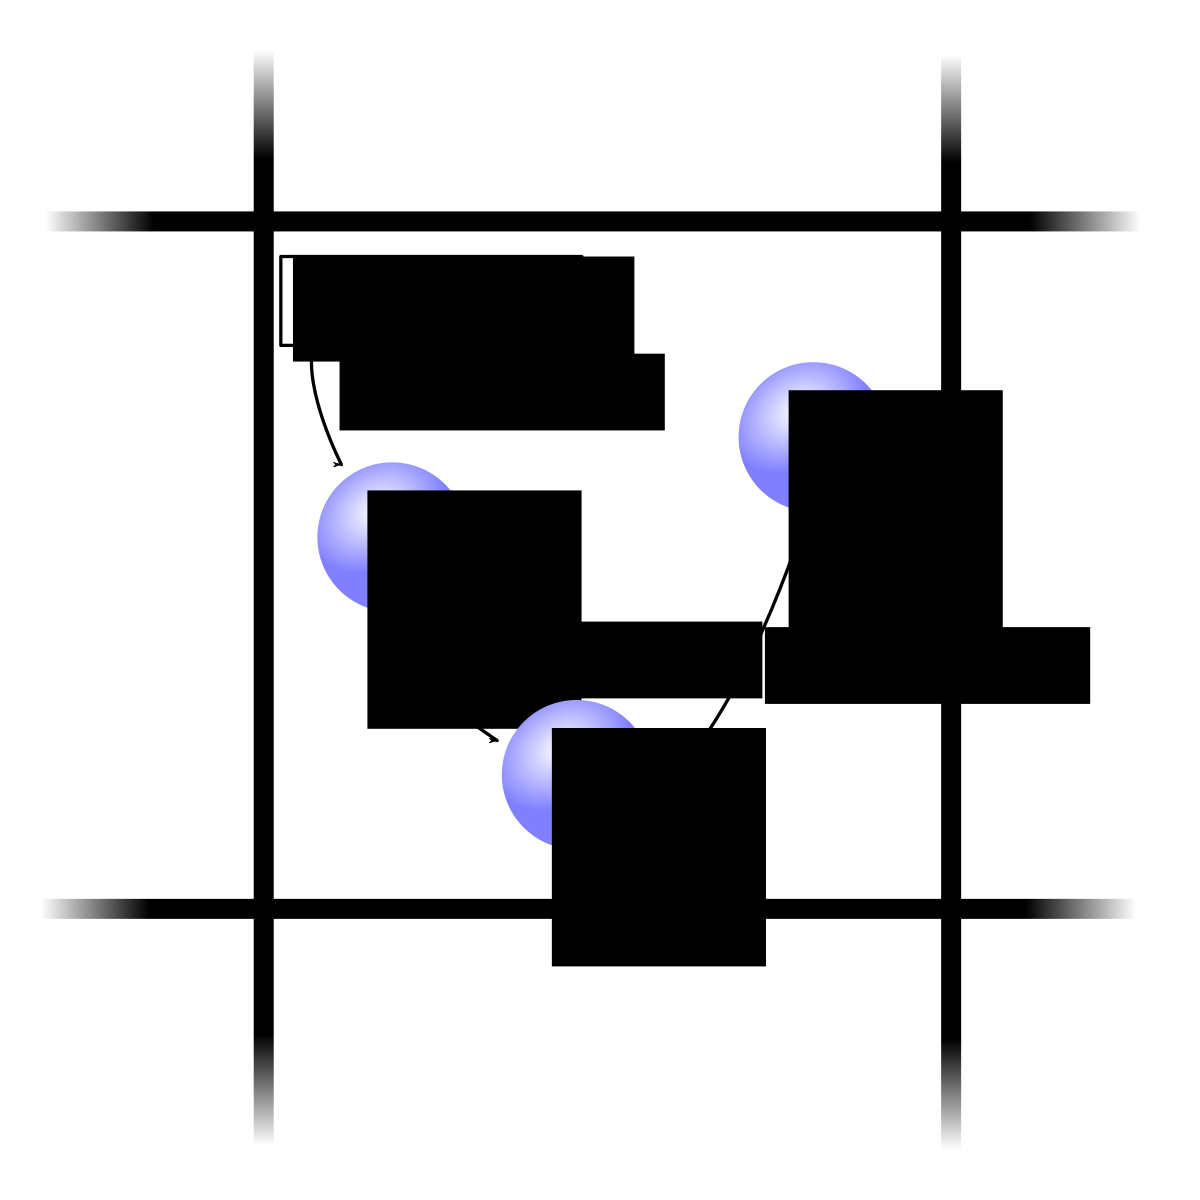
\includegraphics[width=0.7\textwidth]{LinkList}
  \caption{Conventional Link-List scheme}
  \label{fig:aquagpusph:LinkList}
\end{figure}
%
\section{Particles interactions}
\label{ss:aquagpusph:rates}
%
Particles interactions is the core of every SPH method, and is the most complex stage too, being the most
time consuming one. \NAME can perform several particles interaction stages by time step depending on simulation
settings, for instance, if `DeLeffe' boundary condition is set at least 3 interactions stages will be performed,
the usual one, the boundary integrals, and `ElasticBounce' non wall trespassing condition, but since only the usual one
needs to compute all possible particles interactions, the others may take less time.\rc
%
As explained in section \ref{ss:aquagpusph:linklist}, the particles interactions computation performance is
heavily dependant on Link-List stage and \NAME performs a particles sorting based on cell as many other GPU
oriented SPH codes, but two main differences must be remarked:
%
\subsection{Unsorted output arguments}
%
In section \ref{ss:aquagpusph:leapfrog} time integration scheme is described, and we can find that after predictor
stage, variables $\dot x_{t}$, $\mathbf{x}_{t}$, and $\rho_{t}$ are not needed anymore until new time step,
so \NAME can use these arrays in order to store sorted data for SPH interactions stage, decreasing memory
requirements, but the same process can not be applied to output data $\ddot x_{t}$ and $\dot\rho_{t}$,
because is needed on corrector stage, so there are 2 ways to solve it:
%
\begin{enumerate}
	\item Create new arrays for the sorted output data, working all time in sorted space.
	\item Work on sorted space, but write at unsorted space.
\end{enumerate}
%
\NAME use the second way, that have some significant advantages:
%
\begin{enumerate}
	\item Less memory requirements that the first way.
	\item Since \NAME is using non needed arrays to store the sorted input data, the unsorted data is preserved.
	\item Since the output data is written on unsorted space directly, after SPH interactions stage all the
	unsorted data is available to continue working, including to print output files (Note that the unsorted space
	is the original one).
	\item No unsort operation is required.
\end{enumerate}
%
Of course, write into the unsorted space at the interactions stage can be more expensive, but since the writing
operations are really less frequent than the reading ones, performance decrease can be assumed.
%
\subsection{Coalescence read}
%
Newest hardware not suffers really heavy penalties when a lot of threads try to read from the same memory address,
nevertheless \NAME incorporates an algorithm in order to reduce as much as possible the number of readers over
unique address. In figure \ref{fig:aquagpusph:CoalescenceRead} a scheme about the interactions process is shown.
Interactions stage is divided in 3 substages:
%
\begin{enumerate}
	\item Interacts with next particles of the home cell\footnote{Home cell is the cell where the computing
	particle is located} chain.
	\item Interacts with the particles on the neighbour cells.
	\item Interacts with previous particles of the home cell chain.
\end{enumerate}
%
As you can see in figure \ref{fig:aquagpusph:CoalescenceRead} the particles does not reads from the same memory
address in any interactions. In practice, due to the particles interactions can take different times, due to the
neighbour cells particles can try to read from same memory address, several simultaneous reads can happens, but
in much less number.
%
\begin{figure}[ht!]
  \centering
  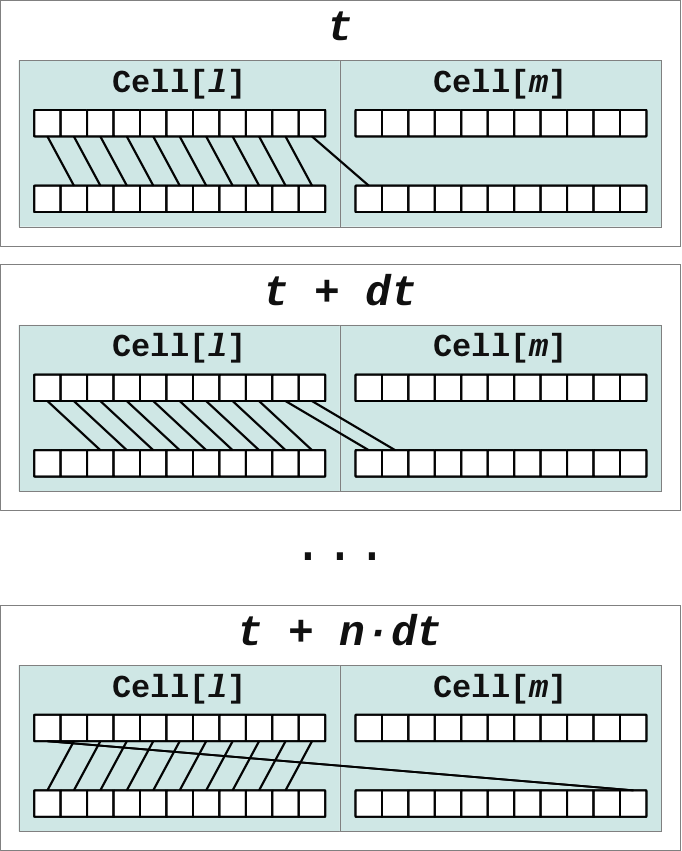
\includegraphics[width=0.7\textwidth]{CoalescenceRead}
  \caption{Coalescence reading flow}
  \label{fig:aquagpusph:CoalescenceRead}
\end{figure}
%
\section{Boundary conditions}
\label{ss:aquagpusph:boundaries}
%
\subsection{General}
%
\NAME provides most commonly used boundary conditions in order to allow users to can choose the one than better fit
to their problem. The generally suggested method is Boundary integrals (formerly `DeLeffe') that is flexible and
powerful, but have the disadvantage that requires `Shepard' correction for consistency.\rc
%
Along this chapter all boundary conditions will be described, and advantages discussed. Also the mixing possibilities
will be introduced.
%
\subsection{Elastic bounce}
\label{sss:aquagpusph:boundaries:elasticbounce}
%
This is the simplest way to impose the boundary conditions, based on particle elastic bound within the wall, where
a elastic factor is applied in order to set plasticity.\\
%
In figure \ref{fig:aquagpusph:BounceScheme} a scheme of the elastic bound effect is shown. In \NAME walls are
defined by a set of vertexes (black balls), that have a normal\footnote{Ensure yourself that the provided normals
are normalized, \NAME will accept it as set by user} and area associated (area is stored on mass array).
In order to \NAME identify particles as vertexes, $imove$ flag must be set lower than 0.\\
%
Elastic bounce is applied when a particle will moved nearer to a vertex than `BoundDist' parameter introduced on
chapter \ref{sss:XML:SPH}, then the normal component of velocity is modified in order to get an elastic bound
multiplied by elastic factor `BoundElasticFactor'. If the elastic factor is 1, a fully elastic bound will
performed, however if elastic factor is 0, particle will stopped (normal component of the velocity will affected
only), so with values between 0 and 1 a semi-elastic bound will performed. You can set elastic factors out of
[0,1] bounds if you know what are you doing.\\
%
Main advantage of this boundary is the simplicity that reverts on a good performance, but using the Elastic bounce
boundary condition alone will return poor physics results, The Elastic bounce boundary condition is then aimed to
work with other boundary conditions, serving a second barrier for particles that can try to trespass the walls.
%
\begin{figure}[h!]
  \centering
  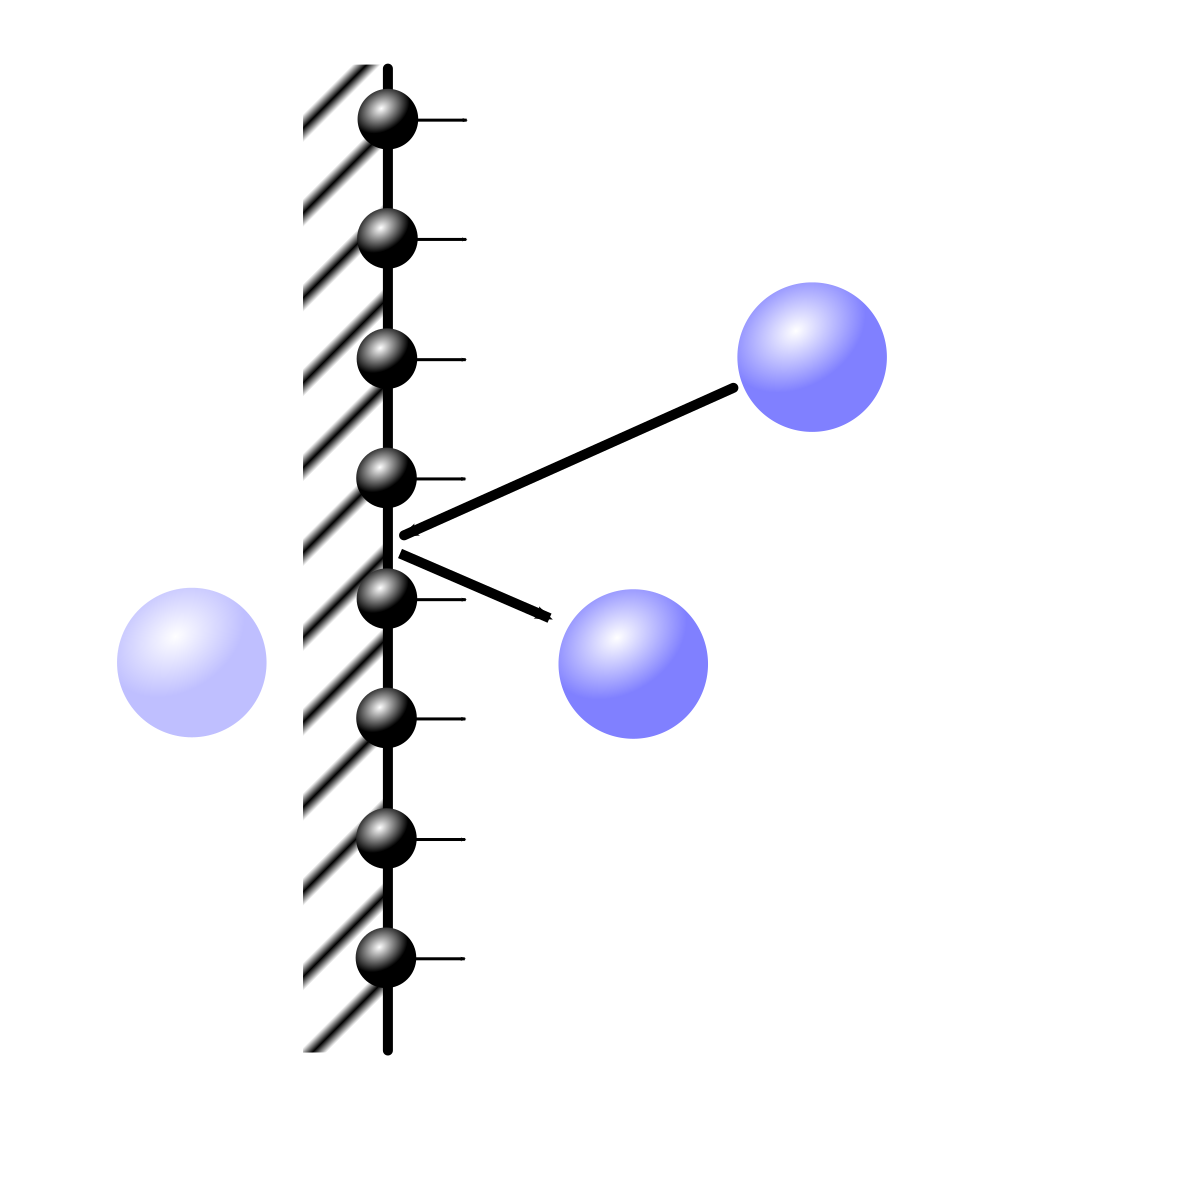
\includegraphics[width=0.25\textwidth]{ElasticBounce}
  \caption{Elastic bounce boundary scheme}
  \label{fig:aquagpusph:BounceScheme}
\end{figure}
%
\subsection{Fix particles}
\label{sss:aquagpusph:boundaries:fixparticles}
%
`Fix particles', also called `dummy particles' sometimes, is a extension of the fluid domain along walls with a little
bit especial fluid particles linked to them.\\
%
In figure \ref{fig:aquagpusph:FixParticlesScheme} an scheme of the fixed particles distribution is shown. Must be
noticed that first row of fixed particles is placed \textit{dr}/2 inner on wall, and the several rows are placed
every \textit{dr}. The fixed particles are similar to the fluid ones, but a normal must be provided and
\textit{imove} flag must be lower than 0.\\
%
The fixed particles will use continuity equation like the fluid particles, but not momentum equation, because
fixed particles velocity is linked to the wall motion. Related to this, if no motions are set, the initial fixed
particles velocity will be preserved along the simulation\footnote{you can modify this behaviour with custom
predictor and corrector kernels}.\\
%
SPH equations when `Fix particles' boundary condition is used are therefore
%
\[
\left. \left\langle \frac{\gradient p}{\rho} \right\rangle_a \right\vert_{a \in \mathrm{Fluid}} = \frac{1}{\gamma_a}
	\sum\limits_{b \in \mathrm{Fluid}\;\cup\;\mathrm{Boundary}} 
		\left( \frac{p_a}{\rho_a^2} + \frac{p_b}{\rho_b^2} \right)
	\gradient W_{ab} m_b
\]
%
\[
\left. \left\langle \rho \; \divergence(v) \right\rangle_a \right\vert_{a \in \mathrm{Fluid}\;\cup\;\mathrm{Boundary}} =
	- \frac{1}{\gamma_a}
	\sum\limits_{b \in \mathrm{Fluid}\;\cup\;\mathrm{Boundary}} 
		\left( v_a - v_b \right)
	\gradient W_{ab} m_b
\]
%
\[
v_{a \in \mathrm{Boundary}} = \mathrm{f}\left(x_\mathrm{walls} \left( t \right) \right)
\]
%
Where $\gamma_a$ can be forced to be 1 ever setting Shepard correction to ``None'' as decribed on the chapter
\ref{sss:XML:SPH}, that have the advantage of getting a fully conservative notation.\\
%
`Fix particles' uses internally `ElasticBounce boundary' condition described on section
\ref{sss:aquagpusph:boundaries:elasticbounce}. It's strongly recommended let `Fix particles' work with
`ElasticBounce boundary' in order to warranty that the particles can trespass the walls, but if you want to
disable this feature simply set `BoundDist' parameter to 0, \textbf{never pass null normals to the fixed
particles}.\\
%
`Fix particles' is chronologically the first boundary condition implemented on SPH, has the main advantage that is
easy to implement since the fixed particles have a really similar treatment to the usual fluid particles, but
have the main disadvantage of the particles velocity set using only walls motion as a `U0M', that gives an
inconsistent Laplacian operator. Also requires increase the number of particles significantly, more as the number of neighbours grows.
%
\begin{figure}[ht!]
  \centering
  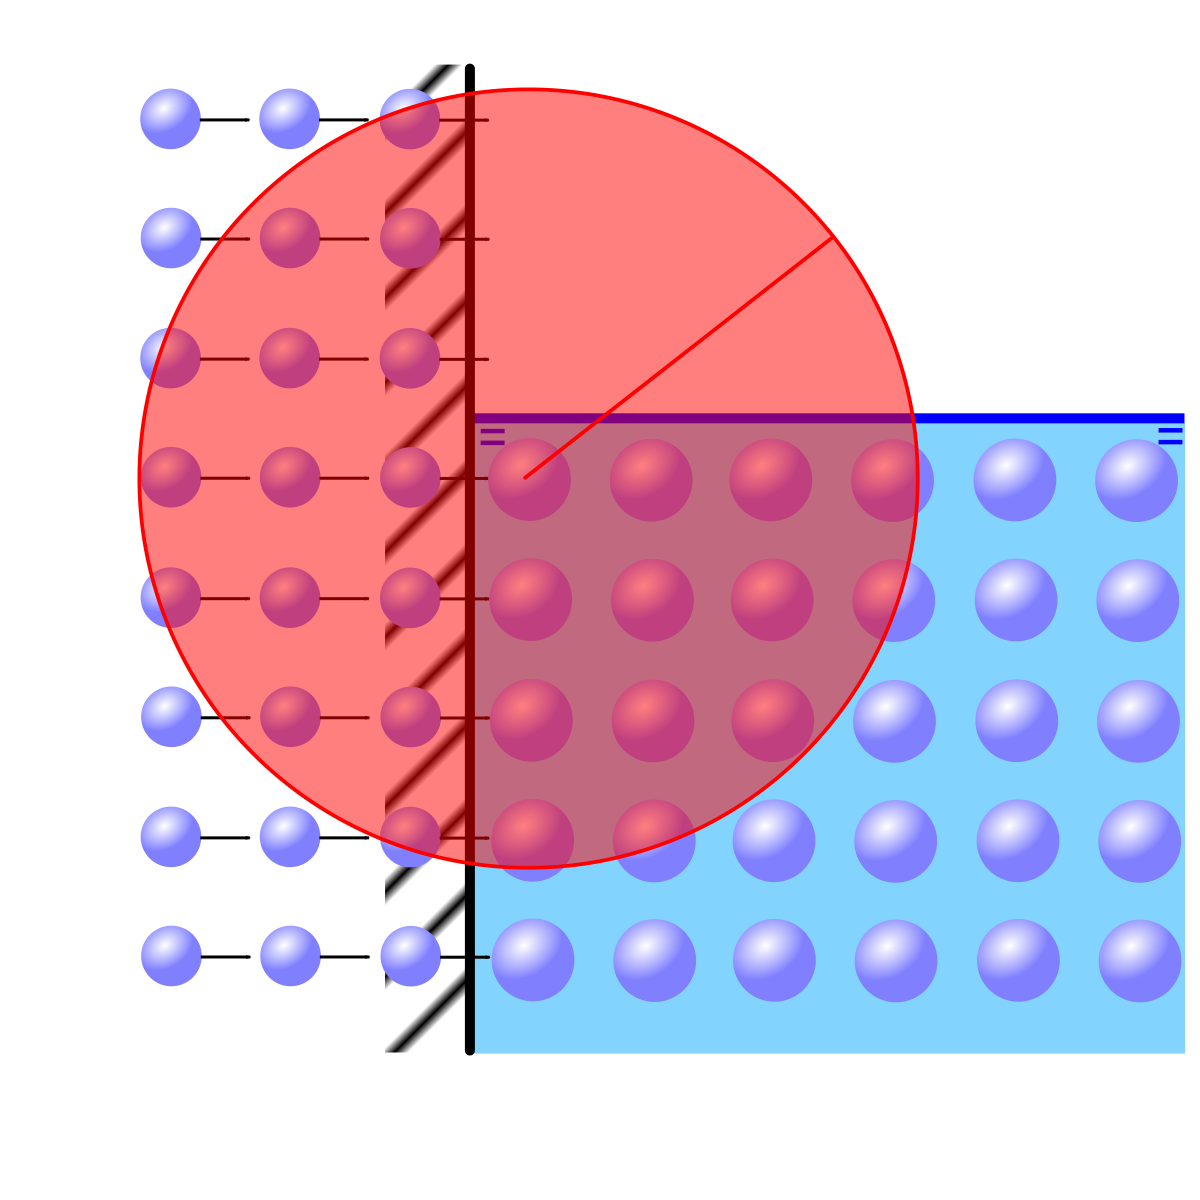
\includegraphics[width=0.4\textwidth]{FixedParticles}
  \caption{Fix particles scheme}
  \label{fig:aquagpusph:FixParticlesScheme}
\end{figure}
%
\subsection{Boundary integrals, formerly `DeLeffe'}
\label{sss:aquagpusph:boundaries:DeLeffe}
%
Boundary integrals is the newest method to compute boundary conditions, and the implementation method is similar
to `ElasticBounce boundary' described at section \ref{sss:aquagpusph:boundaries:elasticbounce}.\\
%
In figure \ref{fig:aquagpusph:DeLeffeScheme} a boundary integrals scheme is shown. In original DeLeffe's boundaries
integral development, oriented to 2D applications, an analytic solution of the integral, with a discretized
version of fields, is purposed for full integration line (green highlighted on the image). In \NAME each vertex
is associated to a wall area, then not only the field is discretized but also the integral as well, with a little
bit worst result, but allowing to use this method in 3D simulations too.\\
%
In order to can converge the discretized boundary integral to the analytical one, you can set more vertexes with
smaller areas, but be mindful that the values in vertexes along the walls are interpolated from the fluid particles,
so really high resolution in walls, compared to fluid resolution, don't make any sense due to bad interpolated
fields.\\
%
Boundary integrals have advantages in terms of consistency, with consistency of order $\mathcal{O}(h)$ for all the
operators, including the Laplacian. At the other hand this boundary condition requires Shepard correction, that
can be a little bit unstable, and breaks the fully conservative SPH notation. The equations are therefore
%
\[
\left. \left\langle \frac{\gradient p}{\rho} \right\rangle_a \right\vert_{a \in \mathrm{Fluid}} =
	\frac{1}{\gamma_a} \left(
		\sum\limits_{b \in \mathrm{Fluid}} 
			\left( \frac{p_a}{\rho_a^2} + \frac{p_b}{\rho_b^2} \right)
		\gradient W_{ab} m_b
		- \sum\limits_{b \in \mathrm{Boundary}}
			\rho_b \left( \frac{p_a}{\rho_a^2} + \frac{p_b}{\rho_b^2} \right)
		n_b S_b
	\right)
\]
\[
\left. \left\langle \rho \; \divergence(v) \right\rangle_a \right\vert_{a \in \mathrm{Fluid}} =
	- \frac{1}{\gamma_a} \left(
		\sum\limits_{b \in \mathrm{Fluid}} 
			\left( v_a - v_b \right)
		\gradient W_{ab} m_b
		- \sum\limits_{b \in \mathrm{Boundary}}
			\rho_b \left( v_a - v_b \right)
		n_b S_b
	\right)
\]
\[
p_{a \in \mathrm{Boundary}} = \sum\limits_{b \in \mathrm{Fluid}}
	\left( \frac{p_b}{\rho_b} + g \cdot r_{ab}\right )
	W_{ab} m_b
\]
\[
v_{a \in \mathrm{Boundary}} = \mathrm{f}\left(x_\mathrm{walls} \left( t \right) \right)
\]
%
Since the integration domain is truncated (this method is not based on a fluid extension), Shepard correction usage
is mandatory. In \NAME Shepard correction over the pressure term will be applied by default, but not over the
continuity equation, because compressibility is small in all cases, and Shepard correction can unstabilize this
equation. Nevertheless you can activate the Shepard normalization as described in the chapter \ref{sss:XML:SPH}.\\
%
Must be noticed that the vertexes must be placed on the center of their representative area, taking special care on
the limits of walls. In figure \ref{fig:aquagpusph:DeLeffeCorner} the distribution of vertexes, that is separated 
\textit{dr}/2 (half of distance between particles \textit{dr}), in a corner is shown. Since the area (line length
because is a 2D example) associated to each vertex is \textit{dr}/2, the distance of first vertex to corner is
\textit{dr}/4.\\
%
`DeLeffe' uses internally `ElasticBounce boundary' condition described on section
\ref{sss:aquagpusph:boundaries:elasticbounce}. It's strongly recommended let `DeLeffe' work with
`ElasticBounce boundary' in order to warranty that the particles can trespass the walls, but if you want to
disable this feature simply set `BoundDist' parameter to 0, \textbf{never pass null normals to the vertexes}.
%
\begin{figure}[h!]
  \centering
  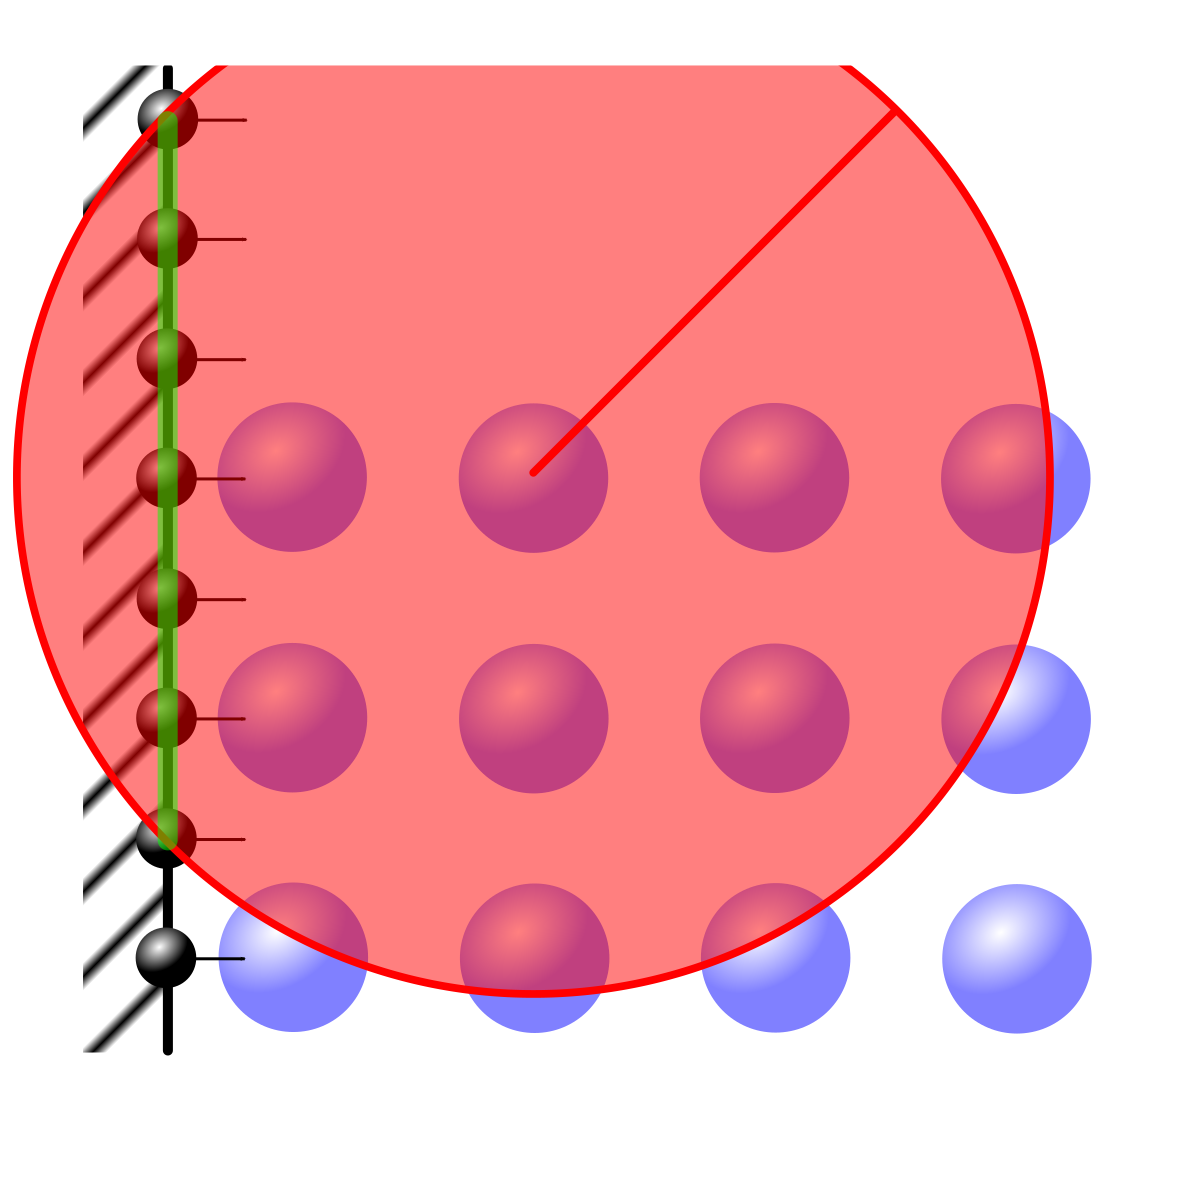
\includegraphics[width=0.4\textwidth]{DeLeffe}
  \caption{Boundary integrals scheme}
  \label{fig:aquagpusph:DeLeffeScheme}
\end{figure}
%
\begin{figure}[h!]
  \centering
  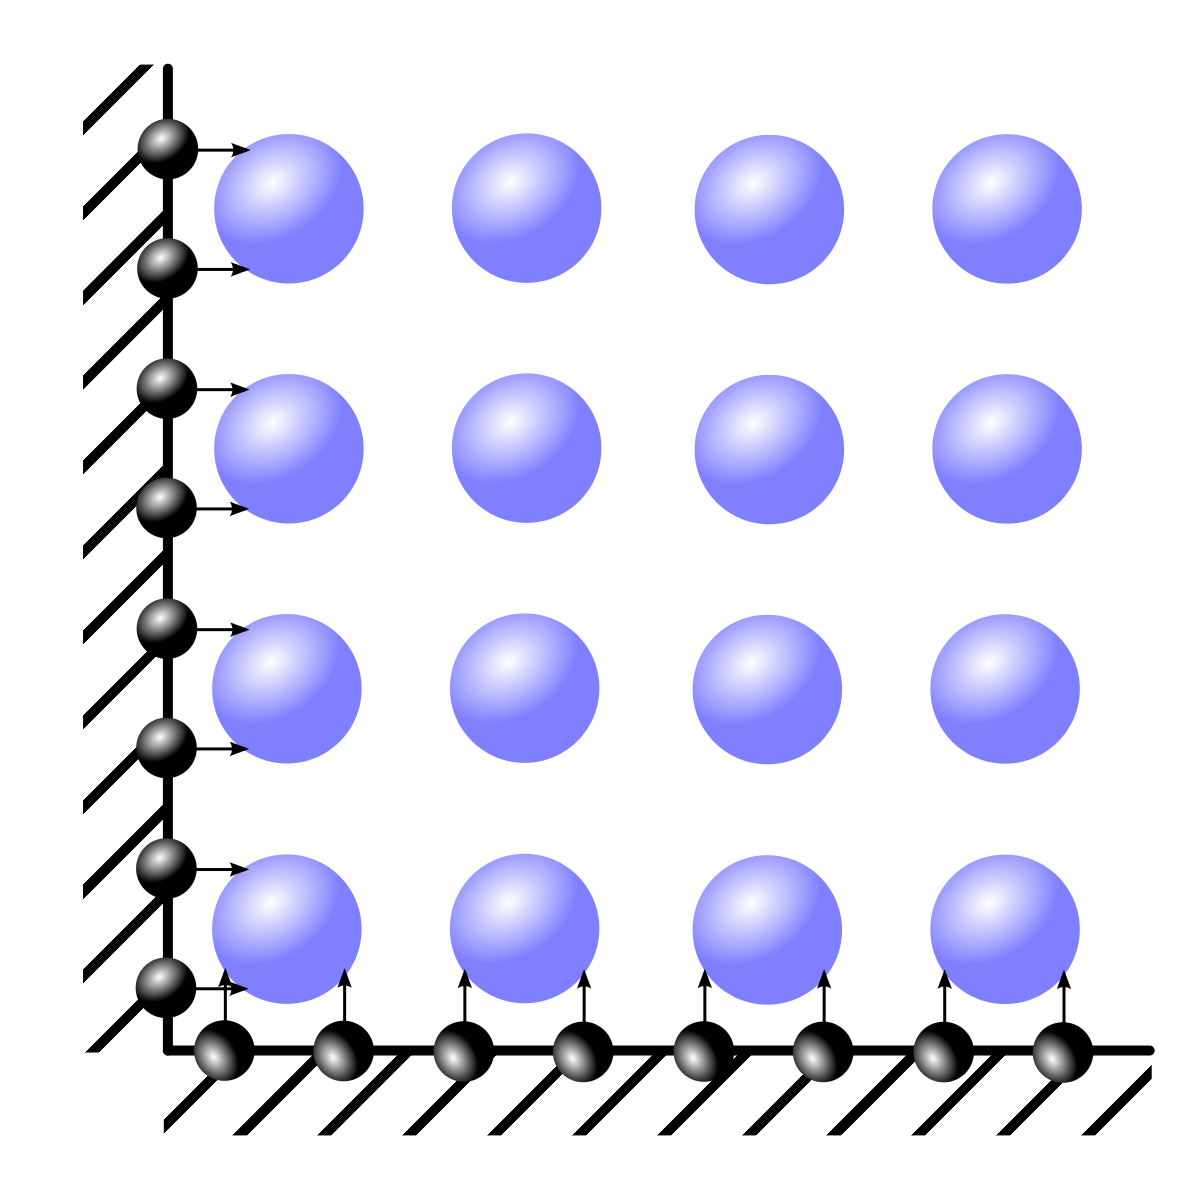
\includegraphics[width=0.4\textwidth]{DeLeffeCorner}
  \caption{Corner particles and vertexes distribution}
  \label{fig:aquagpusph:DeLeffeCorner}
\end{figure}
%
\subsection{Ghost particles}
\label{sss:aquagpusph:boundaries:ghostparticles}
%
`Ghost particles' is an algorithm so quite similar to `Fix particles' one, but in this case the extension of fluid
is not composed by particles linked to wall, that integrates their density using continuity equation, but is composed
by a mirroring of the fluid respect to the wall.\\
%
In the figure \ref{fig:aquagpusph:GhostParticlesScheme} a scheme about the fluid particles mirroring is shown.\\
%
So the SPH equation are therefore
%
\[
\left. \left\langle \frac{\gradient p}{\rho} \right\rangle_a \right\vert_{a \in \mathrm{Fluid}} = \frac{1}{\gamma_a}
	\sum\limits_{b \in \mathrm{Fluid}\;\cup\;\mathrm{Boundary}} 
		\left( \frac{p_a}{\rho_a^2} + \frac{p_b}{\rho_b^2} \right)
	\gradient W_{ab} m_b
\]
\[
\left. \left\langle \rho \; \divergence(v) \right\rangle_a \right\vert_{a \in \mathrm{Fluid}} =
	- \frac{1}{\gamma_a}
	\sum\limits_{b \in \mathrm{Fluid}\;\cup\;\mathrm{Boundary}} 
		\left( v_a - v_b \right)
	\gradient W_{ab} m_b
\]
\[
p_{a \in \mathrm{Boundary}} = \mathrm{f}\left(x_a, x_\mathrm{walls} \left( t \right) \right)
\]
\[
v_{a \in \mathrm{Boundary}} = \mathrm{f}\left(x_a, x_\mathrm{walls} \left( t \right) \right)
\]
%
The usual method to implement this boundary condition is perform a mirroring stage before the particles interaction,
storing the mirrored particles data in order to can use them within the fluid particles integration. In GPU
oriented code\footnote{and more generally for any parallel oriented one} this approach has the problem of the
previously unknown number of ghost particles, so memory reallocation or over-dimensioned arrays are mandatory
therefore. This can be walked around creating fix particles, but getting their values from fluid by a mirroring
operation and interpolation, with the advantage that the number of particles is ever know and reallocation is not
needed therefore, but with the disadvantage that requires to generate the fixed particles.\\
%
In \NAME a new algorithm is drafted, where the ghost particles are not precomputed, called `Virtual ghost particles'.
With this method a particles interaction process is called for each wall defined, so this method is not recommended
to high number of walls, nevertheless, when the particles interaction is called respect to a wall, each particle will
first test that is enough near to the wall before start working, so each `Ghost particles' interaction called is
significantly cheaper than usual one. The working method is locate all neighbours of the particle as is done on the
usual particles interaction method, and for each neighbour located compute the mirrored particle on runtime, avoiding
the need to store this data.\\
%
Since the number of walls must be relatively small, define the walls using particles with $imove < 0$ flag is not a
good option, so \NAME provides a parallel interface as has been described on chapter \ref{sss:XML:GhostParticles}.
This feature allows you to mix `Ghost particles' boundary condition with all other previous described, but probably
you only wants to mix it with `ElasticBounce boundary', in order to ensure than the fluid particles will not trespass
the walls.\\
%
`Ghost particles' boundary has the advantages of be easily defined in simple cases, and has been widely employed
along the SPH method history, so results can be easily compared. `Ghost particles' have some consistency problems
and is a condition bad defined in corners. When walls are perpendiculars the problem can be walked around adding
diagonal walls as shown in figure \ref{fig:aquagpusph:GhostParticlesCorner}, but for the moment general angles
intersection can not be solved in \NAME with `Ghost particles' boundary method yet.
%
\begin{figure}[h!]
  \centering
  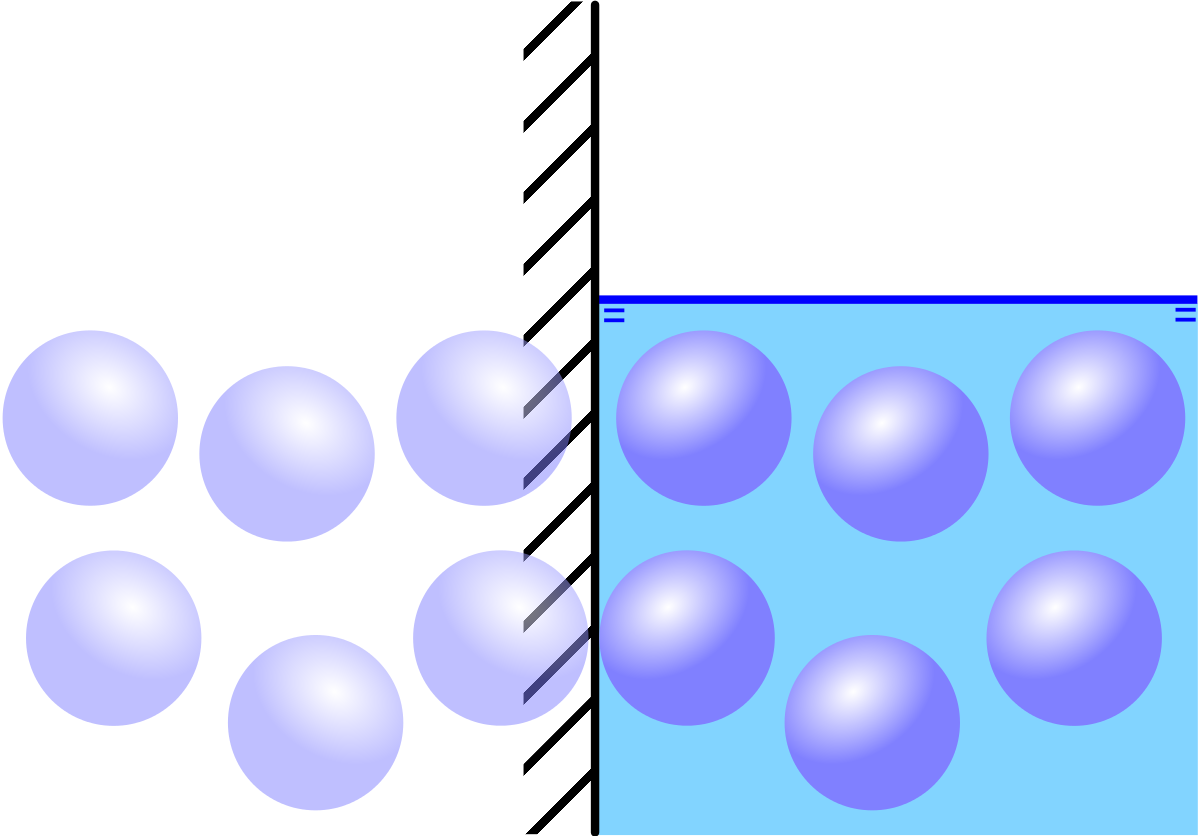
\includegraphics[width=0.4\textwidth]{GhostParticles}
  \caption{Ghost particles scheme}
  \label{fig:aquagpusph:GhostParticlesScheme}
\end{figure}
%
\begin{figure}[ht!]
  \centering
  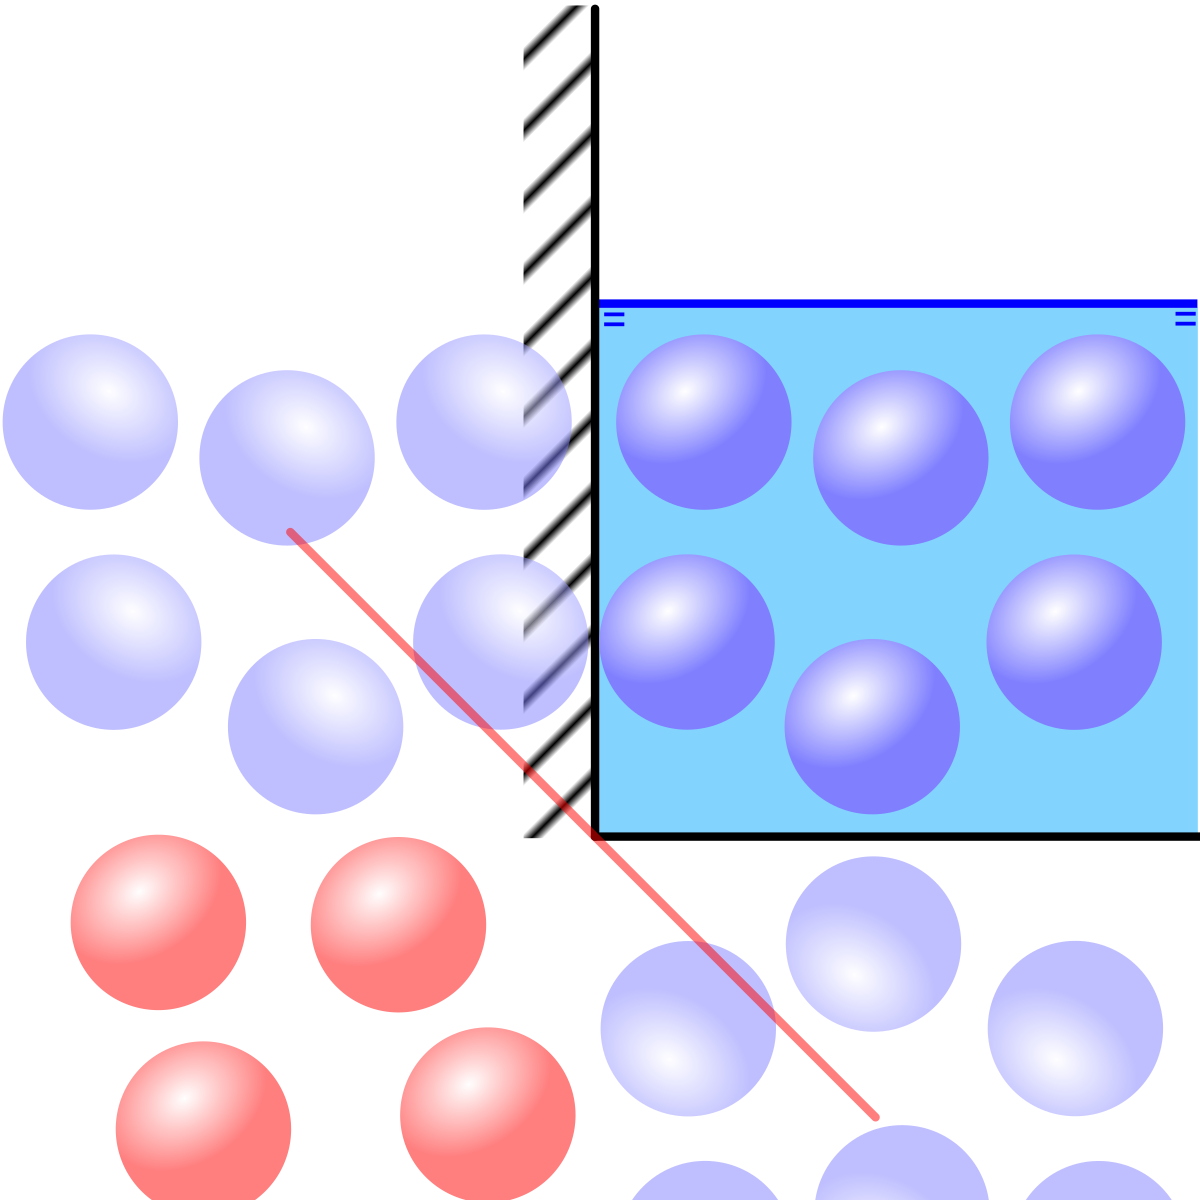
\includegraphics[width=0.4\textwidth]{GhostParticlesCorner}
  \caption{Ghost particles corner distribution}
  \label{fig:aquagpusph:GhostParticlesCorner}
\end{figure}
%

%
\section{Motions}
\label{ss:aquagpusph:motions}
%
\subsection{General}
%
In \NAME the motions imposed externally can be classified in 2 ways, by the method to impose the motion, and
by the method to compute the motion data. In table \ref{tables:aquagpusph:motions} all the available motions
in \NAME are listed, with their classification.\rc
%
Along this section all the different motion types, and control methods will be described. You can go to the
chapter \ref{s:examples} to see practical applications of some number of available motions.
%
\begin{table}[h!b!p!]\small
	\centering
	\begin{tabular}{| c | c | c | l | }
		\hline
		\cellcolor[rgb]{0.7,0.7,0.7}Movement & \cellcolor[rgb]{0.7,0.7,0.7}Motion type & \cellcolor[rgb]{0.7,0.7,0.7}Computation method \\
		\hline
		LIQuaternion     & Quaternion defined by axes & Linear interpolated data table \\
		\hline
		ScriptQuaternion & Quaternion defined by axes & Python script \\
		\hline
	\end{tabular}
	\caption{\NAME available motions.}
	\label{tables:aquagpusph:motions}
\end{table}
%
\subsection{Motion types}
\label{sss:aquagpusph:motions:Types}
%
\begin{center}
\textbf{Quaternion based motions}
\end{center}
%
The main method to impose motions in \NAME is to use Quaternions, that have the key feature that the motion is
ever fully described, not depending on any criteria. The problem with Quaternion imposed motions is that will
overwrite all the previous motions, so if you want to superpose several motions, Quaternion one must be the first.\\
%
When Quaternion motion is imposed in reality you are setting a movable reference coordinates, where object is fixed,
So in order to define instantaneous quaternion you must provide enough data to can describe it.
%
\begin{enumerate}
	\item 2D Simulations (AQUAgpusph2D)
	\begin{enumerate}
		\item \textbf{C.x}: x coordinate of the quaternion center.
		\item \textbf{C.y}: y coordinate of the quaternion center.
		\item \textbf{X.x}: x component of the X quaternion axis.
		\item \textbf{X.y}: y component of the X quaternion axis.
	\end{enumerate}
	\item 3D Simulations (AQUAgpusph)
	\begin{enumerate}
		\item \textbf{C.x}: x coordinate of the quaternion center.
		\item \textbf{C.y}: y coordinate of the quaternion center.
		\item \textbf{C.z}: z coordinate of the quaternion center.
		\item \textbf{X.x}: x component of the X quaternion axis.
		\item \textbf{X.y}: y component of the X quaternion axis.
		\item \textbf{X.z}: z component of the X quaternion axis.
		\item \textbf{Y.x}: x component of the Y quaternion axis.
		\item \textbf{Y.y}: y component of the Y quaternion axis.
		\item \textbf{Y.z}: z component of the Y quaternion axis.
	\end{enumerate}
\end{enumerate}
%
The undefined axis will be computed considering an orthonormal base. Provided axes will not be normalized, so
please ensure to provide right axes data.\\
%
Quaternion motions provided in \NAME will apply the motion over the particles with $imove \le 0$ flag (Fixed
particles or vertexes) and over defined walls as described on section \ref{sss:XML:GhostParticles}. You can
customize affected motion particles editing the provided Quaternion OpenCL kernel, but not walls for `Ghost
particles' boundary condition, that requires editing the \NAME source code.\\
%
In almost SPH simulations the time step is really small, for this reason in \NAME the velocity of the boundary
points (fixed particles, vertexes, or wall points) is determined as an euler derivation
%
\[v_{t+dt} = \frac{x_{t+dt} - x_t}{dt}\]
%
\subsection{Computation methods}
\label{sss:aquagpusph:motions:Controls}
%
\begin{center}
\textbf{Linear interpolated data table}
\end{center}
%
The simplest method to set the motion data is providing a tabulated file with the required data (see section
\ref{sss:aquagpusph:motions:Types} to know what data is required by the selected motion). Tabulated file
must contain one line per time instant with time at first column, and all the request fields by motion at the next
ones.\\
%
Comments can be included in the file with the symbol '\#'. All the line content after '\#' symbol will be
ignored. Fields can be separated by comma, semicolon, parenthesis, spaces or tabulator symbols, and if several
separators are concatenated between the field values then will be joined as a unique space separator.\\
%
When values are requested for a time instant $t$, such that $t_n < t < t_{n+1}$, values will be linearly interpolated
%
\[x(t) = \frac{t - t_n}{t_{n+1}-t_n} x(t_{n+1}) + \left( 1 - \frac{t - t_n}{t_{n+1}-t_n} \right) x(t_n)\]
%
You can see the section \ref{s:examples} to see practical application of linear interpolated tabulated motions data.
%
\begin{center}
\textbf{Python script controlled motion}
\end{center}
%
The most flexible and powerful method to control the motion is using a Python script where 2 methods must be
implemented:\\
%
\underline{\textbf{init}}\\
%
Method used to give the needed fields, as described on section \ref{sss:aquagpusph:motions:Types} for each type of
motion, for the time instant $t = 0 \mathrm{s}$, that can be useful to set initial condition.\\
%
\underline{\textbf{perform}}\\
%
Method called each time step in order to get all needed fields, as described on section
\ref{sss:aquagpusph:motions:Types} for each type of motion.
%
Input and output arguments may vary for both methods depending on the type of motion selected. We really encourage
user to go to chapter \ref{s:examples}, where practical applications of Python controlled motions can be found.
%
%
\section{Sensors}
\label{ss:aquagpusph:sensors}
%
In \NAME sensors are points where pressure and density fields will be measured. The method to add sensors into
the simulations has been described in the section \ref{sss:XML:Sensors}.\rc
%
Internally, the sensors are set as particles similar to the fluid ones, but with $imove = 0$ flag (fluid particles
have $imove > 0$ flag, and solid boundary elements $imove < 0$), and a null mass. The fields are interpolated in
the way described in section \ref{ss:sph_description}, where the discretized operators can be defined such that
%
\begin{eqnarray}
\label{eq:sensors:interpolation}
\langle p \rangle_a & = & \frac{1}{\gamma_a} \sum\limits_{b \in \mathrm{Fluid}} \frac{p_b}{\rho_b} W_{ab} m_b
\vspace{0.3cm} \\
\langle \rho \rangle_a & = & \frac{1}{\gamma_a} \sum\limits_{b \in \mathrm{Fluid}} W_{ab} m_b
\end{eqnarray}
%
Sensors measured values are ever renormalized with the Shepard correction ($\gamma_a$ is not forced to be equal to
1), even though Shepard correction has switched off for the forces and density rate computation, but in order to
you can revert the correction $\gamma_a$ (formerly $sumW$) is included into the output sensors data file.\rc
%
The sensors output data file is printed in the execution folder (so enough permissions are expected) with the name
``\textbf{Sensors.dat}'', inside the file a header will be printed, where the fields included are documented, and
then several rows (one per output time instant) with the following data distributed in columns:
%
\begin{enumerate}
	\item Time instant $t \mbox{[s]}$.
	\item Sensor data columns (one per sensor).
	\begin{enumerate}
		\item X position  $X \mbox{[m]}$.
		\item Y position  $Y \mbox{[m]}$.
		\item Z position  $Z \mbox{[m]}$ (only for 3D cases).
		\item Pressure $p \mbox{[Pa]}$.
		\item Density $\rho \mbox{[kg/m}^3\mbox{]}$.
		\item Kernel completeness factor $\gamma$.
	\end{enumerate}
\end{enumerate}
%
The fields are separated by tabulators. This file can be directly plot with gnuplot, or loaded easily with almost
data sheets.
%
%


% -------------------------------
% Examples
% -------------------------------
\chapter{Examples}
\label{s:examples}
%
\section{General}
%
In this section the examples provided with the \NAME package are documented, introducing the most intelligible
way to generate the case, the method to running it, and the post-process applied. \rc
%
Some examples are based on papers, or has been used in some publications, that are conveniently documented in
order to you can refer it if you want to learn more about the cases basis.
%
\section{Lateral water impact 1x, with De Leffe boundary condition}
\label{ss:example:lateral_water_1x_deleffe}
%
\subsection{General}
%
This case is based on \citet{botia_etal_spheric10}, where experimental data is available. This experiment has
been simulated in \NAME and published in \citet{Maciaetal_PTP_2012}. As menitoned in source paper, you can get
all the experiment data from \url{http://canal.etsin.upm.es/ftp/SPHERIC\_BENCHMARKS}. Here we will perform a
relaxed version of the simulation published.
%
The topics that will be covered in this example are:
%
\begin{enumerate}
	\item How to setup a physical model, with some subtopics:
	\begin{enumerate}
		\item How to setup default \NAME solver for the Navier-Stokes equations (See section \ref{s:model}).
		\item How to setup a domain.
		\item How to setup De Leffe boundary condition.
		\item How to setup a linear interpolated quaternion motion.
	\end{enumerate}
	\item How to discretize the domain.
	\item How to discretize the time.
	\item How to run and track a simulation.
	\item How to plot output data with gnuplot.
	\item How to visualize output with Paraview.
\end{enumerate}
%
This example is related with the next one, where the same experiment is simulated but ghost particles boundary
condition is used instead of boundary integrals one.\rc
%
In order to get a ready to run instance of this example 2D, version of \NAME package must be built, and examples
must be switched on at CMake configuration, as described in section \ref{sss:install:cmake}. You can find the
example either on the built package, at the subfolder ``examples'', and on the installed package, at\\
``\$\{CMAKE\_INSTALL\_PREFIX\}/\$\{CMAKE\_INSTALL\_DATADIR\}/examples'' (see section \ref{sss:install:cmake} to
learn more about this folder).\rc
%
In this example we will build the case from the scratch, creating all the files required manually, aiming to
a more illustrative process, but usually you don't want to follow this way and you may consider to use
previously generated cases and edit them. Following examples will be performed in a more practical way.
%
\subsection{Case description}
\label{sss:example:lateral_water_1x_deleffe:caseDescription}
%
The test is focused on a wave impact problem, being a rectangular tank with a roll forced motion, where pressures
along the time are registered in specific locations. The main objective is reproduce the wave impact pressure
registered.\rc
%
In the figure \ref{fig:examples:lateral_water_1x_deleffe_scheme:scheme} a schematic view of the tank with the
dimensions and sensors placed is shown. The thickness of the tank is 62mm, and is filled with 93mm of water.
In the scheme the rotation center is shown as well.\rc
%
In the figure \ref{fig:examples:lateral_water_1x_deleffe_scheme:press} the pressure registered on sensor 1
along the experiment is shown, with the roll forced motion. Must be noticed that the forced motion is almost a
sinusoidal motion but for the initialization stage. The most relevant impact is the first one, being the main
objective to simulate.\rc
%
Since the thickness of the tank is small compared with the other dimensions, and Reynolds number high due to the
water fluid usage, the effect on direction perpendicular to paper is neglected, considering a 2D case.
%
\begin{figure}[h!]
  \centering
  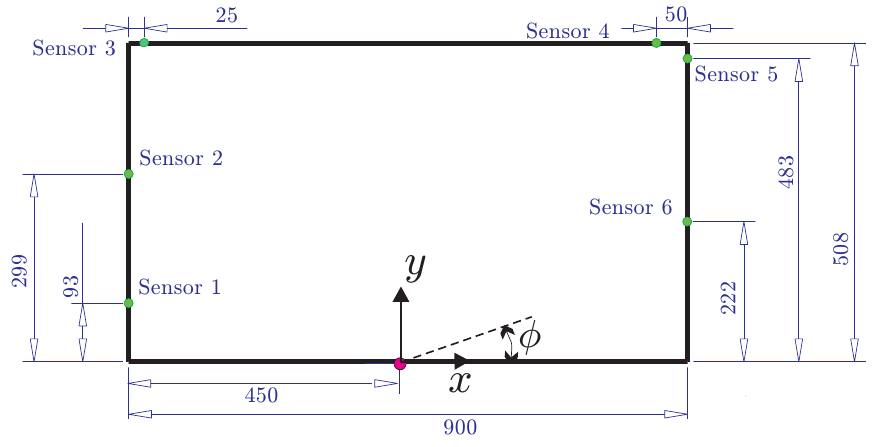
\includegraphics[width=0.8\textwidth]{lateral_water_1x_deleffe/tank}
  \caption{Tank dimensions and sensor positions}
  \label{fig:examples:lateral_water_1x_deleffe_scheme:scheme}
\end{figure}
%
\begin{figure}[h!]
  \centering
  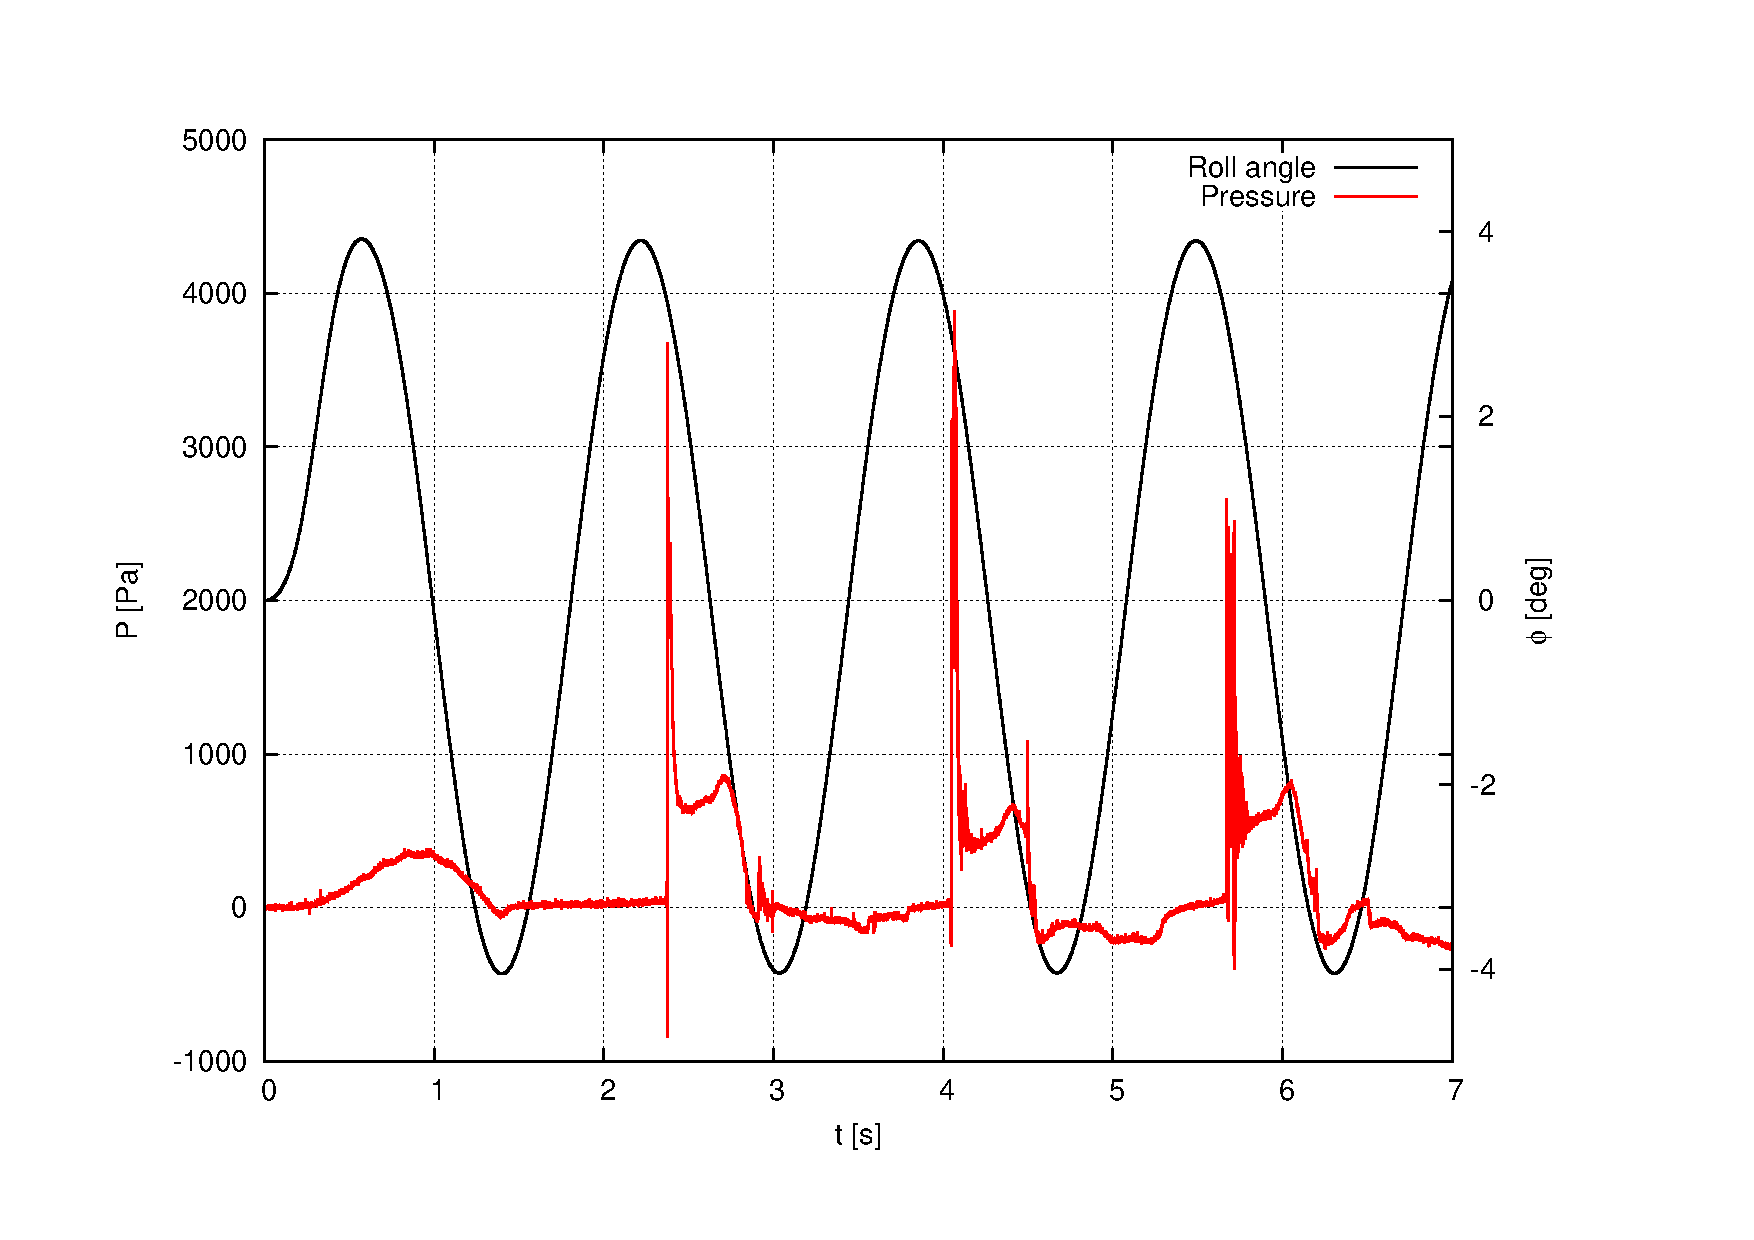
\includegraphics[width=0.9\textwidth]{lateral_water_1x_deleffe/press}
  \caption{Pressure registered on sensor 1, and the motion registry}
  \label{fig:examples:lateral_water_1x_deleffe_scheme:press}
\end{figure}
%
\subsection{Creating folder and files}
%
We will use a similar folder and files structure than the used on the provided example with the \NAME package.
First generate the folder when do plain to work (hereinafter \$EXAMPLE\_PATH), and into the folder generate
2 additional subfolders:
%
\begin{enumerate}
	\item \textbf{doc}: We will place here some files needed to plot the output data.
	\item \textbf{Move}: We will place here all the motions data, including the description XML file.
\end{enumerate}
%
Then go to the \href{http://canal.etsin.upm.es/ftp/SPHERIC\_BENCHMARKS}{benchmark web page} in order to download
the file ``lateral\_water\_1x.txt''\footnote{You can get this from the example provided with the package too}.
This file contains the experimental data, so place it in the ``doc'' subfolder.\rc
%
Now we are ready to start setting up the case data. For practical purposes hereinafter we will consider that \NAME
has been installed using following options (almost of them are the default options):
%
\begin{verbatim}
AQUAGPUSPH_3D             = OFF
AQUAGPUSPH_BUILD_DOC      = OFF
AQUAGPUSPH_BUILD_EXAMPLES = ON
CMAKE_INSTALL_PREFIX      = /usr
CMAKE_INSTALL_BINDIR      = bin
CMAKE_INSTALL_DATADIR     = share/aquagpusph
CMAKE_INSTALL_DOCDIR      = share/doc/aquagpusph
CMAKE_INSTALL_INCLUDEDIR  = include/AQUAgpusph
CMAKE_INSTALL_LIBDIR      = lib
\end{verbatim}
%
So resources have been installed into ``/usr/share/aquagpusph/resources'' folder. Also you can find the examples
resources (sources and scripts) in the folder ``/usr/share/aquagpusph/examples'', please refer to it in order to
see the final resulting configuration files.
%
\subsection{Setting physical model}
%
\subsubsection{General}
%
Several XML files will be created now, so hereinafter, if not any other indication is present, we will assume that
when a new XML file is created, this content will be included by default:
%
\begin{verbatim}
<?xml version="1.0" ?>
<sphInput>
</sphInput>
\end{verbatim}
%
Where we will insert data between ``sphInput'' tags.\rc
%
Physical model will be distributed in several sections:
%
\begin{enumerate}
	\item \textbf{Equations to solve}: \NAME allows you to set the OpenCL codes that will be used to perform
	the simulations, allowing to change the equations to solve as well.
	\item \textbf{Domain}: Domain related data, i.e. computational domain, gravity acceleration, fluids
	properties, corrections, ...
	\item \textbf{Boundary conditions}: Type of boundary condition used, no-slip/free-slip condition, ...
	\item \textbf{Movements}: Motions description.
\end{enumerate}
%
The data of these physical model sections are distributed in several files. You can refer to chapter
\ref{s:caseSetup} to know in detail the place where data must be allocated.\rc
%
\subsubsection{Equations to solve}
\label{sss:example:lateral_water_1x_deleffe:equations}
%
We will set the standard \NAME solver that is described in chapter \ref{s:model}, so we will set the OpenCL codes
provided with \NAME package. Create a XML file called ``\textbf{OpenCL.xml}'', with a section called ``OpenCL'',
and add into the default OpenCL code files. Finally you may get a file similar to this one:
%
\begin{verbatim}
<?xml version="1.0" ?>
<sphInput>
	<OpenCL>
		<Predictor file="/usr/share/aquagpusph/resources/OpenCL/Predictor" />
		<LinkList file="/usr/share/aquagpusph/resources/OpenCL/LinkList" />
		<Rates file="/usr/share/aquagpusph/resources/OpenCL/Rates" />
		<Corrector file="/usr/share/aquagpusph/resources/OpenCL/Corrector" />
		<TimeStep file="/usr/share/aquagpusph/resources/OpenCL/TimeStep" />
		<Reductions1D file="/usr/share/aquagpusph/resources/OpenCL/Reductions1D" />
		<Reductions file="/usr/share/aquagpusph/resources/OpenCL/Reductions" />
		<RadixSort file="/usr/share/aquagpusph/resources/OpenCL/RadixSort" />
		<Shepard file="/usr/share/aquagpusph/resources/OpenCL/Shepard" />
		<Domain file="/usr/share/aquagpusph/resources/OpenCL/Domain" />
		<ElasticBounce file="/usr/share/aquagpusph/resources/OpenCL/Boundary/ElasticBounce" />
		<DeLeffe file="/usr/share/aquagpusph/resources/OpenCL/Boundary/DeLeffe" />
	</OpenCL>
</sphInput>
\end{verbatim}
%
Note that OpenCL code file extension is automatically append. In the provided example this file has been replace by
a general version provided with \NAME package that you can find in
``/usr/share/aquagpusph/resources/OpenCLMain.xml'' path.
%
\subsubsection{Domain}
%
First for all we will set the domain fields, to do that we will generate a XML file called ``\textbf{SPH.xml}'' with
a section called ``SPH''. The fields that we want to set are:
%
\begin{enumerate}
	\item $\bs{g}$: Is the gravity acceleration. if you want to define other volumetric forces you can do it, as
	an acceleration unless you set you own mod \NAME version (see section
	\ref{sss:example:lateral_water_1x_deleffe:equations}). Since this is a 2D simulation this field must have 2
	components.
	\item $c_s$: Sound speed. Is a specific fluid property, but in weakly compressible SPH this value is really
	relevant on global properties, like the time step, \NAME needs a global value set. Usually this value is
	significantly lower than the real one.
	\item $\gamma$: Batchelor' 67 state equation exponent. Is a specific fluid property, but if some fluid has this
	property undefined, this value will used. 
\end{enumerate}
%
To do it add following \textit{Options}:
%
\begin{verbatim}
<Option name="g" x="0.0" y="-9.81" />
<Option name="gamma" value="1.0" />
<Option name="cs" value="45.0" />
\end{verbatim}
%
Also you can set what corrections will be applied on the simulation:
%
\begin{enumerate}
	\item \textbf{Steps between Link-List steps}: Link-List is a little bit time consuming stage, so don't
	preforming this operation each time step you can win some speed-up, but increasing the time steps between
	Link-List implies increasing the cells heigh, so more neighbours per particle will computed, and
	computational time increased, so take care with this value. In this example we will set that Link-List will
	performed each time step.
	\item \textbf{Density reinitialization}: Due to the compressibility the density and pressure fields can turn
	too noisy along the simulation, but you can interpolate the density field from the particles positions data.
	Be mindful that density reinitialization can carry some instabilities. In this example we will unset the
	density reinitialization (setting 0 as the steps between reinitializations).
	\item \textbf{Shepard}: See section \ref{ss:sph_continuous} to learn more about the renormalization factor.
	Renormalization factor is a correction that can improve some mathematics properties of the interpolation,
	however, using it the fully conservation formulation is broken, that is a missed feature. At the other hand
	Shepard correction is mandatory when boundary integrals is imposed as the boundary condition, so in this
	case we may activate it, but in order to set the simulation as many robust as possible, we will only apply
	Shepard correction for forces computation, but not for density rate (Shepard at density rate increase the
	the compressibility and the noisy density field therefore).
\end{enumerate}
%
Additionally, we will set a computable domain. The particles that go out the computable domain will be replaced
by a particle with null mass, and the motion flag conveniently changed to $imove = 0$ (a sensor). If you don't
set a computable domain, infinite domain will considered, but in this case, if one or more particles goes too
far (go out from tank in this example) the simulation may crash because the number of cells can be greater than
the allocatable one.\rc
%
After the changes your file may looks like this (later we will append more data to this file):
%
\begin{verbatim}
<?xml version="1.0" ?>
<sphInput>
	<SPH>
		<Option name="g" x="0.0" y="-9.81" />
		<Option name="gamma" value="1.0" />
		<Option name="cs" value="45.0" />
		<Option name="LLSteps" value="1" />
		<Option name="DensSteps" value="0" />
		<Option name="Shepard" value="Force" />
		<Option name="Domain" x="-0.60" y="-0.15" l="1.2" h="0.85" />
	</SPH>
</sphInput>
\end{verbatim}
%
Regarding the fluid properties, we will create only one phase (the water one) that we will store in a new XML file
called ``\textbf{Fluids.xml}'', with a section called ``Fluid''. Each ``Fluid'' section is considered as a new
fluid, with different properties.\rc
%
We can add the physical properties of the fluid:
%
\begin{verbatim}
<Option name="gamma" value="1.0" />
<Option name="refd" value="998.0" />
<Option name="Viscdyn" value="0.000894" />
\end{verbatim}
%
Also we can set the artificial viscosity $\alpha$ parameter. Since weakly compressible SPH method is a purely
explicit formulation, in order to get an stable evolution process you may guarantee a minimum dissipation, that
in SPH is carried increasing the viscosity using the $\alpha$ parameter, that is defined such that
%
\[
\alpha=\frac{K \, \nu}{\rho \, c_s \, h}
\]
%
where $K=6,8,15$ for $1D$, $2D$ and $3D$ cases respectively, $\nu$ is the dynamic viscosity, $\rho$ is the density,
$c_s$ is the sound speed, and $h$ is the kernel characteristic height. If the alpha value specified is not reached
then the dynamic viscosity is artificially increased in order to accomplish this requirement, decreasing the Reynolds
number therefore, but improving the stability. Usually, to get a stable simulation $\alpha \ge 0$, in this case we
will use $\alpha = 0.03$.
%
\begin{verbatim}
<Option name="alpha" value="0.03" />
\end{verbatim}
%
\subsubsection{Boundary conditions}
\label{sss:example:lateral_water_1x_deleffe:BC}
%
In this example boundary integrals (Formerly De Leffe \citep{deleffe_etal_spheric09}) will applied. Boundary
integrals implies internally the simple boundary condition usage, so the options relative to this boundary condition
must be set too. De Leffe boundary condition is set adding to the ``SPH'' section of the ``SPH.xml'' file the
following option:
%
\begin{verbatim}
<Option name="Boundary" value="DeLeffe" />
\end{verbatim}
%
When Fixed particles, De Leffe, or simple boundary conditions are set, the program expects to get a set of particles
with motion flag such that $imove < 0$, that in the case of De Leffe or simple, represents the area elements of the
walls. Walls area elements distribution will be discussed on the section
\ref{ss:example:lateral_water_1x_deleffe:discretization}, about the spatial discretization.
%
With almost boundary conditions (with only simple boundary condition is not possible) a no-slip and free-slip
approaches can be considered. Usually, if you can't reach an enough big Reynolds number probably you can consider
use free-slip approach in order to don't penalty the simulation with an additional dissipation, in other case
no-slip approach is the right way. In this case we have set an artificial viscosity factor of $\alpha = 0.03$, so
the dynamic viscosity will be corrected from a real value of $0.000894 \, \mbox{Pa/s}$ to
$0.389894 \, \mbox{Pa/s}$, so the Reynolds number has been artificially increased 400 times, so we may use free-slip
boundary condition since we are really far to the real Reynolds number. Add then the following option:
%
\begin{verbatim}
<Option name="SlipCondition" value="FreeSlip" />
\end{verbatim}
%
No-slip boundary condition can be considered some times even thought the Reynolds number has not been reached
because can result in slightly more stable simulations due to the increased dissipation on walls, but as many
far you will for the real Reynolds number, many more instabilities can be experienced.\rc
%
Regarding the simple boundary condition used internally by De Leffe's one, 2 options should be configured:
%
\begin{enumerate}
	\item \textbf{Effect distance}: Value relative to the kernel height $h$, establishes the distance to wall area
	element where a particle is enough near to apply the elastic bound. If this value is set to zero the simple
	boundary condition will be switched off. In this example we use $0.1 \, h$.
	\item \textbf{Elastic factor}: Set the amount of energy conserved on the interaction, meaning that particle
	velocity will be mirrored against the wall, and the multiplied by this factor. 1 means a fully conservative
	interaction while 0 is for a fully dissipative interaction, intermediate values imply partial energy
	conservation. In this example fully dissipative approach is used.
\end{enumerate}
%
So we add 2 more options to ``SPH'':
%
\begin{verbatim}
<Option name="BoundDist" value="0.1" />
<Option name="BoundElasticFactor" value="0.0" />
\end{verbatim}
%
\subsubsection{Movements}
%
In this case a forced roll motion must be applied, where we have a good angle registry along the time. Since the
motion data is known, we can use ``Linear interpolated'' motion control, explained in section
\ref{sss:aquagpusph:motions:Controls}. Regarding the method to define the position in this example the quaternion
based one is used, described in section \ref{sss:aquagpusph:motions:Types}.\rc
%
First we need to convert the angular data to quaternion data. In $2D$ quaternion is defined by the center of
rotation and the $x$ axis, being the $y$ axis automatically computed.\rc
%
In the example provided with \NAME package you can see an example on how to perform this operation using
\href{http://www.libreoffice.org}{LibreOffice}, but in this example we will create an small Python script that
performs this operation easily.\rc
%
We starts generating a file called ``\textbf{CreateMotion.py}''. This script may starts reading the data from
``lateral\_water\_1x.txt'' file, and converting angles to radians:
%
\begin{verbatim}
import math
f     = open('doc/lateral_water_1x.txt', 'r')
lines = f.readlines()
lines = lines[1:]     # Discard header line
data  = []
for l in lines:
    fields = l.split()
    time   = float(fields[0])
    angle  = math.radians(float(fields[2]))
    data.append((time, angle))
f.close()
\end{verbatim}
%
And now we can write the data file for \NAME motion. You can find how this file must be formatted in the section
\ref{sss:aquagpusph:motions:Controls}.
%
\begin{verbatim}
f     = open('Move/6DOF.dat', 'w')
for d in data:
    # Write time
    f.write('(%g)\t' % (d[0]))
    # Write CoR
    f.write('(0.0,0.0)\t')
    # Write x axis
    f.write('(%g,%g)\n' % (math.cos(d[1]), math.sin(d[1])))
f.close()
\end{verbatim}
%
In order to execute this script and generate de data file ``Move/6DOF.dat'', open a terminal in the example folder
and type
%
\begin{verbatim}
python CreateMotions.py
\end{verbatim}
%
Having the file in the right format, now we can generate a ``LIQuaternion'' motion XML description file. In order
to do it create the file ``\textbf{Move/6DOF.xml}'', with the following content:
%
\begin{verbatim}
<Movement>
	<DataFile file="Move/6DOF.dat"/>
	<Script file="/usr/share/aquagpusph/resources/OpenCL/Movements/Quaternion.cl" />
</Movement>
\end{verbatim}
%
That set as the data file the recently generated, and as the OpenCL code the standard provided with \NAME package,
that moves only the sensors and the boundary particles ($imove \le 0$).\rc
%
Finally we need to generate the motion XML definition file, to do it create a file called ``\textbf{Movements.xml}''
with the following content:
%
\begin{verbatim}
<?xml version="1.0" ?>
<sphInput>
	<Movements>
		<Movement type="LIQuaternion" file="Move/6DOF.xml" />
	</Movements>
</sphInput>
\end{verbatim}
%
That adds only one motion, of the type ``LIQuaternion'', with the description file that we have generated
previously.\rc
%
Each type of motion has different specific motion description XML file, for this reason you may reference it in
the general movements description file ``Movements.xml''.
%
\subsection{Spatial discretization}
\label{ss:example:lateral_water_1x_deleffe:discretization}
%
Probably the key feature of SPH is that is a meshfree, so really complex geometries can be managed due to you
only need to create a set of particles.\rc
%
In this case the geometry is quite simple, so no complex operations to set the particles is needed, but a simple
Python script will be enough for our interest, that we will call ``CreateParticles.py''.\rc
%
In order to know more about the format of the input particles distribution file see the section
\ref{sss:partsFile:ASCII}.
%
In the same script the fluid particles and DeLeffe boundary elements must be written, see section
\ref{sss:aquagpusph:boundaries:DeLeffe} to learn more about this. In the figure
\ref{fig:examples:lateral_water_1x_deleffe:particles_packing} the particles Cartesian distribution
scheme is shown. While the tank is defined by the dimensions $L, \, H$, the fluid is defined by the dimensions
$L, \, h$, so the number of particles in each direction will be different for the fluid particles and the
boundary elements (formerly vertexes), let $nx, \, ny$ as the number of fluid particles in each direction and
$Nx, \, Ny$ as the number of vertexes, known that
%
\begin{eqnarray}
Nx = nx
\end{eqnarray}
%
So the first thing that we need to do is compute the number of particles and vertexes to generate.
%
\begin{verbatim}
# General settings
cs     = 45.0
refd   = 998.0
gamma  = 1.0
g      = 9.81
# Tank dimensions
L      = 0.9
H      = 0.508
# Fluid
h      = 0.093
# Stimated required number of fluid particles
n      = 250000
# Calculate the number of particles at X/Y
ny     = int(round(math.sqrt(n*h/L)))
nx     = int(round(math.sqrt(n*L/h)))
n      = int(nx*ny)
# Calculate distance between particles
dr     = L/nx
hFluid = (ny-0.5)*dr
# Calculate solid particles
Nx     = nx
Ny     = int(round(H/dr))+1
N      = 2*Nx + 2*Ny
# Correct tank dimensions
L      = Nx*dr
H      = Ny*dr
\end{verbatim}
%
Since in almost cases is not possible to get a distance between particles that can fit with
$L, \, H, \, h$ dimensions, $L$ dimensions is selected as driver, correcting the other dimensions
in order to fit it to the distance between particles, assuming that since $dr \ll 1$ the error
will be small.\rc
%
Then we can write the fluid particles, that have $imove > 0$ flag. Fluid initial state is rest, so
indications from the section \ref{ss:sph:discrete:initialconditions}. Regarding the positions we
have placed our coordinates origin at the tank center of rotation presented on the figure
\ref{fig:examples:lateral_water_1x_deleffe_scheme:scheme}.
%
\begin{verbatim}
output = open("Particles.dat","w")
for i in range(0,n):
    j      = i
    idd    = j/ny
    idx    = idd / nz
    idy    = j%ny
    idz    = idd % nz
    imove  = 1
    pos    = (idx*dr - 0.5*(D-dr), idy*dr - 0.5*(L-dr), idz*dr + 0.5*dr)
    press  = refd*g*(hFluid - pos[2]);
    dens   = pow( press/prb + 1.0, 1.0/gamma )*refd;
    mass   = dens*dr**3.0
    string = "%g %g %g 0.0 0.0 0.0 0.0 0.0 0.0 %g %d %g %g\n" % \
    (pos[0], pos[1], pos[2], mass, imove, dens, cs)
    output.write(string)
\end{verbatim}
%
And finally the vertexes, where the mass is in reality the area associated to the element, in $2D$
cases like this the line length. The vertexes may be marked with $imove < 0$ flag\footnote{You can
use several flags for different walls, that can help you in order to post-process the case, or
if you want to perform custom OpenCL scripts in order to can differentiate them}.
%
\begin{verbatim}
for i in range(0,N):
    if(i < Nx):                 # Bottom
        j = i
        idy = 0.0
        idx = j+0.5
        normal = [0.0,-1.0]
    elif(i < Nx + Ny):          # Right
        j = i-Nx
        idx = Nx
        idy = j+0.5
        normal = [1.0,0.0]
    elif(i < 2*Nx + Ny):        # Top
        j = i-Nx-Ny
        idy = Ny
        idx = Nx-j-0.5
        normal = [0.0,1.0]
    elif(i < 2*Nx + 2*Ny):      # Left
        j = i-2*Nx-Ny
        idx = 0.0
        idy = Ny-j-0.5
        normal = [-1.0,0.0]
    pos = (idx*dr - 0.5*L, idy*dr)
    if pos[1] <= h:
        press = refd*g*(hFluid-pos[1]);
        dens  = pow( press/prb + 1.0, 1.0/gamma )*refd;
    else:
        dens  = refd;
        press = prb*pow( dens/refd , gamma - 1.0 );
    imove = -1
    mass  = dr    # DeLeffe boundary condition store face areas into the vertex mass
    string = """%g %g %g %g 0.0 0.0 %g %d %g %g\n""" % \
    (pos[0], pos[1], normal[0], normal[1], mass, imove, dens, cs)
    output.write(string)
print("Particles written: %d" % n+N)
print('Particle distance: %g' % (dr))
\end{verbatim}
%
All the times that you create a script in order to generate the particles and vertexes you may
have a method to know the number of particles generated, and the distance between particles, or
to be capable to set it automatically in the proper definition XML file. In this script the
number of particles and vertexes, and the distance between particles, is shown in the terminal
when the script ends the work.\rc
%
To launch the script open a terminal in the root example folder (the same path of the python
script that we have created), and type
%
\begin{verbatim}
CreateParticles.py
\end{verbatim}
%
The script will generate the particle into a file called ``Particles.dat'', and will answer
%
\begin{verbatim}
Particles written: 255223
Particle distance: 0.000578778
\end{verbatim}
%
So the file ``\textbf{Fluids.xml}'' must be edited (you have been generated this file previously)
in order to set the number of particles as attribute ``\textit{n}'' in the Fluid tag, and in order
to set the file to load the particles from that we have been generated with the Python script. Your
final ``\textbf{Fluids.xml}'' file must be like this one:
%
\begin{verbatim}
<?xml version="1.0" ?>
<sphInput>
	<Fluid n="255223">
		<Option name="gamma" value="1.0" />
		<Option name="refd" value="998.0" />
		<Option name="Viscdyn" value="0.000894" />
		<Option name="alpha" value="0.03" />
		<Load file="Particles.dat" />
	</Fluid>
</sphInput>
\end{verbatim}
%
And the ``\textbf{SPH.xml}'' definition file must be edited as well adding the distance between
particles in the section ``SPH'':
%
\begin{verbatim}
<Option name="deltar" x="0.000578778" y="0.000578778" />  
\end{verbatim}
%
\begin{figure}[ht!]
  \centering
  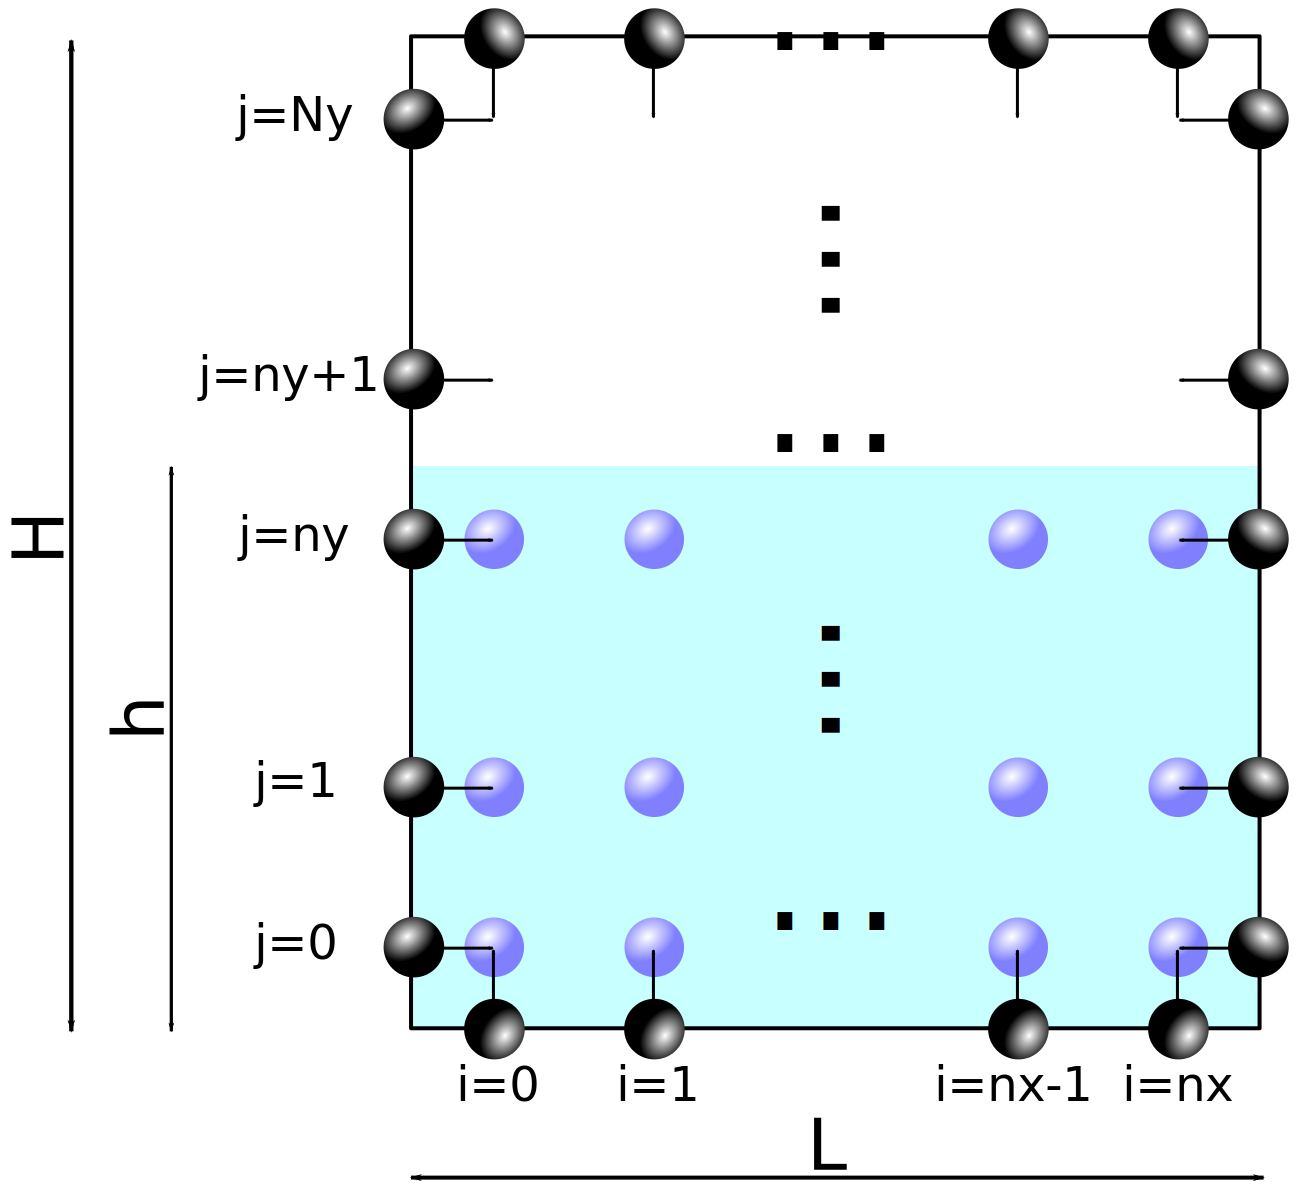
\includegraphics[width=0.8\textwidth]{lateral_water_1x_deleffe/particles}
  \caption{Particles packing scheme}
  \label{fig:examples:lateral_water_1x_deleffe:particles_packing}
\end{figure}
%
\subsection{Time discretization}
\label{ss:example:lateral_water_1x_deleffe:timing}
%
In \NAME the time is discretized in order to forward integrate it using the Leap-Frog scheme
documented in section \ref{ss:aquagpusph:leapfrog}. To perform the time discretization 2 main
magnitudes must be controlled, the simulation total time, and the time step. Also we can setup
a stabilization time.\rc
%
First for all create the XML definition file ``\textbf{Time.xml}'' with the section called
``Timing''. We want to run a simulation of 5 seconds without a stabilization stage and with a
time step such that is adapted in real time to fit to the criteria described in section
\ref{ss:sph:discrete:timestep}, that in this type of cases can be really useful due to in the
sloshing instant some particles can significantly accelerate getting high velocities, but
reducing the time step we can manage the situation. To set these options we add following tags
into the ``Timing'' section:
%
\begin{verbatim}
<Option name="SimulationStop" type="Time" value="5.0" />
<Option name="TimeStep" value="Variable"/>
<Option name="Stabilization" value="0.0"/>
\end{verbatim}
%
In order to improve the Courant number a division factor can be set as described in section
\ref{sss:XML:SPH}, in our case we will set a factor of 4 adding following option to the ``SPH''
section of the definition file ``SPH.xml'':
%
\begin{verbatim}
<Option name="DivDt" value="4.0" />
\end{verbatim}
%
\subsection{Output configuration}
\label{ss:example:lateral_water_1x_deleffe:output}
%
In order to post-process the simulation we want several output files:
%
\begin{enumerate}
	\item Sensor pressure: In the main output, and will require to set some sensors in the walls.
	\item Visualization: H5Part output files will be written in order to can perform
	visualizations with Paraview.
	\item Log file: In order to get a general view of the simulation process with relevant
	incidents, notifications and errors.
	\item Energy: An energy log along the simulation will be written too.
\end{enumerate}
%
In order to create the sensor 1 shown in the figure
\ref{fig:examples:lateral_water_1x_deleffe_scheme:scheme} we will add several measuring points in
order to can cover all the real sensor area\footnote{Must be noticed that in the case that kernel
height $h$ is greater than the sensor length, adding several points will not make effect since you
don't have resolution, but you can consider adding it in order to future resolution increasing.}.
To do it create the XML definition file ``Sensors.xml'' with the following content:
%
\begin{verbatim}
<?xml version="1.0" ?>
<sphInput>
	<Sensors>
		<FPS value="10000.0" />
		<Script file="/usr/share/aquagpusph/resources/OpenCL/Sensors" />
		<Sensor x="-0.45" y="0.09300" type="Interpolated" />
		<Sensor x="-0.45" y="0.09275" type="Interpolated" />
		<Sensor x="-0.45" y="0.09250" type="Interpolated" />
		<Sensor x="-0.45" y="0.09225" type="Interpolated" />
		<Sensor x="-0.45" y="0.09200" type="Interpolated" />
		<Sensor x="-0.45" y="0.09325" type="Interpolated" />
		<Sensor x="-0.45" y="0.09350" type="Interpolated" />
		<Sensor x="-0.45" y="0.09375" type="Interpolated" />
		<Sensor x="-0.45" y="0.09400" type="Interpolated" />
	</Sensors>
</sphInput>
\end{verbatim}
%
See the section \ref{sss:XML:Sensors} for further details about the options introduced. To set the
rest of output files edit the file ``\textbf{Time.xml}'' adding following options into section
``Timing'':
%
\begin{verbatim}
<Option name="Output" format="H5Part" type="FPS" value="30" />
<Option name="LogFiles" type="FPS" value="120" />
<Option name="EnFiles" type="FPS" value="120" />
<Option name="BoundsFiles" type="No" />
\end{verbatim}
%
Take care to don't set too high frequency of the visualization file output because huge hard disk
demand can be expected.
%
\subsection{Other options}
\label{ss:example:lateral_water_1x_deleffe:settings}
%
We may set some general \NAME settings, see section \ref{sss:XML:Settings} to learn more about the
general options. To set this options simply generate a file called ``Settings.xml'' with the following
content:
%
\begin{verbatim}
<?xml version="1.0" ?>
<sphInput>
	<Settings>
		<Verbose level="1" />
		<Start mode="0" />
	</Settings>
</sphInput>
\end{verbatim}
%
\subsection{Main XML definition file}
\label{ss:example:lateral_water_1x_deleffe:mainXML}
%
We have been generated following files:
%
\begin{itemize}
	\item Fluids.xml
	\item Movements.xml
	\item OpenCL.xml
	\item Sensors.xml
	\item Settings.xml
	\item SPH.xml
	\item Time.xml
	\item CreateMotions.py
	\item CreateParticles.py
	\item Particles.dat
	\item Move/6DOF.xml
	\item Move/6DOF.dat
	\item doc/lateral\_water\_1x.txt
\end{itemize}
%
The data files with the motions or the spatial discretization have been referenced into the corresponding
XML files, and the specific motion definition file ``Move/6DOF.xml'' has been referenced from the general
motions definition file ``Movements.xml'', but all the separately XML definition files must be grouped into
a general definition file that will load \NAME in order to setup the case. Create a file called
``\textbf{Main.xml}'' with the following content:
%
\begin{verbatim}
<?xml version="1.0" ?>
<sphInput>
	<Include file="Fluids.xml" />
	<Include file="Movements.xml" />
	<Include file="OpenCL.xml" />
	<Include file="Sensors.xml" />
	<Include file="Settings.xml" />
	<Include file="SPH.xml" />
	<Include file="Time.xml" />
</sphInput>
\end{verbatim}
%
This file don't contains any relevant data, only redirects \NAME to read all the other previously generated
files.
%
\subsection{Run the simulation}
\label{ss:example:lateral_water_1x_deleffe:running}
%
This case has been generated using relative paths\footnote{Relative paths provided into the configuration
files are ever relatives to the execution path, not to the XML path}, so must be executed in the root folder
where we have been generated it. Running the case is so quite easy, simply open a terminal in the folder where
you have the file ``\textbf{Main.xml}'' and execute
%
\begin{verbatim}
AQUAgpusph2D --input Main.xml --no-reassembly
\end{verbatim}
%
See section \ref{ss:running:launching} to learn more about the cases launch process and the messages that you
will receive while \NAME is running, and it's stored in the log file ``Log.html''. Depending on hardware used
the simulation can take from 2 hours to more than 10 hours, so consider reduce the resolution or the number of
neighbours in this case.
%
\subsection{Post-process the simulation}
\label{ss:example:lateral_water_1x_deleffe:postprocess}
%
\subsubsection{General}
\label{sss:example:lateral_water_1x_deleffe:postprocess:general}
%
Post-process can be divided in 2 main categories:
%
\begin{enumerate}
	\item Run time post-process
	\item Finished simulation post-process
\end{enumerate}
%
The first one has the advantage that can be performed while the simulation is running, and consist mainly on
plots of output data. The second one is mainly the visualization with the H5Part output.
%
\subsubsection{Run rime post-process}
\label{sss:example:lateral_water_1x_deleffe:postprocess:gnuplot}
%
In this case the main objective is to plot the pressure obtained on sensor 1 (see figure
\ref{fig:examples:lateral_water_1x_deleffe_scheme:scheme}), that is included in the data that can be processed
in run time. We will use intensively \textbf{gnuplot} and \textbf{awk} along this section.\rc
%
You can find more data about how is sensors file formatted in the section \ref{ss:aquagpusph:sensors}. Basically
we want to read the pressure data on each of the 9 measuring points placed around sensor 1 position, and plot
the average value along the time. With \textbf{awk}, get this pressure for each time instant written can be
performed typing in a terminal on the execution folder
%
\begin{verbatim}
awk '{p=$4+$9+$14+$19+$24+$29+$34+$39+$44;p=p/9.0; print $1,p}' Sensors.dat
\end{verbatim}
%
That loads the sensors output file ``Sensors.dat'', compute the required value for each time step, and return
2 columns with the time instants and the pressure obtained. Regarding the experimental data, pressure has been
measured in mbar, so we need to move it to Pa:
%
\begin{verbatim}
awk '{p=$2; print $1,100.0*p}' lateral_water_1x.txt
\end{verbatim}
%
So we can obtain, using \textbf{awk}, 2 files that contains the experimental and simulated pressures, so we only
need to create a \textbf{gnuplot} layout, that we can call ``\textbf{press.gnuplot}'' (place it in the root
folder), that uses internally \textbf{awk} to plot the desired data.
%
\begin{verbatim}
# Set plot options
set key
set grid
# Set x parameters
set xlabel "Time [s]"
set xtic
set xrange[0:5]
# Set left y parameters
set ylabel "Pressure [Pa]"
set ytic
set yrange[-1000:5000]
# Line styles
set style line 1 lt -1 lw 1
set style line 2 lt -1 lc rgb "red" lw 1

# Plot
plot \
"<awk '{p=$2; print $1,100.0*p}' doc/lateral_water_1x.txt" \
using 1:2 title 'Experimental' axes x1y1 with lines ls 2, \
"<awk '{p=$4+$9+$14+$19+$24+$29+$34+$39+$44;p=p/9.0; print $1,p}' Sensors.dat" \
using 1:2 title 'SPH' axes x1y1 with lines ls 1

pause 5
replot
reread
\end{verbatim}
%
The script shown above will plot the pressure data while it is available, reploting with in an interval of 5
seconds. In the figure \ref{fig:examples:lateral_water_1x_deleffe:sensors} you can see a pressure plot example
that you can expect using \textbf{gnuplot}.\rc
%
As you can see the results can be significantly improved as shown in the publication \citep{Maciaetal_PTP_2012}
where this simulation example was introduced, but is enough for our purposes. Feel free to play with the
parameters and see the effects.\rc
%
In the same way described you can plot the energy graphs.
%
\begin{figure}[h!]
  \centering
  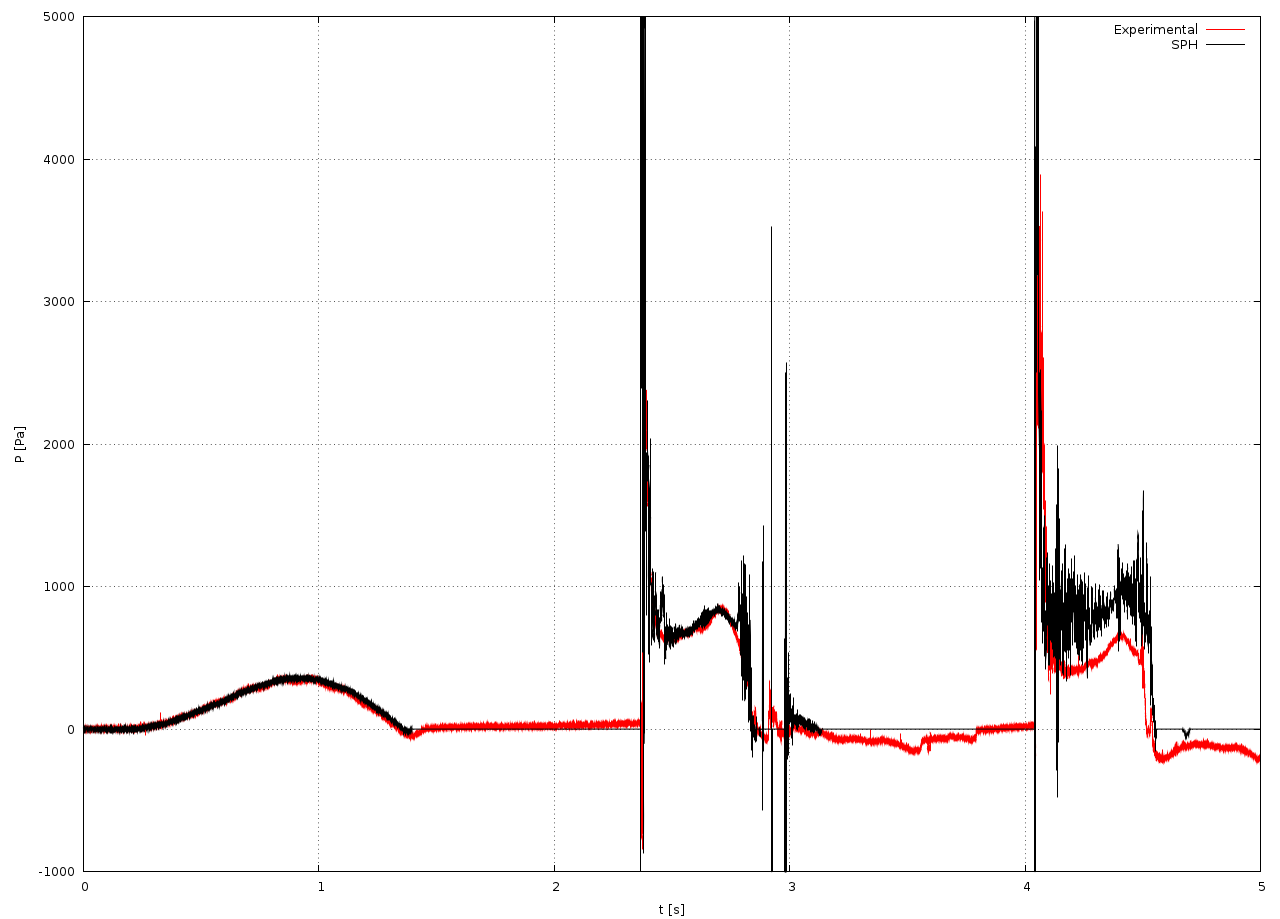
\includegraphics[width=0.7\textwidth]{lateral_water_1x_deleffe/sensors_freeslip}
  \caption{Pressure register comparison between experimental and simulation data}
  \label{fig:examples:lateral_water_1x_deleffe:sensors}
\end{figure}
%
\subsubsection{Finished simulation post-process}
\label{sss:example:lateral_water_1x_deleffe:postprocess:paraview}
%
When the simulation has finished we can work over the H5Part output file. In this section we will use
\textbf{Paraview}. Remember that your \textbf{Paraview} needs the H5Part files loader plugin to can run.\rc
%
To start working executes Paraview, and go to ``File/Open''. A new window opens in order to select a file to
open, so select the output file ``Particles0.h5part'' and accept. At this point you still not seeing nothing
on the 3D view, but a new filter has been added to the pipeline, as you can see in the figure
\ref{fig:examples:lateral_water_1x_deleffe:paraviewfilter}. Below the pipeline you can find the options of
this filter, ensure that $Xarray$, $Yarray$ and $zArray$ are right, and press \textbf{Apply}. In the figure
\ref{fig:examples:lateral_water_1x_deleffe:paraviewfilteroptions} you can see how the options must be set.\rc
%
After that something is shown in the 3D view, our first objective will be separate in 3 different instances
the walls elements, the fluid particles, and the sensors, to do it we need to apply 4 filters, one to extract
solid that has $imove < 0$ flag, another one to extract fluid that has $imove > 0$ flag, and 2 more filters
for sensors that has $imove = 0$ flag.\rc
%
Go to \textbf{Filters/Common/Clip}, and a new filter depending on our original one is added. You can change
the filter name selecting it in the pipeline browser, and pressing ``F2'', set the name ``\textbf{Solid}''.
Now set the options in the object inspector as shown in figure
\ref{fig:examples:lateral_water_1x_deleffe:paraviewsolidfilter}, and press Apply. In 3D view only solid
elements are shown now.\rc
%
Before to get fluid particles we will format solid elements style. Change to the ``Display'' tab, and modify
``Color by'' option to \textbf{Solid Color}. Change the ``point size'' to \textbf{1.00} too in the ``Style''
section. You may see something similar to the presented on figure
\ref{fig:examples:lateral_water_1x_deleffe:paraviewsolid3D}.\rc
%
Selecting the H5Part file instnace apply now another \textbf{Clip} filter, but in this case select the
``Value'' \textbf{0.5}, and uncheck ``Inside Out'', naming to this new instance ``\textbf{Fluid}''.\rc
%
The fluid can be styled selecting ``Color by'' as \textbf{press}, and pressing ``Edit Color Map'' we can edit
the color mapping behaviour. In figure \ref{fig:examples:lateral_water_1x_deleffe:paraviewcolormap} the options
selected for the color map, in order to get the visualization shown in the figure
\ref{fig:examples:lateral_water_1x_deleffe:paraviewfluid3D} is shown. You can show the legend with the options
of the ``Color Legend'' tab of the same window.\rc
%
Finally add 2 new \textbf{Clip} filters, apply the first one to the H5Part loaded instance, with the ``Value''
\textbf{-0.5}, but with ``Inside Out'' unchecked, and apply the another filter to the first one with theç
``Value'' \textbf{0.5} and ``Inside Out'' checked. You can rename both filters as ``\textbf{Sensors}''.\rc
%
Sensors must be coloured with \textbf{press} too, but in this case the ``point size'' can be increased to and
hight value, for instance \textbf{3.0}.\rc
%
Finally you can change the background color with \textbf{Edit/View Settings...}. In this window you can also
set/unset the parallel projection\footnote{Is strongly recommended use parallel projection} and the
annotations.\rc
%
Now you have your visualization formatted, and you can start animating and saving images/videos.In the figure
\ref{fig:examples:lateral_water_1x_deleffe:paraviewanimation} you can see an example of an animation performed
with ParaView.\rc
%
You can additionally save a ParaView state that when you loads it apply automatically all the purposed filters.
%
\begin{figure}[ht!]
  \centering
  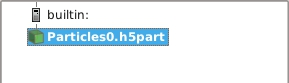
\includegraphics[width=0.3\textwidth]{lateral_water_1x_deleffe/paraviewfilter}
  \caption{Filter added to Paraview}
  \label{fig:examples:lateral_water_1x_deleffe:paraviewfilter}
\end{figure}
%
\begin{figure}[ht!]
  \centering
  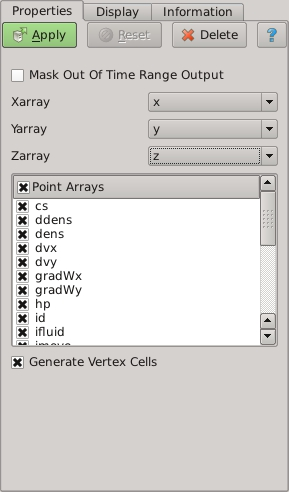
\includegraphics[width=0.3\textwidth]{lateral_water_1x_deleffe/paraviewfilteroptions}
  \caption{H5Part loaded file options}
  \label{fig:examples:lateral_water_1x_deleffe:paraviewfilteroptions}
\end{figure}
%
\begin{figure}[ht!]
  \centering
  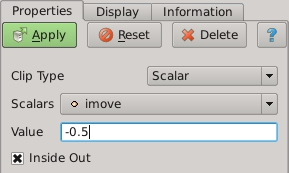
\includegraphics[width=0.3\textwidth]{lateral_water_1x_deleffe/paraviewsolidfilter}
  \caption{Solid Clip filter options}
  \label{fig:examples:lateral_water_1x_deleffe:paraviewsolidfilter}
\end{figure}
%
\begin{figure}[ht!]
  \centering
  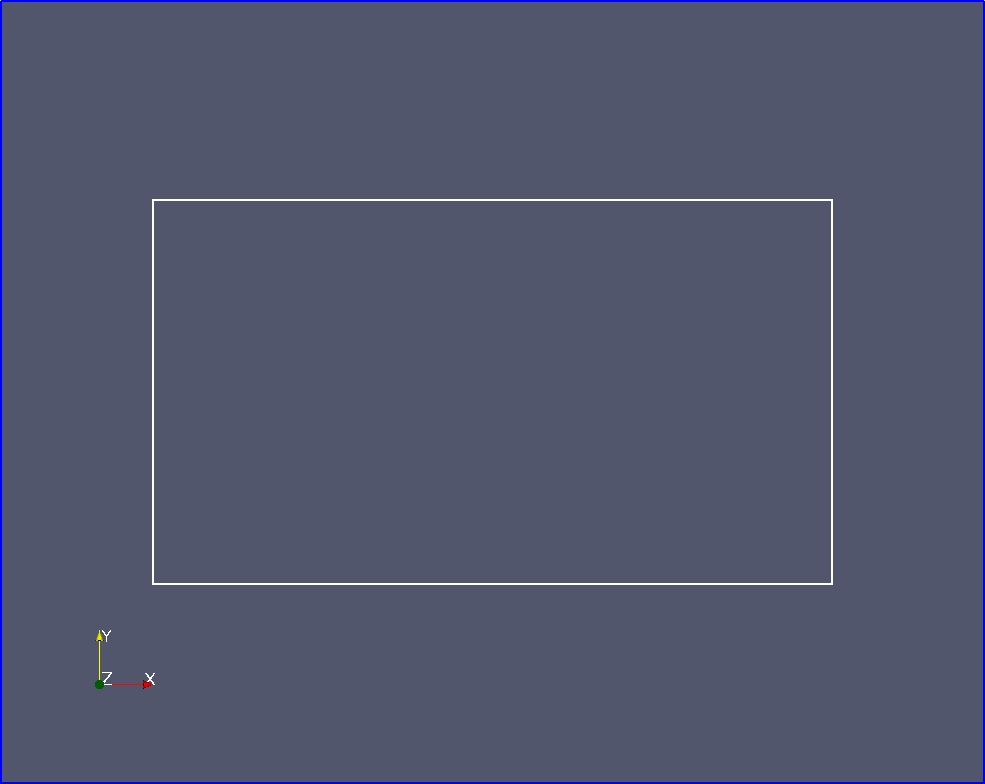
\includegraphics[width=0.5\textwidth]{lateral_water_1x_deleffe/paraviewsolid3D}
  \caption{3D view with only the solid elements}
  \label{fig:examples:lateral_water_1x_deleffe:paraviewsolid3D}
\end{figure}
%
\begin{figure}[ht!]
  \centering
  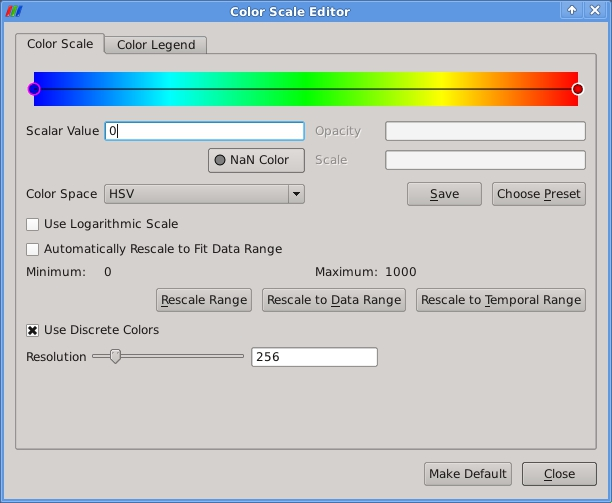
\includegraphics[width=0.4\textwidth]{lateral_water_1x_deleffe/paraviewcolormap}
  \caption{Pressure color map options}
  \label{fig:examples:lateral_water_1x_deleffe:paraviewcolormap}
\end{figure}
%
\begin{figure}[ht!]
  \centering
  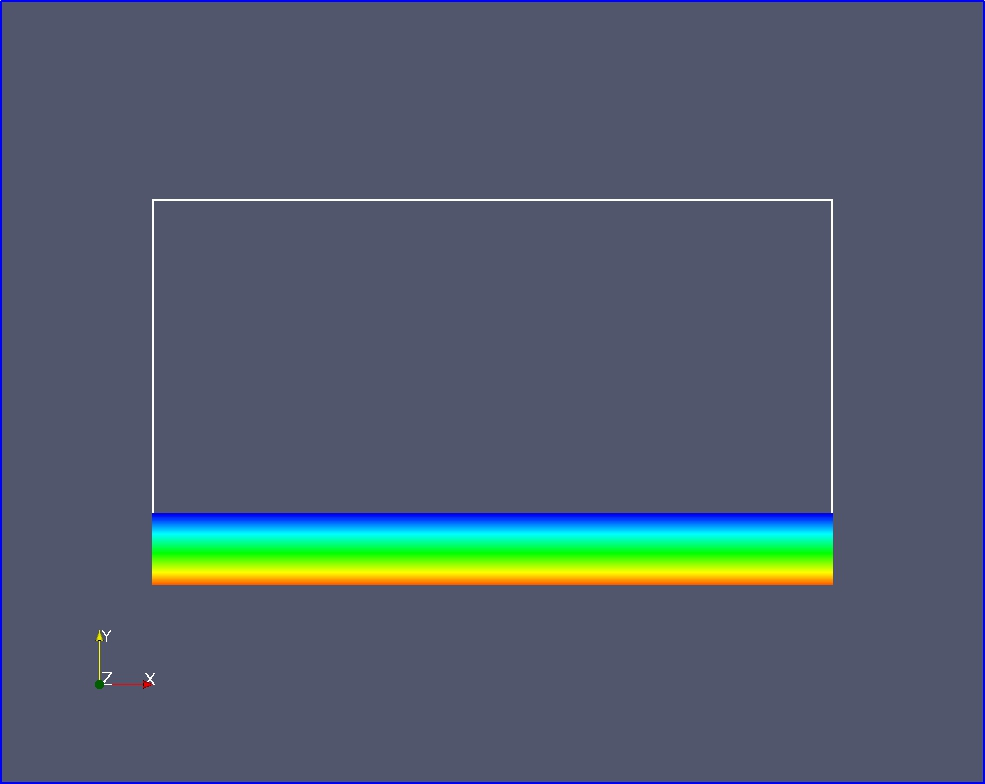
\includegraphics[width=0.5\textwidth]{lateral_water_1x_deleffe/paraviewfluid3D}
  \caption{3D view with the solid elements and the fluid particles}
  \label{fig:examples:lateral_water_1x_deleffe:paraviewfluid3D}
\end{figure}
%
\begin{figure}[ht!]
  \centering
  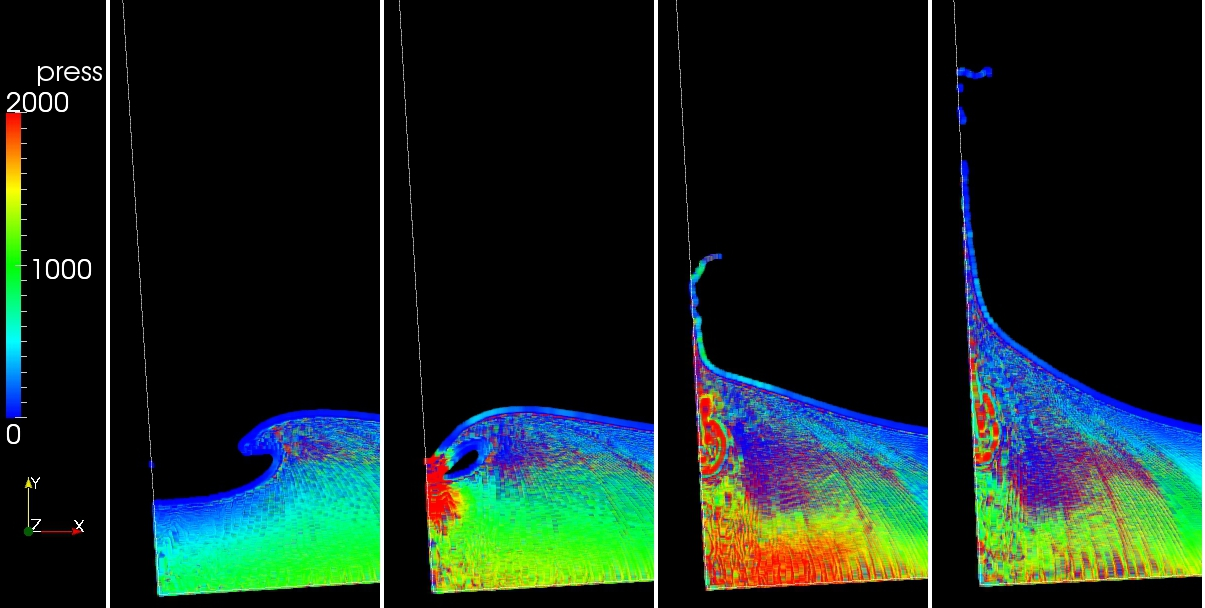
\includegraphics[width=0.7\textwidth]{lateral_water_1x_deleffe/animation_freeslip}
  \caption{Animation of the example for the first impact, frames 70-73, using free-slip boundary condition}
  \label{fig:examples:lateral_water_1x_deleffe:paraviewanimation}
\end{figure}
%
\subsection{Conclusions}
\label{ss:example:lateral_water_1x_deleffe:conclusions}
%
In this example is shown how to setup a case from scratch, that even though this is the the most complex way to
do it, is too easy to perform it. The example has been covered in detail, including the case setup, the
simulation launch, and the post-process.\rc
%
The unique tool that has been managed without text files has been Paraview, but if Paraview has been installed
with Python support, the work that we have been performed in the section
\ref{sss:example:lateral_water_1x_deleffe:postprocess:paraview} can be placed in a Python script, that is a text
file, so the entirely simulation could be easily scripted\footnote{\NAME package has internally scripted the
case with the CMake tool, that you can test it in comparing the built and installed versions, where all the paths
into the definition files and scripts are different}.\rc
%
In the results a typical Weakly compressible SPH (W-SPH) pressure noise can be noticed, but results have a good
quality.\rc
%
During the case generation we have set free-slip boundary condition along the walls because the Reynolds number
reached is so quite far from the real one (Dynamic viscosity has been artificially increased 400 times), but
we could considered that our Reynolds number is enough to set a no-slip boundary condition, with the hope that
we will receive a more stable simulation, and maybe with some better results. In the figure \ref{fig:examples:lateral_water_1x_deleffe:sensors_noslip} the pressure measured in the sensor 1 and the
simulation result using no-slip boundary condition is shown. You can compare the pressures computed using
free-slip, shown in the figure \ref{fig:examples:lateral_water_1x_deleffe:sensors}, and using no-slip,
shown in the figure \ref{fig:examples:lateral_water_1x_deleffe:sensors_noslip}, where can be noticed that the
best quality of the first one. In the figure \ref{fig:examples:lateral_water_1x_deleffe:paraviewanimation_noslip}
the same animation shown in the figure \ref{fig:examples:lateral_water_1x_deleffe:paraviewanimation} for the
free-slip is presented for the no-slip boundary condition.\rc
%
In this example we have generated all the needed files in order to perform the simulation, that are ready
installed on the system. Since we have been used relative directories to refer the files between them, we can
only execute our example from the generated location, but the installed version can be executed in whatever place
where we have permission to write. We will use this approach in the next example.\rc
%
The next example is heavy related with this one, but the boundary condition has been moved from boundary
integrals (formerly De Leffe or DeLeffe for the configuration files) to Ghost particles, that is probably the
most popular boundary condition generally used.
%
\begin{figure}[ht!]
  \centering
  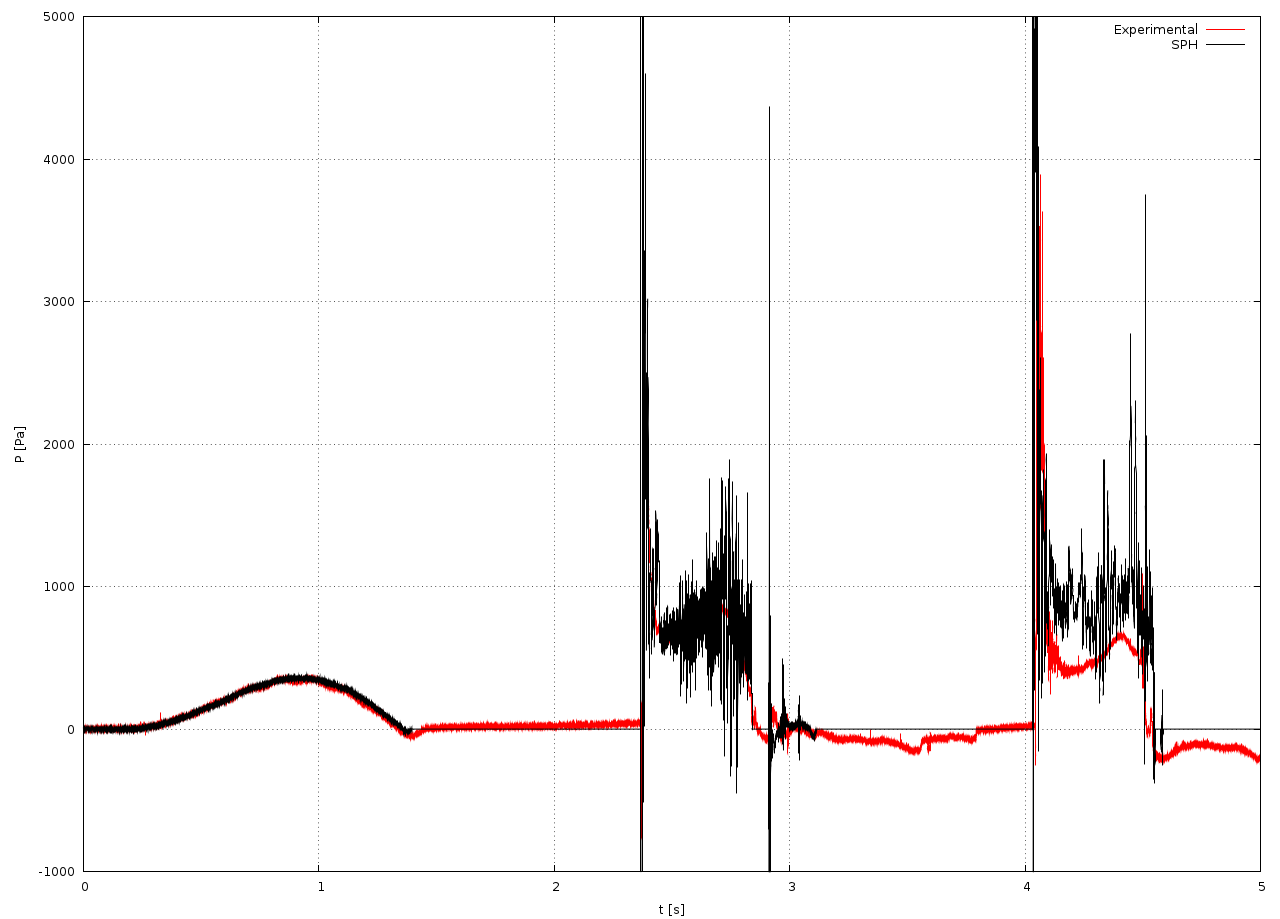
\includegraphics[width=0.7\textwidth]{lateral_water_1x_deleffe/sensors_noslip}
  \caption{Pressure register comparison between experimental and simulation data, using no-slip boundary condition}
  \label{fig:examples:lateral_water_1x_deleffe:sensors_noslip}
\end{figure}
%
\begin{figure}[ht!]
  \centering
  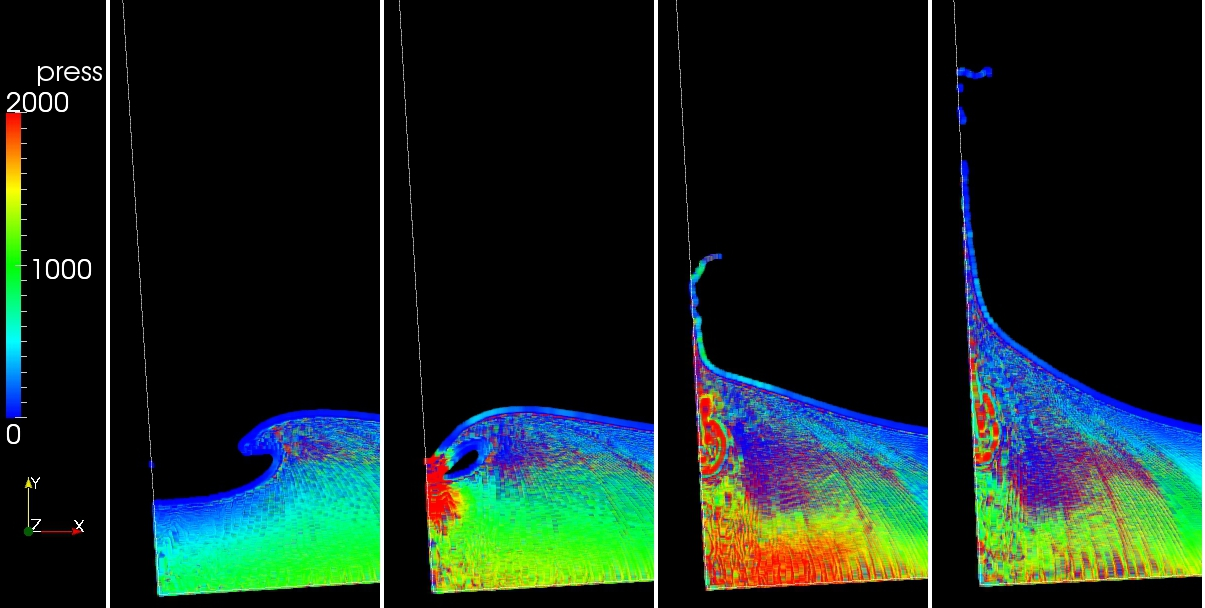
\includegraphics[width=0.7\textwidth]{lateral_water_1x_deleffe/animation_noslip}
  \caption{Animation of the example for the first impact, frames 70-73, using no-slip boundary condition}
  \label{fig:examples:lateral_water_1x_deleffe:paraviewanimation_noslip}
\end{figure}
%
%
\section{Lateral water impact 1x, with Ghost particles boundary condition}
\label{ss:example:lateral_water_1x_ghost}
%
\subsection{General}
%
This example solves the same case of the previous example described in the section
\ref{ss:example:lateral_water_1x_deleffe}, but changing the boundary condition from the De Leffe's
type to a ghost particles one, discussed on section \ref{sss:aquagpusph:boundaries:ghostparticles}.\rc
%
The objective of this example is to show how the ghost particles are used and to get a comparison on
the results obtained with each type of boundary condition.\rc
%
At the other hand, in the previous example the full process to generate a case has been documented, but
in this case we will cover only the differences with the previous example, using installed resources to run
it.\rc
%
The topics that will be covered in this example are:
%
\begin{enumerate}
	\item Configuration differences due to the boundary condition change.
	\item How to run and track a simulation installed on the system.
	\item Results comparison using either boundary integrals or ghost particles boundary conditions.
\end{enumerate}
%
In order to get a ready to run instance of this example, 2D version of \NAME package must be built, and examples
must be switched on at CMake configuration, as described in section \ref{sss:install:cmake}. You can find the
example either on the built package, at the subfolder ``examples'', and on the installed package, at\\
``\$\{CMAKE\_INSTALL\_PREFIX\}/\$\{CMAKE\_INSTALL\_DATADIR\}/examples'' (see section \ref{sss:install:cmake} to
learn more about this folder).\rc
%
Hereinafter we assume that ``\$\{CMAKE\_INSTALL\_PREFIX\}'' has been set as ``/usr'', and the example can be
found at ``/usr/share/aquagpusph/examples/LateralWater\_1x\_Ghost'' therefore.
%
\subsection{Case description}
%
You can find the case description in the section \ref{sss:example:lateral_water_1x_deleffe:caseDescription},
where the same case has been described.
%
\subsection{Settings changes required to modify the boundary condition}
%
During the section \ref{sss:example:lateral_water_1x_deleffe:BC} how to set a De Leffe's type of boundary
condition has been described. In this case this boundary condition must be deactivated, but we can use the
area elements generated to set a ``ElasticBounce'' boundary condition, described in section
\ref{sss:aquagpusph:boundaries:elasticbounce}, in order to avoid the particles trespass the walls, so the option
``Boundary'' must be moved to ``ElasticBounce'':
%
\begin{verbatim}
<Option name="Boundary" value="ElasticBounce" />
\end{verbatim}
%
Ghost particles walls are set in a different way of the other boundary conditions, where a set of special
particles are used. To set ghost particles driven walls a file called ``\textbf{GhostParticles.xml}'' is
created with the following content:
%
\begin{verbatim}
<?xml version="1.0" ?>
<sphInput>
	<GhostParticles>
		<TangentUModel value="SSM" />
		<Wall>
			<Vertex x="-0.45" y="0.0" />
			<Vertex x="0.45" y="0.0" />
		</Wall>
		<Wall>
			<Vertex x="0.45" y="0.0" />
			<Vertex x="0.45" y="0.508" />
		</Wall>
		<Wall>
			<Vertex x="0.45" y="0.508" />
			<Vertex x="-0.45" y="0.508" />
		</Wall>
		<Wall>
			<Vertex x="-0.45" y="0.508" />
			<Vertex x="-0.45" y="0.0" />
		</Wall>
		<Wall>
			<Vertex x="-0.704" y="0.254" />
			<Vertex x="0.0" y="-0.45" />
		</Wall>
		<Wall>
			<Vertex x="0.0" y="-0.45" />
			<Vertex x="0.704" y="0.254" />
		</Wall>
		<Wall>
			<Vertex x="0.704" y="0.254" />
			<Vertex x="0.0" y="0.958" />
		</Wall>
		<Wall>
			<Vertex x="0.0" y="0.958" />
			<Vertex x="-0.704" y="0.254" />
		</Wall>
	</GhostParticles>
</sphInput>
\end{verbatim}
%
In this case symmetric tangential velocity model is imposed in order to simulate free-slip boundary
condition.\rc
%
Of course this file must be referenced into ``\textbf{Main.xml}'' file too.\rc
%
Since the ``ElasticBounce'' boundary condition has been retained, the spatial discretization still being valid.
%
\subsection{Running the example installed version}
\label{ss:example:lateral_water_1x_ghost:running}
%
In this example the installed version of the example will be directly executed. To do it, create a folder
to work, for instance, a folder called ``LateralWater\_1x\_Ghost'' in your home folder, and move into:
%
\begin{verbatim}
mkdir ~/LateralWater_1x_Ghost
cd ~/LateralWater_1x_Ghost
\end{verbatim}
%
The example provides a bash script that allows to easily run the case and plot the results during the
simulation. To run the simulation type:
%
\begin{verbatim}
/usr/share/aquagpusph/examples/LateralWater_1x_Ghost/run.sh --run
\end{verbatim}
%
This command will launch \NAME with the input file set and reassembly switched off, after cleaning previous
execution results. In this case the simulation can take more time due to this boundary condition can be really
less computational efficient.\rc
%
This case will turn unstable and stop running at simulation time of 4.57208 seconds, with a time step too low to
can continue working, so when this happens cancel the job pressing `\textbf{c}' key (allowing \NAME to close
properly the case).
%
\subsection{Post-process the simulation}
\label{ss:example:lateral_water_1x_ghost:postprocess}
%
The case post-process documented along the section \ref{ss:example:lateral_water_1x_deleffe:postprocess}
still being valid in this case, but for the plotting process we can use the provided script. In another
terminal we can start the plot process executing:
%
\begin{verbatim}
/usr/share/aquagpusph/examples/LateralWater_1x_Ghost/run.sh --plot
\end{verbatim}
%
Previous command copy the motion and pressures experimental registry into the execution folder, and launch
\textit{gnuplot}. In the figure \ref{fig:examples:lateral_water_1x_ghost:sensors} the pressure register
computed using Ghost particles and the experimental one are shown. Can be noticed that with the same
resolution and number of neighbours, this boundary condition returns really worst results than the shown
in the figure \ref{fig:examples:lateral_water_1x_deleffe:sensors}, corresponding to a De Leffe's type 
free-slip boundary condition.\rc
%
In the figure \ref{fig:examples:lateral_water_1x_ghost:paraviewanimation} the first impact visualization is
shown.
%
\begin{figure}[h!]
  \centering
  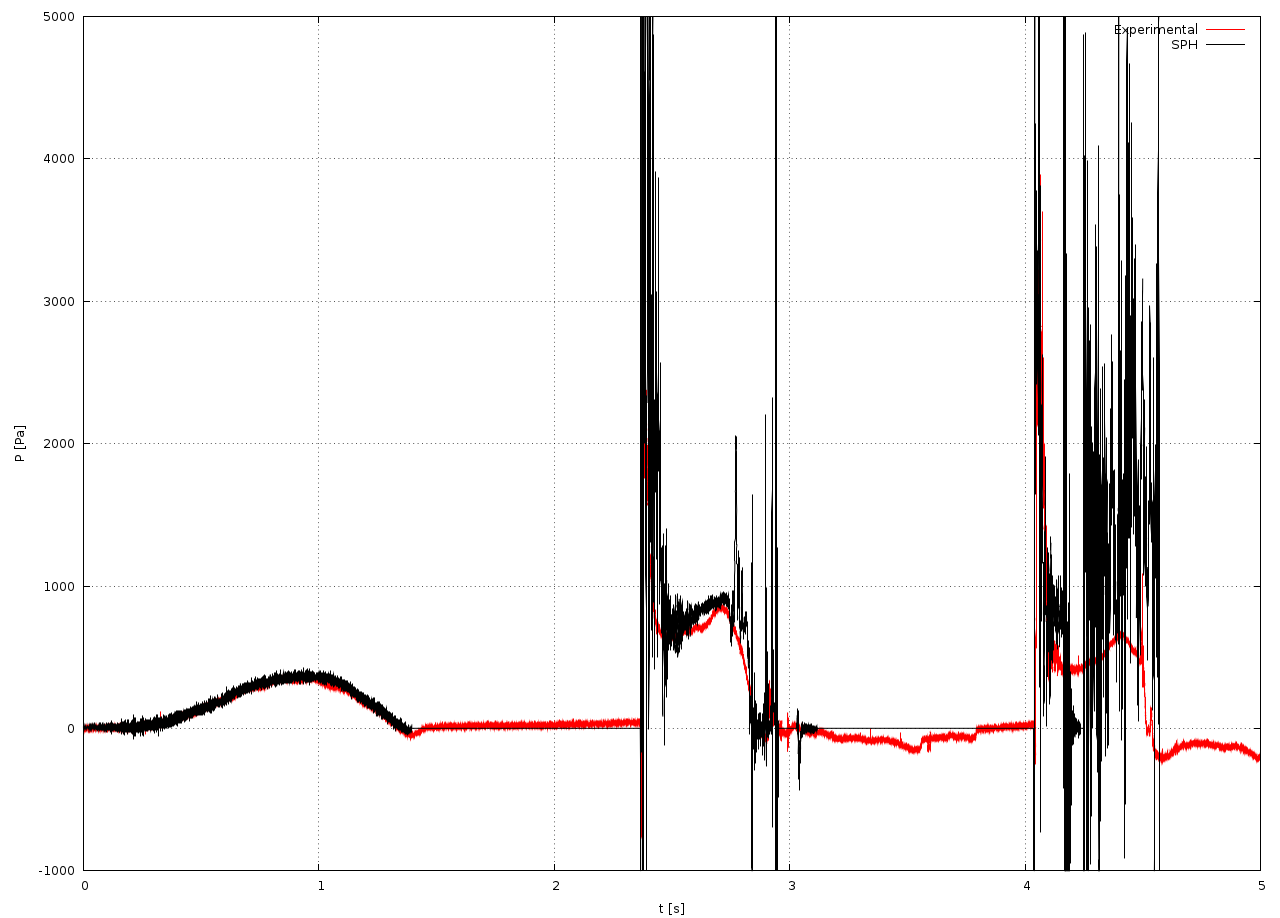
\includegraphics[width=0.7\textwidth]{lateral_water_1x_ghost/sensors_freeslip}
  \caption{Pressure register comparison between experimental and simulation data, using ghost particles and
  free-slip boundary condition (Tangent velocity SSM model)}
  \label{fig:examples:lateral_water_1x_ghost:sensors}
\end{figure}
%
\begin{figure}[ht!]
  \centering
  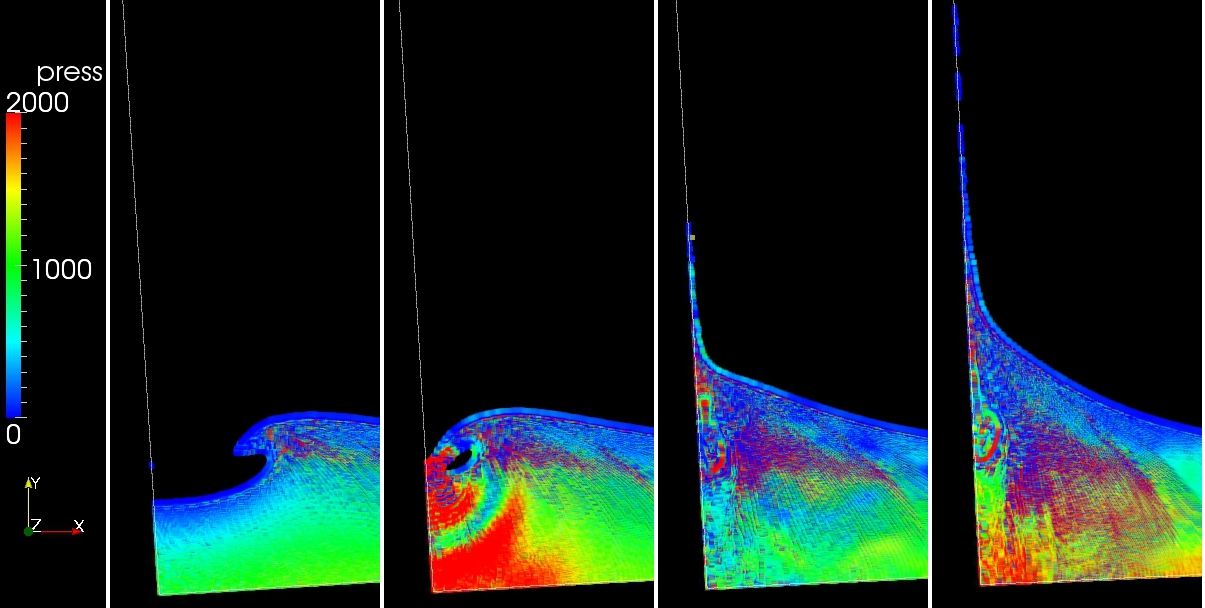
\includegraphics[width=0.7\textwidth]{lateral_water_1x_ghost/animation_freeslip}
  \caption{Animation of the example for the first impact, frames 70-73, using ghost particles and free-slip
  boundary condition}
  \label{fig:examples:lateral_water_1x_ghost:paraviewanimation}
\end{figure}
%
\subsection{Conclusions}
\label{ss:example:lateral_water_1x_deleffe:conclusions}
%
In this example two different boundary conditions has been test, the boundary integrals used in the previous
example, and the ghost particles documented along this one. Comparing figures
\ref{fig:examples:lateral_water_1x_deleffe:sensors} and \ref{fig:examples:lateral_water_1x_ghost:sensors},
corresponding to boundary integrals and ghost particles, you can see that the first one is able to reproduce
better the experimental wave impact pressure register at sensor 1.\rc
%
Also a SPH instability has been experienced in this case, causing the program crash due to a too small time step
for the used precision.\rc
%
In order to control the instability we can consider to set a no-slip boundary condition, that in the case of
ghost particles is set with the tangential velocity model, changing it from a symmetric model ``SSM'' to an
antisymmetric model ``ASM''.
%
\begin{verbatim}
<TangentUModel value="ASM" />
\end{verbatim}
%
But ``ASM'' model is inconsistent for almost general velocity fields when the Laplacian is computed, as
\ref{MaciaetalPTP} shown with polynomial velocity fields, so as $h \rightarrow 0$ the accelerations will blows up therefore, that in this case (where the resolution is fine enough) will accelerate the instability.\rc
%
In figure \ref{fig:examples:lateral_water_1x_ghost:sensors_noslip} the simulation pressure register computed until
$t \le 0.7328 s$, where the first instabilities can be appreciated much earlier than in the free-slip case.
%
\begin{figure}[h!]
  \centering
  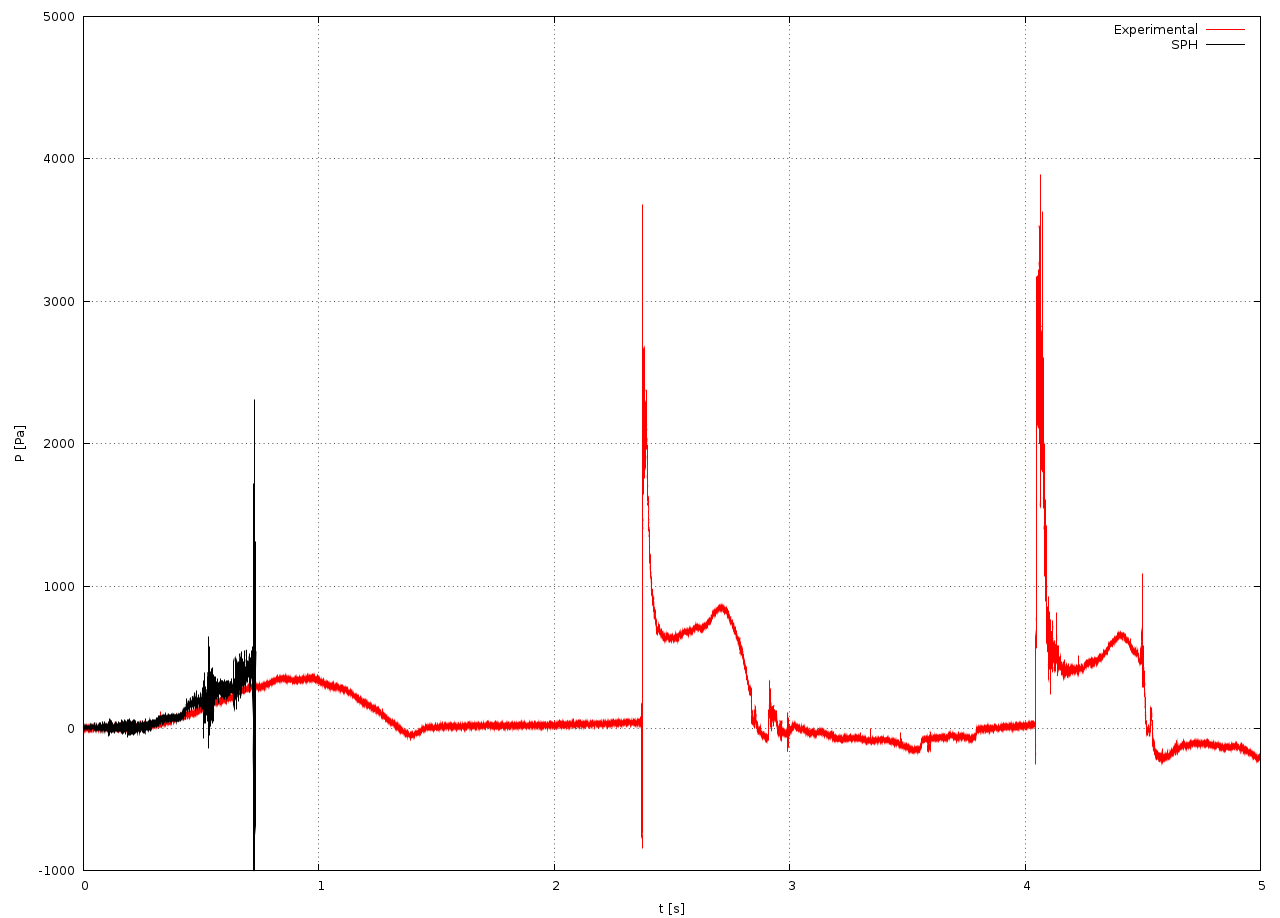
\includegraphics[width=0.7\textwidth]{lateral_water_1x_ghost/sensors_noslip}
  \caption{Pressure register comparison between experimental and simulation data, using ghost particles and
  no-slip boundary condition (Tangent velocity ASM model)}
  \label{fig:examples:lateral_water_1x_ghost:sensors_noslip}
\end{figure}
%

%


% -------------------------------
% Directory tree
% -------------------------------
\begin{appendices}
\chapter{Directory tree}
%
Following all the files provided with \NAME package, with its location, is 
shown.
%
The files autogenerated during the configuration, build and install processes 
are not shown.

\vspace{0.5cm}
\rule{\textwidth}{1pt}
\vspace{0.5cm}
\dirtree{%
.1 { 
\includegraphics[width=0.05\textwidth]{tree/Actions-document-open-folder-icon} aquagpusph }.
.2 { 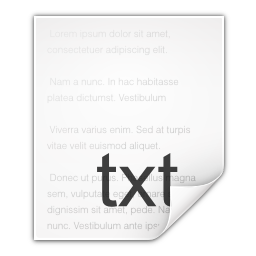
\includegraphics[width=0.05\textwidth]{tree/Mimetypes-text-plain-icon} Releases notes }.
.2 { 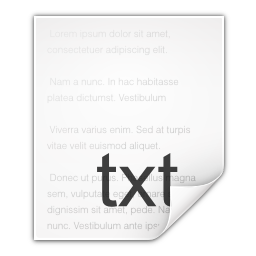
\includegraphics[width=0.05\textwidth]{tree/Mimetypes-text-plain-icon} TODO }.
.2 { 
\includegraphics[width=0.05\textwidth]{tree/Mimetypes-x-office-document-icon} LICENSE }.
.2 { 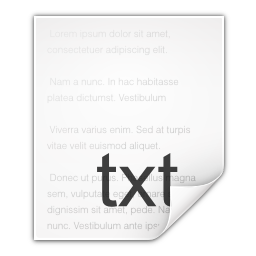
\includegraphics[width=0.05\textwidth]{tree/Mimetypes-text-plain-icon} CMakeLists.txt }.
.2 { 
\includegraphics[width=0.05\textwidth]{tree/Mimetypes-application-x-shellscript-icon} countLines.sh }.
.2 { 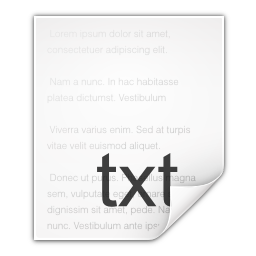
\includegraphics[width=0.05\textwidth]{tree/Mimetypes-text-plain-icon} Code styling }.
.2 { 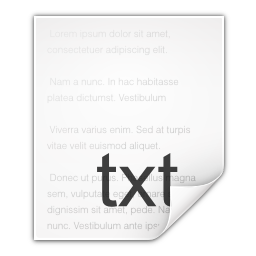
\includegraphics[width=0.05\textwidth]{tree/Mimetypes-text-plain-icon} config.h.cmake }.
.2 { 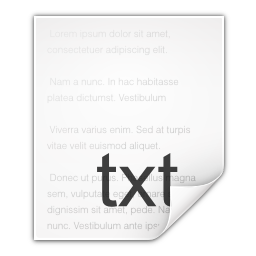
\includegraphics[width=0.05\textwidth]{tree/Mimetypes-text-plain-icon} README.md }.
.2 { 
\includegraphics[width=0.05\textwidth]{tree/Actions-document-open-folder-icon} doc }.
.3 { 
\includegraphics[width=0.05\textwidth]{tree/Mimetypes-application-pdf-icon} opencl-1-1-quick-reference-card.pdf }.
.3 { 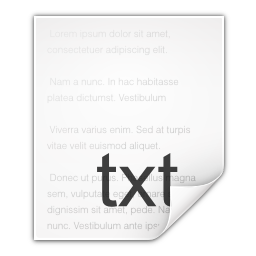
\includegraphics[width=0.05\textwidth]{tree/Mimetypes-text-plain-icon} CMakeLists.txt }.
.3 { 
\includegraphics[width=0.05\textwidth]{tree/Mimetypes-application-pdf-icon} Doxygen Quick Reference.pdf }.
.3 { 
\includegraphics[width=0.05\textwidth]{tree/Actions-document-open-folder-icon} cMake }.
.4 { 
\includegraphics[width=0.05\textwidth]{tree/Mimetypes-x-office-document-icon} Doxyfile.in }.
.3 { 
\includegraphics[width=0.05\textwidth]{tree/Actions-document-open-folder-icon} devManual }.
.4 { 
\includegraphics[width=0.05\textwidth]{tree/Mimetypes-application-pdf-icon} aquagpusph-devmanual.pdf }.
.4 { 
\includegraphics[width=0.05\textwidth]{tree/Mimetypes-x-office-document-icon} main.bbl }.
.4 { 
\includegraphics[width=0.05\textwidth]{tree/Mimetypes-text-x-bibtex-icon} directory\_tree.tex }.
.4 { 
\includegraphics[width=0.05\textwidth]{tree/Mimetypes-x-office-document-icon} main.aux }.
.4 { 
\includegraphics[width=0.05\textwidth]{tree/Mimetypes-x-office-document-icon} main.out }.
.4 { \includegraphics[width=0.05\textwidth]{tree/Mimetypes-text-x-bibtex-icon} structure.tex }.
.4 { \includegraphics[width=0.05\textwidth]{tree/Mimetypes-text-x-bibtex-icon} abstract.tex }.
.4 { \includegraphics[width=0.05\textwidth]{tree/Mimetypes-text-plain-icon} main.log }.
.4 { \includegraphics[width=0.05\textwidth]{tree/Mimetypes-application-x-shellscript-icon} buildPDF.sh }.
.4 { \includegraphics[width=0.05\textwidth]{tree/Mimetypes-x-office-document-icon} main.blg }.
.4 { \includegraphics[width=0.05\textwidth]{tree/Mimetypes-x-office-document-icon} main.toc }.
.4 { \includegraphics[width=0.05\textwidth]{tree/Mimetypes-text-x-bibtex-icon} main.tex }.
.4 { \includegraphics[width=0.05\textwidth]{tree/Mimetypes-text-x-bibtex-icon} tree\_py.tex }.
.3 { \includegraphics[width=0.05\textwidth]{tree/Actions-document-open-folder-icon} userManual }.
.4 { \includegraphics[width=0.05\textwidth]{tree/Mimetypes-text-x-bibtex-icon} running.tex }.
.4 { \includegraphics[width=0.05\textwidth]{tree/Mimetypes-text-x-bibtex-icon} lateral\_water\_1x\_ghost.tex }.
.4 { \includegraphics[width=0.05\textwidth]{tree/Mimetypes-text-x-bibtex-icon} warningMsg.tex }.
.4 { \includegraphics[width=0.05\textwidth]{tree/Mimetypes-x-office-document-icon} main.bbl }.
.4 { \includegraphics[width=0.05\textwidth]{tree/Mimetypes-text-x-bibtex-icon} elasticbounce.tex }.
.4 { \includegraphics[width=0.05\textwidth]{tree/Mimetypes-text-x-bibtex-icon} errorMsg.tex }.
.4 { \includegraphics[width=0.05\textwidth]{tree/Mimetypes-text-x-bibtex-icon} directory\_tree.tex }.
.4 { \includegraphics[width=0.05\textwidth]{tree/Mimetypes-text-x-bibtex-icon} examples.tex }.
.4 { \includegraphics[width=0.05\textwidth]{tree/Mimetypes-text-x-bibtex-icon} asciiPartsInput.tex }.
.4 { \includegraphics[width=0.05\textwidth]{tree/Mimetypes-x-office-document-icon} main.aux }.
.4 { \includegraphics[width=0.05\textwidth]{tree/Mimetypes-text-x-bibtex-icon} motionTypes.tex }.
.4 { \includegraphics[width=0.05\textwidth]{tree/Mimetypes-text-x-bibtex-icon} paraview.tex }.
.4 { \includegraphics[width=0.05\textwidth]{tree/Mimetypes-text-plain-icon} texput.log }.
.4 { \includegraphics[width=0.05\textwidth]{tree/Mimetypes-text-x-bibtex-icon} sensors.tex }.
.4 { \includegraphics[width=0.05\textwidth]{tree/Mimetypes-text-x-bibtex-icon} DeLeffe.tex }.
.4 { \includegraphics[width=0.05\textwidth]{tree/Mimetypes-text-x-bibtex-icon} infoMsg.tex }.
.4 { \includegraphics[width=0.05\textwidth]{tree/Mimetypes-text-x-bibtex-icon} ghostparticles.tex }.
.4 { \includegraphics[width=0.05\textwidth]{tree/Mimetypes-x-office-document-icon} main.out }.
.4 { \includegraphics[width=0.05\textwidth]{tree/Mimetypes-text-x-bibtex-icon} partsInput.tex }.
.4 { \includegraphics[width=0.05\textwidth]{tree/Mimetypes-text-x-bibtex-icon} aquagpusph.tex }.
.4 { \includegraphics[width=0.05\textwidth]{tree/Mimetypes-text-x-bibtex-icon} abstract.tex }.
.4 { \includegraphics[width=0.05\textwidth]{tree/Mimetypes-text-plain-icon} main.log }.
.4 { \includegraphics[width=0.05\textwidth]{tree/Mimetypes-text-x-bibtex-icon} xmlPartsInput.tex }.
.4 { \includegraphics[width=0.05\textwidth]{tree/Mimetypes-text-x-bibtex-icon} lateral\_water\_1x\_deleffe.tex }.
.4 { \includegraphics[width=0.05\textwidth]{tree/Mimetypes-application-x-shellscript-icon} buildPDF.sh }.
.4 { \includegraphics[width=0.05\textwidth]{tree/Mimetypes-x-office-document-icon} bib.bib }.
.4 { \includegraphics[width=0.05\textwidth]{tree/Mimetypes-application-pdf-icon} aquagpusph-usermanual.pdf }.
.4 { \includegraphics[width=0.05\textwidth]{tree/Mimetypes-text-x-bibtex-icon} physics.tex }.
.4 { \includegraphics[width=0.05\textwidth]{tree/Mimetypes-x-office-document-icon} main.blg }.
.4 { \includegraphics[width=0.05\textwidth]{tree/Mimetypes-text-x-bibtex-icon} install.tex }.
.4 { \includegraphics[width=0.05\textwidth]{tree/Mimetypes-x-office-document-icon} main.toc }.
.4 { \includegraphics[width=0.05\textwidth]{tree/Mimetypes-text-x-bibtex-icon} fixparticles.tex }.
.4 { \includegraphics[width=0.05\textwidth]{tree/Mimetypes-text-x-bibtex-icon} outputFiles.tex }.
.4 { \includegraphics[width=0.05\textwidth]{tree/Mimetypes-text-x-bibtex-icon} main.tex }.
.4 { \includegraphics[width=0.05\textwidth]{tree/Mimetypes-text-x-bibtex-icon} gidPartsInput.tex }.
.4 { \includegraphics[width=0.05\textwidth]{tree/Mimetypes-text-x-bibtex-icon} tree\_py.tex }.
.4 { \includegraphics[width=0.05\textwidth]{tree/Mimetypes-text-x-bibtex-icon} xmlInput.tex }.
.4 { \includegraphics[width=0.05\textwidth]{tree/Mimetypes-text-x-bibtex-icon} motionControls.tex }.
.4 { \includegraphics[width=0.05\textwidth]{tree/Actions-document-open-folder-icon} images }.
.5 { \includegraphics[width=0.05\textwidth]{tree/Mimetypes-application-x-egon-icon} GhostParticlesCorner.svg }.
.5 { \includegraphics[width=0.05\textwidth]{tree/Mimetypes-application-x-egon-icon} FixedParticles.png }.
.5 { \includegraphics[width=0.05\textwidth]{tree/Mimetypes-application-x-egon-icon} DeLeffeCorner.svg }.
.5 { \includegraphics[width=0.05\textwidth]{tree/Mimetypes-application-x-egon-icon} GhostParticles.svg }.
.5 { \includegraphics[width=0.05\textwidth]{tree/Mimetypes-application-x-egon-icon} SPHInterpolation.png }.
.5 { \includegraphics[width=0.05\textwidth]{tree/Mimetypes-application-x-egon-icon} FixedParticles.svg }.
.5 { \includegraphics[width=0.05\textwidth]{tree/Mimetypes-application-x-egon-icon} ElasticBounce.svg }.
.5 { \includegraphics[width=0.05\textwidth]{tree/Mimetypes-application-x-egon-icon} GhostParticles.png }.
.5 { \includegraphics[width=0.05\textwidth]{tree/Mimetypes-application-x-egon-icon} LinkList.png }.
.5 { \includegraphics[width=0.05\textwidth]{tree/Mimetypes-application-x-egon-icon} ElasticBounce.png }.
.5 { \includegraphics[width=0.05\textwidth]{tree/Mimetypes-application-x-egon-icon} BC.png }.
.5 { \includegraphics[width=0.05\textwidth]{tree/Mimetypes-application-x-egon-icon} CoalescenceRead.png }.
.5 { \includegraphics[width=0.05\textwidth]{tree/Mimetypes-application-x-egon-icon} DeLeffe.svg }.
.5 { \includegraphics[width=0.05\textwidth]{tree/Mimetypes-application-x-egon-icon} DeLeffeCorner.png }.
.5 { \includegraphics[width=0.05\textwidth]{tree/Mimetypes-application-x-egon-icon} GhostParticlesCorner.png }.
.5 { \includegraphics[width=0.05\textwidth]{tree/Mimetypes-application-x-egon-icon} BC.svg }.
.5 { \includegraphics[width=0.05\textwidth]{tree/Mimetypes-application-x-egon-icon} SPHInterpolation.svg }.
.5 { \includegraphics[width=0.05\textwidth]{tree/Mimetypes-application-x-egon-icon} LinkList.svg }.
.5 { \includegraphics[width=0.05\textwidth]{tree/Mimetypes-application-x-egon-icon} DeLeffe.png }.
.5 { \includegraphics[width=0.05\textwidth]{tree/Mimetypes-application-x-egon-icon} CC\_88x31.png }.
.5 { \includegraphics[width=0.05\textwidth]{tree/Mimetypes-x-office-document-icon} Diagrams.odg }.
.5 { \includegraphics[width=0.05\textwidth]{tree/Mimetypes-application-x-egon-icon} GeneralDiagram.png }.
.5 { \includegraphics[width=0.05\textwidth]{tree/Actions-document-open-folder-icon} lateral\_water\_1x\_deleffe }.
.6 { \includegraphics[width=0.05\textwidth]{tree/Mimetypes-application-x-egon-icon} paraviewfluid3D.jpg }.
.6 { \includegraphics[width=0.05\textwidth]{tree/Mimetypes-application-x-egon-icon} animation\_freeslip.jpg }.
.6 { \includegraphics[width=0.05\textwidth]{tree/Mimetypes-application-x-egon-icon} particles.png }.
.6 { \includegraphics[width=0.05\textwidth]{tree/Mimetypes-application-x-egon-icon} animation\_noslip.jpg }.
.6 { \includegraphics[width=0.05\textwidth]{tree/Mimetypes-application-pdf-icon} press.pdf }.
.6 { \includegraphics[width=0.05\textwidth]{tree/Mimetypes-application-x-egon-icon} paraviewcolormap.jpg }.
.6 { \includegraphics[width=0.05\textwidth]{tree/Mimetypes-application-x-egon-icon} paraviewfilter.jpg }.
.6 { \includegraphics[width=0.05\textwidth]{tree/Mimetypes-application-x-egon-icon} tank.png }.
.6 { \includegraphics[width=0.05\textwidth]{tree/Mimetypes-application-x-egon-icon} sensors\_noslip.png }.
.6 { \includegraphics[width=0.05\textwidth]{tree/Mimetypes-application-x-egon-icon} particles.svg }.
.6 { \includegraphics[width=0.05\textwidth]{tree/Mimetypes-application-x-egon-icon} paraviewfilteroptions.jpg }.
.6 { \includegraphics[width=0.05\textwidth]{tree/Mimetypes-application-x-egon-icon} paraviewsolid3D.jpg }.
.6 { \includegraphics[width=0.05\textwidth]{tree/Mimetypes-application-x-egon-icon} sensors\_freeslip.png }.
.6 { \includegraphics[width=0.05\textwidth]{tree/Mimetypes-application-x-egon-icon} paraviewsolidfilter.jpg }.
.6 { \includegraphics[width=0.05\textwidth]{tree/Mimetypes-x-office-document-icon} lateral\_water\_1x.gnuplot }.
.5 { \includegraphics[width=0.05\textwidth]{tree/Actions-document-open-folder-icon} wendland }.
.6 { \includegraphics[width=0.05\textwidth]{tree/Mimetypes-application-pdf-icon} wendland2D.pdf }.
.6 { \includegraphics[width=0.05\textwidth]{tree/Mimetypes-text-x-python-icon} wendland2D.py }.
.5 { \includegraphics[width=0.05\textwidth]{tree/Actions-document-open-folder-icon} tree }.
.6 { \includegraphics[width=0.05\textwidth]{tree/Mimetypes-application-x-egon-icon} Mimetypes-application-x-shellscript-icon.png }.
.6 { \includegraphics[width=0.05\textwidth]{tree/Mimetypes-application-x-egon-icon} Mimetypes-text-x-bibtex-icon.png }.
.6 { \includegraphics[width=0.05\textwidth]{tree/Mimetypes-application-x-egon-icon} Mimetypes-application-vnd-oasis-opendocument-spreadsheet-icon.png }.
.6 { \includegraphics[width=0.05\textwidth]{tree/Mimetypes-application-x-egon-icon} Mimetypes-application-xml-icon.png }.
.6 { \includegraphics[width=0.05\textwidth]{tree/Mimetypes-application-x-egon-icon} Mimetypes-application-x-egon-icon.png }.
.6 { \includegraphics[width=0.05\textwidth]{tree/Mimetypes-application-x-egon-icon} Mimetypes-application-x-archive-icon.png }.
.6 { \includegraphics[width=0.05\textwidth]{tree/Mimetypes-application-x-egon-icon} Actions-edit-select-all-icon.png }.
.6 { \includegraphics[width=0.05\textwidth]{tree/Mimetypes-application-x-egon-icon} Mimetypes-application-rtf-icon.png }.
.6 { \includegraphics[width=0.05\textwidth]{tree/Mimetypes-application-x-egon-icon} Mimetypes-text-x-c-plus-plus-src-icon.png }.
.6 { \includegraphics[width=0.05\textwidth]{tree/Mimetypes-text-x-python-icon} tree.py }.
.6 { \includegraphics[width=0.05\textwidth]{tree/Mimetypes-application-x-egon-icon} Mimetypes-text-plain-icon.png }.
.6 { \includegraphics[width=0.05\textwidth]{tree/Mimetypes-application-x-egon-icon} Mimetypes-text-x-csrc-icon.png }.
.6 { \includegraphics[width=0.05\textwidth]{tree/Mimetypes-application-x-egon-icon} Mimetypes-text-x-python-icon.png }.
.6 { \includegraphics[width=0.05\textwidth]{tree/Mimetypes-application-x-egon-icon} Mimetypes-application-x-applix-word-icon.png }.
.6 { \includegraphics[width=0.05\textwidth]{tree/Mimetypes-application-x-egon-icon} Mimetypes-application-x-desktop-icon.png }.
.6 { \includegraphics[width=0.05\textwidth]{tree/Mimetypes-application-x-egon-icon} Mimetypes-x-office-document-icon.png }.
.6 { \includegraphics[width=0.05\textwidth]{tree/Mimetypes-application-x-egon-icon} Mimetypes-application-vnd-oasis-opendocument-graphics-icon.png }.
.6 { \includegraphics[width=0.05\textwidth]{tree/Mimetypes-application-x-egon-icon} Mimetypes-application-vnd-stardivision-draw-icon.png }.
.6 { \includegraphics[width=0.05\textwidth]{tree/Mimetypes-application-x-egon-icon} Mimetypes-application-pdf-icon.png }.
.6 { \includegraphics[width=0.05\textwidth]{tree/Mimetypes-application-x-egon-icon} Mimetypes-application-octet-stream-icon.png }.
.6 { \includegraphics[width=0.05\textwidth]{tree/Mimetypes-application-x-egon-icon} Mimetypes-text-x-chdr-icon.png }.
.6 { \includegraphics[width=0.05\textwidth]{tree/Mimetypes-application-x-egon-icon} Actions-document-open-folder-icon.png }.
.5 { \includegraphics[width=0.05\textwidth]{tree/Actions-document-open-folder-icon} lateral\_water\_1x\_ghost }.
.6 { \includegraphics[width=0.05\textwidth]{tree/Mimetypes-application-x-egon-icon} animation\_freeslip.jpg }.
.6 { \includegraphics[width=0.05\textwidth]{tree/Mimetypes-application-x-egon-icon} sensors\_noslip.png }.
.6 { \includegraphics[width=0.05\textwidth]{tree/Mimetypes-application-x-egon-icon} sensors\_freeslip.png }.
.2 { \includegraphics[width=0.05\textwidth]{tree/Actions-document-open-folder-icon} tools }.
.3 { \includegraphics[width=0.05\textwidth]{tree/Mimetypes-text-x-python-icon} setup.py }.
.3 { \includegraphics[width=0.05\textwidth]{tree/Mimetypes-text-plain-icon} CMakeLists.txt }.
.3 { \includegraphics[width=0.05\textwidth]{tree/Actions-document-open-folder-icon} aquagpusph\_postprocessing }.
.4 { \includegraphics[width=0.05\textwidth]{tree/Mimetypes-x-office-document-icon} vtk-freesurface }.
.4 { \includegraphics[width=0.05\textwidth]{tree/Mimetypes-x-office-document-icon} pvd-locale }.
.3 { \includegraphics[width=0.05\textwidth]{tree/Actions-document-open-folder-icon} aquagpusph\_preprocessing }.
.4 { \includegraphics[width=0.05\textwidth]{tree/Mimetypes-x-office-document-icon} AQUAgpusph-loadGiD }.
.4 { \includegraphics[width=0.05\textwidth]{tree/Mimetypes-x-office-document-icon} AQUAgpusph-loadAbaqus }.
.4 { \includegraphics[width=0.05\textwidth]{tree/Mimetypes-text-x-python-icon} \_\_init\_\_.py }.
.4 { \includegraphics[width=0.05\textwidth]{tree/Actions-document-open-folder-icon} generator }.
.5 { \includegraphics[width=0.05\textwidth]{tree/Mimetypes-text-x-python-icon} fluid.py }.
.5 { \includegraphics[width=0.05\textwidth]{tree/Mimetypes-text-x-python-icon} vec.py }.
.5 { \includegraphics[width=0.05\textwidth]{tree/Mimetypes-text-x-python-icon} solid.py }.
.5 { \includegraphics[width=0.05\textwidth]{tree/Mimetypes-text-x-python-icon} \_\_init\_\_.py }.
.4 { \includegraphics[width=0.05\textwidth]{tree/Actions-document-open-folder-icon} mesh\_loader }.
.5 { \includegraphics[width=0.05\textwidth]{tree/Mimetypes-text-x-python-icon} Abaqus.py }.
.5 { \includegraphics[width=0.05\textwidth]{tree/Mimetypes-text-x-python-icon} GiD.py }.
.5 { \includegraphics[width=0.05\textwidth]{tree/Mimetypes-text-x-python-icon} \_\_init\_\_.py }.
.2 { \includegraphics[width=0.05\textwidth]{tree/Actions-document-open-folder-icon} examples }.
.3 { \includegraphics[width=0.05\textwidth]{tree/Mimetypes-text-plain-icon} CMakeLists.txt }.
.3 { \includegraphics[width=0.05\textwidth]{tree/Actions-document-open-folder-icon} LateralWater\_1x\_Ghost }.
.4 { \includegraphics[width=0.05\textwidth]{tree/Mimetypes-text-x-python-icon} Create.py }.
.4 { \includegraphics[width=0.05\textwidth]{tree/Actions-document-open-folder-icon} doc }.
.5 { \includegraphics[width=0.05\textwidth]{tree/Mimetypes-text-x-python-icon} plot.py }.
.5 { \includegraphics[width=0.05\textwidth]{tree/Mimetypes-application-pdf-icon} SOUTOIGLESIAS\_BOTIA\_SPHERIC\_TESTCASE\_10.pdf }.
.5 { \includegraphics[width=0.05\textwidth]{tree/Mimetypes-text-plain-icon} lateral\_water\_1x.txt }.
.4 { \includegraphics[width=0.05\textwidth]{tree/Actions-document-open-folder-icon} Move }.
.5 { \includegraphics[width=0.05\textwidth]{tree/Mimetypes-x-office-document-icon} 6DOFresources.ods }.
.5 { \includegraphics[width=0.05\textwidth]{tree/Mimetypes-text-plain-icon} 6DOF.dat }.
.3 { \includegraphics[width=0.05\textwidth]{tree/Actions-document-open-folder-icon} cMake }.
.4 { \includegraphics[width=0.05\textwidth]{tree/Actions-document-open-folder-icon} LateralWater\_1x\_Ghost }.
.5 { \includegraphics[width=0.05\textwidth]{tree/Mimetypes-application-xml-icon} Fluids.xml }.
.5 { \includegraphics[width=0.05\textwidth]{tree/Mimetypes-application-xml-icon} GhostParticles.xml }.
.5 { \includegraphics[width=0.05\textwidth]{tree/Mimetypes-application-xml-icon} Time.xml }.
.5 { \includegraphics[width=0.05\textwidth]{tree/Mimetypes-application-xml-icon} Sensors.xml }.
.5 { \includegraphics[width=0.05\textwidth]{tree/Mimetypes-application-x-shellscript-icon} run.sh }.
.5 { \includegraphics[width=0.05\textwidth]{tree/Mimetypes-application-xml-icon} Movements.xml }.
.5 { \includegraphics[width=0.05\textwidth]{tree/Mimetypes-application-xml-icon} Settings.xml }.
.5 { \includegraphics[width=0.05\textwidth]{tree/Mimetypes-application-xml-icon} SPH.xml }.
.5 { \includegraphics[width=0.05\textwidth]{tree/Mimetypes-application-xml-icon} Main.xml }.
.5 { \includegraphics[width=0.05\textwidth]{tree/Actions-document-open-folder-icon} Move }.
.6 { \includegraphics[width=0.05\textwidth]{tree/Mimetypes-application-xml-icon} 6DOF.xml }.
.4 { \includegraphics[width=0.05\textwidth]{tree/Actions-document-open-folder-icon} LateralWater\_1x\_Fix }.
.5 { \includegraphics[width=0.05\textwidth]{tree/Mimetypes-application-xml-icon} Fluids.xml }.
.5 { \includegraphics[width=0.05\textwidth]{tree/Mimetypes-application-xml-icon} Time.xml }.
.5 { \includegraphics[width=0.05\textwidth]{tree/Mimetypes-application-xml-icon} Sensors.xml }.
.5 { \includegraphics[width=0.05\textwidth]{tree/Mimetypes-application-x-shellscript-icon} run.sh }.
.5 { \includegraphics[width=0.05\textwidth]{tree/Mimetypes-application-xml-icon} Movements.xml }.
.5 { \includegraphics[width=0.05\textwidth]{tree/Mimetypes-application-xml-icon} Settings.xml }.
.5 { \includegraphics[width=0.05\textwidth]{tree/Mimetypes-application-xml-icon} SPH.xml }.
.5 { \includegraphics[width=0.05\textwidth]{tree/Mimetypes-application-xml-icon} Main.xml }.
.5 { \includegraphics[width=0.05\textwidth]{tree/Actions-document-open-folder-icon} Move }.
.6 { \includegraphics[width=0.05\textwidth]{tree/Mimetypes-application-xml-icon} 6DOF.xml }.
.4 { \includegraphics[width=0.05\textwidth]{tree/Actions-document-open-folder-icon} perezrojas\_etal\_stab\_2012 }.
.5 { \includegraphics[width=0.05\textwidth]{tree/Mimetypes-application-xml-icon} Fluids.xml }.
.5 { \includegraphics[width=0.05\textwidth]{tree/Mimetypes-application-xml-icon} Time.xml }.
.5 { \includegraphics[width=0.05\textwidth]{tree/Mimetypes-application-x-shellscript-icon} run.sh }.
.5 { \includegraphics[width=0.05\textwidth]{tree/Mimetypes-application-xml-icon} Movements.xml }.
.5 { \includegraphics[width=0.05\textwidth]{tree/Mimetypes-application-xml-icon} Settings.xml }.
.5 { \includegraphics[width=0.05\textwidth]{tree/Mimetypes-application-xml-icon} SPH.xml }.
.5 { \includegraphics[width=0.05\textwidth]{tree/Mimetypes-application-xml-icon} Main.xml }.
.5 { \includegraphics[width=0.05\textwidth]{tree/Actions-document-open-folder-icon} Move }.
.6 { \includegraphics[width=0.05\textwidth]{tree/Mimetypes-text-x-python-icon} move.py }.
.6 { \includegraphics[width=0.05\textwidth]{tree/Mimetypes-application-xml-icon} 6DOF.xml }.
.4 { \includegraphics[width=0.05\textwidth]{tree/Actions-document-open-folder-icon} lobovsky\_etal\_jfs\_2014 }.
.5 { \includegraphics[width=0.05\textwidth]{tree/Mimetypes-application-xml-icon} Fluids.xml }.
.5 { \includegraphics[width=0.05\textwidth]{tree/Mimetypes-application-xml-icon} Time.xml }.
.5 { \includegraphics[width=0.05\textwidth]{tree/Mimetypes-application-xml-icon} Sensors.xml }.
.5 { \includegraphics[width=0.05\textwidth]{tree/Mimetypes-application-x-shellscript-icon} run.sh }.
.5 { \includegraphics[width=0.05\textwidth]{tree/Mimetypes-application-xml-icon} Settings.xml }.
.5 { \includegraphics[width=0.05\textwidth]{tree/Mimetypes-application-xml-icon} SPH.xml }.
.5 { \includegraphics[width=0.05\textwidth]{tree/Mimetypes-application-xml-icon} Main.xml }.
.4 { \includegraphics[width=0.05\textwidth]{tree/Actions-document-open-folder-icon} LateralWater\_1x\_DeLeffe }.
.5 { \includegraphics[width=0.05\textwidth]{tree/Mimetypes-application-xml-icon} Fluids.xml }.
.5 { \includegraphics[width=0.05\textwidth]{tree/Mimetypes-application-xml-icon} Time.xml }.
.5 { \includegraphics[width=0.05\textwidth]{tree/Mimetypes-application-xml-icon} Sensors.xml }.
.5 { \includegraphics[width=0.05\textwidth]{tree/Mimetypes-application-x-shellscript-icon} run.sh }.
.5 { \includegraphics[width=0.05\textwidth]{tree/Mimetypes-application-xml-icon} Movements.xml }.
.5 { \includegraphics[width=0.05\textwidth]{tree/Mimetypes-application-xml-icon} Settings.xml }.
.5 { \includegraphics[width=0.05\textwidth]{tree/Mimetypes-application-xml-icon} SPH.xml }.
.5 { \includegraphics[width=0.05\textwidth]{tree/Mimetypes-application-xml-icon} Main.xml }.
.5 { \includegraphics[width=0.05\textwidth]{tree/Actions-document-open-folder-icon} Move }.
.6 { \includegraphics[width=0.05\textwidth]{tree/Mimetypes-application-xml-icon} 6DOF.xml }.
.3 { \includegraphics[width=0.05\textwidth]{tree/Actions-document-open-folder-icon} LateralWater\_1x\_Fix }.
.4 { \includegraphics[width=0.05\textwidth]{tree/Mimetypes-text-x-python-icon} Create.py }.
.4 { \includegraphics[width=0.05\textwidth]{tree/Actions-document-open-folder-icon} doc }.
.5 { \includegraphics[width=0.05\textwidth]{tree/Mimetypes-text-x-python-icon} plot.py }.
.5 { \includegraphics[width=0.05\textwidth]{tree/Mimetypes-application-pdf-icon} SOUTOIGLESIAS\_BOTIA\_SPHERIC\_TESTCASE\_10.pdf }.
.5 { \includegraphics[width=0.05\textwidth]{tree/Mimetypes-text-plain-icon} lateral\_water\_1x.txt }.
.4 { \includegraphics[width=0.05\textwidth]{tree/Actions-document-open-folder-icon} Move }.
.5 { \includegraphics[width=0.05\textwidth]{tree/Mimetypes-x-office-document-icon} 6DOFresources.ods }.
.5 { \includegraphics[width=0.05\textwidth]{tree/Mimetypes-text-plain-icon} 6DOF.dat }.
.3 { \includegraphics[width=0.05\textwidth]{tree/Actions-document-open-folder-icon} perezrojas\_etal\_stab\_2012 }.
.4 { \includegraphics[width=0.05\textwidth]{tree/Mimetypes-text-x-python-icon} Create.py }.
.4 { \includegraphics[width=0.05\textwidth]{tree/Actions-document-open-folder-icon} doc }.
.5 { \includegraphics[width=0.05\textwidth]{tree/Mimetypes-text-x-python-icon} plot.py }.
.5 { \includegraphics[width=0.05\textwidth]{tree/Mimetypes-application-pdf-icon} SOUTOIGLESIAS\_BOTIA\_SPHERIC\_TESTCASE9\_TLD.pdf }.
.4 { \includegraphics[width=0.05\textwidth]{tree/Actions-document-open-folder-icon} Move }.
.5 { \includegraphics[width=0.05\textwidth]{tree/Mimetypes-text-plain-icon} T\_1-94\_A100mm\_water.dat }.
.3 { \includegraphics[width=0.05\textwidth]{tree/Actions-document-open-folder-icon} lobovsky\_etal\_jfs\_2014 }.
.4 { \includegraphics[width=0.05\textwidth]{tree/Mimetypes-text-x-python-icon} Create.py }.
.4 { \includegraphics[width=0.05\textwidth]{tree/Actions-document-open-folder-icon} doc }.
.5 { \includegraphics[width=0.05\textwidth]{tree/Mimetypes-text-plain-icon} Fig30\_filtered\_5.dat }.
.5 { \includegraphics[width=0.05\textwidth]{tree/Mimetypes-text-plain-icon} Fig20\_filtered\_2.dat }.
.5 { \includegraphics[width=0.05\textwidth]{tree/Mimetypes-text-plain-icon} Fig12\_02\_ETSIN\_Front\_Hu\_Koshizuka\_3.dat }.
.5 { \includegraphics[width=0.05\textwidth]{tree/Mimetypes-text-plain-icon} Fig29\_filtered\_3.dat }.
.5 { \includegraphics[width=0.05\textwidth]{tree/Mimetypes-text-plain-icon} Fig31\_filtered\_1.dat }.
.5 { \includegraphics[width=0.05\textwidth]{tree/Mimetypes-text-plain-icon} Fig12\_01\_ETSIN\_Front\_Dressler\_Martin\_4.dat }.
.5 { \includegraphics[width=0.05\textwidth]{tree/Mimetypes-text-x-python-icon} sensor3.py }.
.5 { \includegraphics[width=0.05\textwidth]{tree/Mimetypes-text-plain-icon} Fig12\_01\_ETSIN\_Front\_Dressler\_Martin\_7.dat }.
.5 { \includegraphics[width=0.05\textwidth]{tree/Mimetypes-text-plain-icon} Fig12\_01\_ETSIN\_Front\_Dressler\_Martin\_6.dat }.
.5 { \includegraphics[width=0.05\textwidth]{tree/Mimetypes-text-plain-icon} Fig30\_filtered\_2.dat }.
.5 { \includegraphics[width=0.05\textwidth]{tree/Mimetypes-text-plain-icon} Fig12\_01\_ETSIN\_Front\_Dressler\_Martin\_3.dat }.
.5 { \includegraphics[width=0.05\textwidth]{tree/Mimetypes-text-plain-icon} Fig29\_filtered\_2.dat }.
.5 { \includegraphics[width=0.05\textwidth]{tree/Mimetypes-text-plain-icon} Fig31\_filtered\_4.dat }.
.5 { \includegraphics[width=0.05\textwidth]{tree/Mimetypes-text-plain-icon} Fig12\_01\_ETSIN\_Front\_Dressler\_Martin\_5.dat }.
.5 { \includegraphics[width=0.05\textwidth]{tree/Mimetypes-text-plain-icon} Fig31\_filtered\_2.dat }.
.5 { \includegraphics[width=0.05\textwidth]{tree/Mimetypes-text-plain-icon} Fig30\_filtered\_4.dat }.
.5 { \includegraphics[width=0.05\textwidth]{tree/Mimetypes-text-x-python-icon} performance.py }.
.5 { \includegraphics[width=0.05\textwidth]{tree/Mimetypes-text-plain-icon} Fig12\_01\_ETSIN\_Front\_Dressler\_Martin\_2.dat }.
.5 { \includegraphics[width=0.05\textwidth]{tree/Mimetypes-text-plain-icon} Fig29\_filtered\_4.dat }.
.5 { \includegraphics[width=0.05\textwidth]{tree/Mimetypes-text-plain-icon} Fig12\_02\_ETSIN\_Front\_Hu\_Koshizuka\_5.dat }.
.5 { \includegraphics[width=0.05\textwidth]{tree/Mimetypes-text-x-python-icon} sensor2.py }.
.5 { \includegraphics[width=0.05\textwidth]{tree/Mimetypes-text-x-python-icon} sensor1.py }.
.5 { \includegraphics[width=0.05\textwidth]{tree/Mimetypes-text-x-python-icon} sensor4.py }.
.5 { \includegraphics[width=0.05\textwidth]{tree/Mimetypes-text-plain-icon} Fig30\_filtered\_1.dat }.
.5 { \includegraphics[width=0.05\textwidth]{tree/Mimetypes-text-plain-icon} Fig29\_filtered\_1.dat }.
.5 { \includegraphics[width=0.05\textwidth]{tree/Mimetypes-text-plain-icon} Fig12\_02\_ETSIN\_Front\_Hu\_Koshizuka\_4.dat }.
.5 { \includegraphics[width=0.05\textwidth]{tree/Mimetypes-text-x-python-icon} sensors.py }.
.5 { \includegraphics[width=0.05\textwidth]{tree/Mimetypes-text-plain-icon} Fig20\_filtered\_3.dat }.
.5 { \includegraphics[width=0.05\textwidth]{tree/Mimetypes-text-plain-icon} Fig30\_filtered\_3.dat }.
.5 { \includegraphics[width=0.05\textwidth]{tree/Mimetypes-text-plain-icon} Fig20\_filtered\_1.dat }.
.5 { \includegraphics[width=0.05\textwidth]{tree/Mimetypes-text-plain-icon} Fig31\_filtered\_3.dat }.
.3 { \includegraphics[width=0.05\textwidth]{tree/Actions-document-open-folder-icon} LateralWater\_1x\_DeLeffe }.
.4 { \includegraphics[width=0.05\textwidth]{tree/Mimetypes-text-x-python-icon} Create.py }.
.4 { \includegraphics[width=0.05\textwidth]{tree/Actions-document-open-folder-icon} doc }.
.5 { \includegraphics[width=0.05\textwidth]{tree/Mimetypes-text-x-python-icon} plot.py }.
.5 { \includegraphics[width=0.05\textwidth]{tree/Mimetypes-application-pdf-icon} SOUTOIGLESIAS\_BOTIA\_SPHERIC\_TESTCASE\_10.pdf }.
.5 { \includegraphics[width=0.05\textwidth]{tree/Mimetypes-text-plain-icon} lateral\_water\_1x.txt }.
.4 { \includegraphics[width=0.05\textwidth]{tree/Actions-document-open-folder-icon} Move }.
.5 { \includegraphics[width=0.05\textwidth]{tree/Mimetypes-x-office-document-icon} 6DOFresources.ods }.
.5 { \includegraphics[width=0.05\textwidth]{tree/Mimetypes-text-plain-icon} 6DOF.dat }.
.2 { \includegraphics[width=0.05\textwidth]{tree/Actions-document-open-folder-icon} cMake }.
.3 { \includegraphics[width=0.05\textwidth]{tree/Mimetypes-text-plain-icon} FindOpenCL.cmake }.
.3 { \includegraphics[width=0.05\textwidth]{tree/Mimetypes-text-plain-icon} Findhdf5.cmake }.
.3 { \includegraphics[width=0.05\textwidth]{tree/Mimetypes-text-plain-icon} FindCurses.cmake }.
.3 { \includegraphics[width=0.05\textwidth]{tree/Mimetypes-text-plain-icon} FindXerces.cmake }.
.3 { \includegraphics[width=0.05\textwidth]{tree/Mimetypes-text-plain-icon} ConfigureChecks.cmake }.
.3 { \includegraphics[width=0.05\textwidth]{tree/Mimetypes-text-plain-icon} FindH5Part.cmake }.
.3 { \includegraphics[width=0.05\textwidth]{tree/Mimetypes-text-plain-icon} FindEigen3.cmake }.
.3 { \includegraphics[width=0.05\textwidth]{tree/Mimetypes-text-plain-icon} Findmatheval.cmake }.
.2 { \includegraphics[width=0.05\textwidth]{tree/Actions-document-open-folder-icon} include }.
.3 { \includegraphics[width=0.05\textwidth]{tree/Mimetypes-text-plain-icon} CMakeLists.txt }.
.3 { \includegraphics[width=0.05\textwidth]{tree/Mimetypes-text-x-chdr-icon} ArgumentsManager.h }.
.3 { \includegraphics[width=0.05\textwidth]{tree/Mimetypes-text-x-chdr-icon} sphPrerequisites.h }.
.3 { \includegraphics[width=0.05\textwidth]{tree/Mimetypes-text-x-chdr-icon} Singleton.h }.
.3 { \includegraphics[width=0.05\textwidth]{tree/Mimetypes-text-x-chdr-icon} ScreenManager.h }.
.3 { \includegraphics[width=0.05\textwidth]{tree/Mimetypes-text-x-chdr-icon} AuxiliarMethods.h }.
.3 { \includegraphics[width=0.05\textwidth]{tree/Mimetypes-text-x-chdr-icon} ProblemSetup.h }.
.3 { \includegraphics[width=0.05\textwidth]{tree/Mimetypes-text-x-chdr-icon} TimeManager.h }.
.3 { \includegraphics[width=0.05\textwidth]{tree/Mimetypes-text-x-chdr-icon} Fluid.h }.
.3 { \includegraphics[width=0.05\textwidth]{tree/Mimetypes-text-x-chdr-icon} CalcServer.h }.
.3 { \includegraphics[width=0.05\textwidth]{tree/Mimetypes-text-x-chdr-icon} FileManager.h }.
.3 { \includegraphics[width=0.05\textwidth]{tree/Actions-document-open-folder-icon} Tokenizer }.
.4 { \includegraphics[width=0.05\textwidth]{tree/Mimetypes-text-x-chdr-icon} Tokenizer.h }.
.3 { \includegraphics[width=0.05\textwidth]{tree/Actions-document-open-folder-icon} CalcServer }.
.4 { \includegraphics[width=0.05\textwidth]{tree/Mimetypes-text-x-chdr-icon} Torque.h }.
.4 { \includegraphics[width=0.05\textwidth]{tree/Mimetypes-text-x-chdr-icon} RadixSort.h }.
.4 { \includegraphics[width=0.05\textwidth]{tree/Mimetypes-text-x-chdr-icon} Domain.h }.
.4 { \includegraphics[width=0.05\textwidth]{tree/Mimetypes-text-x-chdr-icon} Sensors.h }.
.4 { \includegraphics[width=0.05\textwidth]{tree/Mimetypes-text-x-chdr-icon} Bounds.h }.
.4 { \includegraphics[width=0.05\textwidth]{tree/Mimetypes-text-x-chdr-icon} Corrector.h }.
.4 { \includegraphics[width=0.05\textwidth]{tree/Mimetypes-text-x-chdr-icon} LinkList.h }.
.4 { \includegraphics[width=0.05\textwidth]{tree/Mimetypes-text-x-chdr-icon} Permutate.h }.
.4 { \includegraphics[width=0.05\textwidth]{tree/Mimetypes-text-x-chdr-icon} Grid.h }.
.4 { \includegraphics[width=0.05\textwidth]{tree/Mimetypes-text-x-chdr-icon} TimeStep.h }.
.4 { \includegraphics[width=0.05\textwidth]{tree/Mimetypes-text-x-chdr-icon} Rates.h }.
.4 { \includegraphics[width=0.05\textwidth]{tree/Mimetypes-text-x-chdr-icon} DensityInterpolation.h }.
.4 { \includegraphics[width=0.05\textwidth]{tree/Mimetypes-text-x-chdr-icon} Energy.h }.
.4 { \includegraphics[width=0.05\textwidth]{tree/Mimetypes-text-x-chdr-icon} Reduction.h }.
.4 { \includegraphics[width=0.05\textwidth]{tree/Mimetypes-text-x-chdr-icon} Kernel.h }.
.4 { \includegraphics[width=0.05\textwidth]{tree/Mimetypes-text-x-chdr-icon} Shepard.h }.
.4 { \includegraphics[width=0.05\textwidth]{tree/Mimetypes-text-x-chdr-icon} Predictor.h }.
.4 { \includegraphics[width=0.05\textwidth]{tree/Actions-document-open-folder-icon} Movements }.
.5 { \includegraphics[width=0.05\textwidth]{tree/Mimetypes-text-x-chdr-icon} Quaternion.h }.
.5 { \includegraphics[width=0.05\textwidth]{tree/Mimetypes-text-x-chdr-icon} ScriptQuaternion.h }.
.5 { \includegraphics[width=0.05\textwidth]{tree/Mimetypes-text-x-chdr-icon} C1Quaternion.h }.
.5 { \includegraphics[width=0.05\textwidth]{tree/Mimetypes-text-x-chdr-icon} Movement.h }.
.5 { \includegraphics[width=0.05\textwidth]{tree/Mimetypes-text-x-chdr-icon} LinearInterpolation.h }.
.5 { \includegraphics[width=0.05\textwidth]{tree/Mimetypes-text-x-chdr-icon} C1Interpolation.h }.
.5 { \includegraphics[width=0.05\textwidth]{tree/Mimetypes-text-x-chdr-icon} LIQuaternion.h }.
.4 { \includegraphics[width=0.05\textwidth]{tree/Actions-document-open-folder-icon} Portal }.
.5 { \includegraphics[width=0.05\textwidth]{tree/Mimetypes-text-x-chdr-icon} Portal.h }.
.4 { \includegraphics[width=0.05\textwidth]{tree/Actions-document-open-folder-icon} Boundary }.
.5 { \includegraphics[width=0.05\textwidth]{tree/Mimetypes-text-x-chdr-icon} ElasticBounce.h }.
.5 { \includegraphics[width=0.05\textwidth]{tree/Mimetypes-text-x-chdr-icon} GhostParticles.h }.
.5 { \includegraphics[width=0.05\textwidth]{tree/Mimetypes-text-x-chdr-icon} DeLeffe.h }.
.3 { \includegraphics[width=0.05\textwidth]{tree/Actions-document-open-folder-icon} InputOutput }.
.4 { \includegraphics[width=0.05\textwidth]{tree/Mimetypes-text-x-chdr-icon} Log.h }.
.4 { \includegraphics[width=0.05\textwidth]{tree/Mimetypes-text-x-chdr-icon} ASCII.h }.
.4 { \includegraphics[width=0.05\textwidth]{tree/Mimetypes-text-x-chdr-icon} Report.h }.
.4 { \includegraphics[width=0.05\textwidth]{tree/Mimetypes-text-x-chdr-icon} InputOutput.h }.
.4 { \includegraphics[width=0.05\textwidth]{tree/Mimetypes-text-x-chdr-icon} State.h }.
.4 { \includegraphics[width=0.05\textwidth]{tree/Mimetypes-text-x-chdr-icon} Bounds.h }.
.4 { \includegraphics[width=0.05\textwidth]{tree/Mimetypes-text-x-chdr-icon} VTK.h }.
.4 { \includegraphics[width=0.05\textwidth]{tree/Mimetypes-text-x-chdr-icon} Energy.h }.
.4 { \includegraphics[width=0.05\textwidth]{tree/Mimetypes-text-x-chdr-icon} Particles.h }.
.2 { \includegraphics[width=0.05\textwidth]{tree/Actions-document-open-folder-icon} resources }.
.3 { \includegraphics[width=0.05\textwidth]{tree/Mimetypes-x-office-document-icon} OpenCLMain.xml.in }.
.3 { \includegraphics[width=0.05\textwidth]{tree/Mimetypes-text-plain-icon} CMakeLists.txt }.
.3 { \includegraphics[width=0.05\textwidth]{tree/Actions-document-open-folder-icon} OpenCL }.
.4 { \includegraphics[width=0.05\textwidth]{tree/Mimetypes-text-x-csrc-icon} LinkList.cl }.
.4 { \includegraphics[width=0.05\textwidth]{tree/Mimetypes-text-x-csrc-icon} Corrector.cl }.
.4 { \includegraphics[width=0.05\textwidth]{tree/Mimetypes-text-x-chdr-icon} RatesSensors.hcl }.
.4 { \includegraphics[width=0.05\textwidth]{tree/Mimetypes-text-x-csrc-icon} Shepard.cl }.
.4 { \includegraphics[width=0.05\textwidth]{tree/Mimetypes-text-x-csrc-icon} Rates.cl }.
.4 { \includegraphics[width=0.05\textwidth]{tree/Mimetypes-text-x-chdr-icon} RatesBounds.hcl }.
.4 { \includegraphics[width=0.05\textwidth]{tree/Mimetypes-text-x-csrc-icon} Energy.cl }.
.4 { \includegraphics[width=0.05\textwidth]{tree/Mimetypes-text-x-csrc-icon} Permutate.cl }.
.4 { \includegraphics[width=0.05\textwidth]{tree/Mimetypes-text-x-csrc-icon} DensInt.cl }.
.4 { \includegraphics[width=0.05\textwidth]{tree/Mimetypes-text-x-csrc-icon} RadixSort.cl }.
.4 { \includegraphics[width=0.05\textwidth]{tree/Mimetypes-text-x-csrc-icon} Torque.cl }.
.4 { \includegraphics[width=0.05\textwidth]{tree/Mimetypes-text-x-csrc-icon} Bounds.cl }.
.4 { \includegraphics[width=0.05\textwidth]{tree/Mimetypes-text-x-chdr-icon} DensInt.hcl }.
.4 { \includegraphics[width=0.05\textwidth]{tree/Mimetypes-text-x-chdr-icon} Rates.hcl }.
.4 { \includegraphics[width=0.05\textwidth]{tree/Mimetypes-text-x-csrc-icon} Predictor.cl }.
.4 { \includegraphics[width=0.05\textwidth]{tree/Mimetypes-text-x-csrc-icon} Sensors.cl }.
.4 { \includegraphics[width=0.05\textwidth]{tree/Mimetypes-text-x-csrc-icon} TimeStep.cl }.
.4 { \includegraphics[width=0.05\textwidth]{tree/Mimetypes-text-x-csrc-icon} Domain.cl }.
.4 { \includegraphics[width=0.05\textwidth]{tree/Mimetypes-text-x-csrc-icon} Reduction.cl }.
.4 { \includegraphics[width=0.05\textwidth]{tree/Actions-document-open-folder-icon} Movements }.
.5 { \includegraphics[width=0.05\textwidth]{tree/Mimetypes-text-x-csrc-icon} Quaternion.cl }.
.4 { \includegraphics[width=0.05\textwidth]{tree/Actions-document-open-folder-icon} KernelFunctions }.
.5 { \includegraphics[width=0.05\textwidth]{tree/Mimetypes-text-x-chdr-icon} Wendland3D.hcl }.
.5 { \includegraphics[width=0.05\textwidth]{tree/Mimetypes-text-x-chdr-icon} Gaussian2D.hcl }.
.5 { \includegraphics[width=0.05\textwidth]{tree/Mimetypes-text-x-chdr-icon} Gaussian3D.hcl }.
.5 { \includegraphics[width=0.05\textwidth]{tree/Mimetypes-text-x-chdr-icon} CubicSpline2D.hcl }.
.5 { \includegraphics[width=0.05\textwidth]{tree/Mimetypes-text-x-chdr-icon} CubicSpline3D.hcl }.
.5 { \includegraphics[width=0.05\textwidth]{tree/Mimetypes-text-x-chdr-icon} Wendland2D.hcl }.
.4 { \includegraphics[width=0.05\textwidth]{tree/Actions-document-open-folder-icon} Portal }.
.5 { \includegraphics[width=0.05\textwidth]{tree/Mimetypes-text-x-csrc-icon} Portal.cl }.
.4 { \includegraphics[width=0.05\textwidth]{tree/Actions-document-open-folder-icon} Boundary }.
.5 { \includegraphics[width=0.05\textwidth]{tree/Mimetypes-text-x-chdr-icon} GhostParticles.hcl }.
.5 { \includegraphics[width=0.05\textwidth]{tree/Mimetypes-text-x-chdr-icon} Wall.hcl }.
.5 { \includegraphics[width=0.05\textwidth]{tree/Mimetypes-text-x-chdr-icon} DeLeffe.hcl }.
.5 { \includegraphics[width=0.05\textwidth]{tree/Mimetypes-text-x-csrc-icon} GhostParticles.cl }.
.5 { \includegraphics[width=0.05\textwidth]{tree/Mimetypes-text-x-chdr-icon} ElasticBounce.hcl }.
.5 { \includegraphics[width=0.05\textwidth]{tree/Mimetypes-text-x-csrc-icon} DeLeffe.cl }.
.5 { \includegraphics[width=0.05\textwidth]{tree/Mimetypes-text-x-csrc-icon} ElasticBounce.cl }.
.4 { \includegraphics[width=0.05\textwidth]{tree/Actions-document-open-folder-icon} types }.
.5 { \includegraphics[width=0.05\textwidth]{tree/Mimetypes-text-x-chdr-icon} 3D.h }.
.5 { \includegraphics[width=0.05\textwidth]{tree/Mimetypes-text-x-chdr-icon} 2D.h }.
.2 { \includegraphics[width=0.05\textwidth]{tree/Actions-document-open-folder-icon} CodeBlocks }.
.3 { \includegraphics[width=0.05\textwidth]{tree/Mimetypes-x-office-document-icon} AQUAgpusph.cbp }.
.3 { \includegraphics[width=0.05\textwidth]{tree/Mimetypes-x-office-document-icon} AQUAgpusph.layout.cbTemp }.
.3 { \includegraphics[width=0.05\textwidth]{tree/Mimetypes-x-office-document-icon} AQUAgpusph.layout }.
.2 { \includegraphics[width=0.05\textwidth]{tree/Actions-document-open-folder-icon} src }.
.3 { \includegraphics[width=0.05\textwidth]{tree/Mimetypes-text-x-c-plus-plus-src-icon} TimeManager.cpp }.
.3 { \includegraphics[width=0.05\textwidth]{tree/Mimetypes-text-x-c-plus-plus-src-icon} FileManager.cpp }.
.3 { \includegraphics[width=0.05\textwidth]{tree/Mimetypes-text-x-c-plus-plus-src-icon} AuxiliarMethods.cpp }.
.3 { \includegraphics[width=0.05\textwidth]{tree/Mimetypes-text-plain-icon} CMakeLists.txt }.
.3 { \includegraphics[width=0.05\textwidth]{tree/Mimetypes-text-x-c-plus-plus-src-icon} ProblemSetup.cpp }.
.3 { \includegraphics[width=0.05\textwidth]{tree/Mimetypes-text-x-c-plus-plus-src-icon} Fluid.cpp }.
.3 { \includegraphics[width=0.05\textwidth]{tree/Mimetypes-text-x-c-plus-plus-src-icon} ArgumentsManager.cpp }.
.3 { \includegraphics[width=0.05\textwidth]{tree/Mimetypes-text-x-c-plus-plus-src-icon} main.cpp }.
.3 { \includegraphics[width=0.05\textwidth]{tree/Mimetypes-text-x-c-plus-plus-src-icon} ScreenManager.cpp }.
.3 { \includegraphics[width=0.05\textwidth]{tree/Actions-document-open-folder-icon} Tokenizer }.
.4 { \includegraphics[width=0.05\textwidth]{tree/Mimetypes-text-x-c-plus-plus-src-icon} Tokenizer.cpp }.
.3 { \includegraphics[width=0.05\textwidth]{tree/Actions-document-open-folder-icon} CalcServer }.
.4 { \includegraphics[width=0.05\textwidth]{tree/Mimetypes-text-x-c-plus-plus-src-icon} Rates.cpp }.
.4 { \includegraphics[width=0.05\textwidth]{tree/Mimetypes-text-x-c-plus-plus-src-icon} DensityInterpolation.cpp }.
.4 { \includegraphics[width=0.05\textwidth]{tree/Mimetypes-text-x-c-plus-plus-src-icon} Predictor.cpp }.
.4 { \includegraphics[width=0.05\textwidth]{tree/Mimetypes-text-x-c-plus-plus-src-icon} Grid.cpp }.
.4 { \includegraphics[width=0.05\textwidth]{tree/Mimetypes-text-x-c-plus-plus-src-icon} Energy.cpp }.
.4 { \includegraphics[width=0.05\textwidth]{tree/Mimetypes-text-x-c-plus-plus-src-icon} Domain.cpp }.
.4 { \includegraphics[width=0.05\textwidth]{tree/Mimetypes-text-x-c-plus-plus-src-icon} Corrector.cpp }.
.4 { \includegraphics[width=0.05\textwidth]{tree/Mimetypes-text-x-c-plus-plus-src-icon} CalcServer.cpp }.
.4 { \includegraphics[width=0.05\textwidth]{tree/Mimetypes-text-x-c-plus-plus-src-icon} TimeStep.cpp }.
.4 { \includegraphics[width=0.05\textwidth]{tree/Mimetypes-text-plain-icon} CMakeLists.txt }.
.4 { \includegraphics[width=0.05\textwidth]{tree/Mimetypes-text-x-c-plus-plus-src-icon} LinkList.cpp }.
.4 { \includegraphics[width=0.05\textwidth]{tree/Mimetypes-text-x-c-plus-plus-src-icon} Sensors.cpp }.
.4 { \includegraphics[width=0.05\textwidth]{tree/Mimetypes-text-x-c-plus-plus-src-icon} Torque.cpp }.
.4 { \includegraphics[width=0.05\textwidth]{tree/Mimetypes-text-x-c-plus-plus-src-icon} Permutate.cpp }.
.4 { \includegraphics[width=0.05\textwidth]{tree/Mimetypes-text-x-c-plus-plus-src-icon} Reduction.cpp }.
.4 { \includegraphics[width=0.05\textwidth]{tree/Mimetypes-text-x-c-plus-plus-src-icon} RadixSort.cpp }.
.4 { \includegraphics[width=0.05\textwidth]{tree/Mimetypes-text-x-c-plus-plus-src-icon} Kernel.cpp }.
.4 { \includegraphics[width=0.05\textwidth]{tree/Mimetypes-text-x-c-plus-plus-src-icon} Shepard.cpp }.
.4 { \includegraphics[width=0.05\textwidth]{tree/Mimetypes-text-x-c-plus-plus-src-icon} Bounds.cpp }.
.4 { \includegraphics[width=0.05\textwidth]{tree/Actions-document-open-folder-icon} Movements }.
.5 { \includegraphics[width=0.05\textwidth]{tree/Mimetypes-text-x-c-plus-plus-src-icon} C1Interpolation.cpp }.
.5 { \includegraphics[width=0.05\textwidth]{tree/Mimetypes-text-x-c-plus-plus-src-icon} LinearInterpolation.cpp }.
.5 { \includegraphics[width=0.05\textwidth]{tree/Mimetypes-text-x-c-plus-plus-src-icon} C1Quaternion.cpp }.
.5 { \includegraphics[width=0.05\textwidth]{tree/Mimetypes-text-x-c-plus-plus-src-icon} ScriptQuaternion.cpp }.
.5 { \includegraphics[width=0.05\textwidth]{tree/Mimetypes-text-x-c-plus-plus-src-icon} LIQuaternion.cpp }.
.5 { \includegraphics[width=0.05\textwidth]{tree/Mimetypes-text-x-c-plus-plus-src-icon} Quaternion.cpp }.
.5 { \includegraphics[width=0.05\textwidth]{tree/Mimetypes-text-x-c-plus-plus-src-icon} Movement.cpp }.
.4 { \includegraphics[width=0.05\textwidth]{tree/Actions-document-open-folder-icon} Portal }.
.5 { \includegraphics[width=0.05\textwidth]{tree/Mimetypes-text-x-c-plus-plus-src-icon} Portal.cpp }.
.4 { \includegraphics[width=0.05\textwidth]{tree/Actions-document-open-folder-icon} Boundary }.
.5 { \includegraphics[width=0.05\textwidth]{tree/Mimetypes-text-x-c-plus-plus-src-icon} DeLeffe.cpp }.
.5 { \includegraphics[width=0.05\textwidth]{tree/Mimetypes-text-x-c-plus-plus-src-icon} GhostParticles.cpp }.
.5 { \includegraphics[width=0.05\textwidth]{tree/Mimetypes-text-x-c-plus-plus-src-icon} ElasticBounce.cpp }.
.3 { \includegraphics[width=0.05\textwidth]{tree/Actions-document-open-folder-icon} InputOutput }.
.4 { \includegraphics[width=0.05\textwidth]{tree/Mimetypes-text-x-c-plus-plus-src-icon} Log.cpp }.
.4 { \includegraphics[width=0.05\textwidth]{tree/Mimetypes-text-x-c-plus-plus-src-icon} Energy.cpp }.
.4 { \includegraphics[width=0.05\textwidth]{tree/Mimetypes-text-x-c-plus-plus-src-icon} VTK.cpp }.
.4 { \includegraphics[width=0.05\textwidth]{tree/Mimetypes-text-x-c-plus-plus-src-icon} Particles.cpp }.
.4 { \includegraphics[width=0.05\textwidth]{tree/Mimetypes-text-x-c-plus-plus-src-icon} State.cpp }.
.4 { \includegraphics[width=0.05\textwidth]{tree/Mimetypes-text-x-c-plus-plus-src-icon} ASCII.cpp }.
.4 { \includegraphics[width=0.05\textwidth]{tree/Mimetypes-text-x-c-plus-plus-src-icon} Report.cpp }.
.4 { \includegraphics[width=0.05\textwidth]{tree/Mimetypes-text-x-c-plus-plus-src-icon} Bounds.cpp }.
}


\vspace{0.5cm}
\rule{\textwidth}{1pt}
\vspace{0.5cm}

All the files called ``\texttt{CMakeLists.txt}'', ``\texttt{*.cmake}'', or 
included in a ``cMake'' folder are designed to let cmake to configure the 
package for the build and installation process.
%
More specifically, the files called ``\texttt{CMakeLists.txt}'' are the ones 
where the instructions for cmake are written, while the other ones are 
templates that cmake is conveniently reading and editing.\rc
%
A CodeBlocks project is provided for the developers in the file 
``CodeBlocks/AQUAgpusph.cbp''.
%
However, it is strongly recommended to use cmake to perform compilations.
%
\end{appendices}

% -------------------------------
% Bibliography
% -------------------------------
\bibliography{bib}
\addcontentsline{toc}{chapter}{Bibliography} 
\end{document}
